%%%%%%%%%%%%%%%%%%%%%%%%%%%%%%%%%%%%%%%%%
% Bachelor/Master Thesis 
% LaTeX Template
% Version 2.5 (27/8/17)
%
% This template was downloaded from:
% http://www.LaTeXTemplates.com
%
% Version 2.x major modifications by:
% Vel (vel@latextemplates.com)
%
% This template is based on a template by:
% Steve Gunn (http://users.ecs.soton.ac.uk/srg/softwaretools/document/templates/) 
% Sunil Patel (http://www.sunilpatel.co.uk/thesis-template/)
% 
% Modified by Rostysav Hryniv (2019) and Oleg Farenyuk (2024) 
% 
% Template license:
% CC BY-NC-SA 3.0 (http://creativecommons.org/licenses/by-nc-sa/3.0/)
%
%%%%%%%%%%%%%%%%%%%%%%%%%%%%%%%%%%%%%%%%%

%----------------------------------------------------------------------------------------
%	PACKAGES AND OTHER DOCUMENT CONFIGURATIONS
%----------------------------------------------------------------------------------------

\documentclass[
11pt, % The default document font size, options: 10pt, 11pt, 12pt
oneside, % Two side (alternating margins) for binding by default, uncomment to switch to one side
ukrainian,
english, % ngerman for German
singlespacing, % Single line spacing, alternatives: onehalfspacing or doublespacing
%draft, % Uncomment to enable draft mode (no pictures, no links, overfull hboxes indicated)
%nolistspacing, % If the document is onehalfspacing or doublespacing, uncomment this to set spacing in lists to single
%liststotoc, % Uncomment to add the list of figures/tables/etc to the table of contents
%toctotoc, % Uncomment to add the main table of contents to the table of contents
% parskip, % Uncomment to add space between paragraphs
%nohyperref, % Uncomment to not load the hyperref package
headsepline, % Uncomment to get a line under the header
% chapterinoneline, % Uncomment to place the chapter title next to the number on one line
%consistentlayout, % Uncomment to change the layout of the declaration, abstract and acknowledgements pages to match the default layout
]{BachelorMasterThesis} % The class file specifying the document structure

\usepackage[utf8]{inputenc}
\usepackage[T1, T2A]{fontenc}
\usepackage[english]{babel}

\usepackage[
sorting=none,
bibstyle=ieee,
citestyle=numeric-comp,
doi=true,
url=false,
isbn=false,
date=year,
]{biblatex}
%% A.Y.: Disable sorting, use default `biber` backend, set style to IEEE (more traditional, properly includes authors)

\addbibresource{bibliography.bib}

\usepackage[autostyle=true]{csquotes} % Required to generate language-dependent quotes in the bibliography

% \usepackage{refcheck} % A.Y.: Check for unused references

\usepackage{amsmath}
\usepackage{amssymb}
\usepackage{bm}
\usepackage{graphicx}
\usepackage{subcaption}
\usepackage{booktabs}
\usepackage{multirow} 
\usepackage{caption}
\usepackage{makecell}
\usepackage{siunitx}

%----------------------------------------------------------------------------------------
%	MARGIN SETTINGS
%----------------------------------------------------------------------------------------

\geometry{
    paper=a4paper, % Change to letterpaper for US letter
    inner=2.5cm, % Inner margin
    outer=3.8cm, % Outer margin
    bindingoffset=.5cm, % Binding offset
    top=1.5cm, % Top margin
    bottom=1.5cm, % Bottom margin
    %showframe, % Uncomment to show how the type block is set on the page
}

%----------------------------------------------------------------------------------------
%	THESIS INFORMATION
%----------------------------------------------------------------------------------------

\thesistitle{Development and characterization of\\UWB-based indoor positioning system}

\supervisor{Oleg \textsc{Farenyuk}}
\examiner{}
\degree{Bachelor of Science}
\author{Andrii \textsc{Yaroshevych}}
\addresses{Lviv, Ukraine}

\subject{Indoor Localization}
\keywords{Ultra-Wideband, Indoor Positioning System, Channel Impulse Response, Deep Neural Networks, Error Mitigation, Extended Kalman Filter}

\university{\href{http://www.ucu.edu.ua}{Ukrainian Catholic University}}
\faculty{\href{http://apps.ucu.edu.ua}{Faculty of Applied Sciences}}
\department{\href{http://apps.ucu.edu.ua}{Department of Computer Sciences and Information Technologies}}
\group{}
% A.Y.: Fixed confusion of faculty/dept/group names. Fixes empty link and allows correct printing of departmant name in Abstact environment

\AtBeginDocument{
\hypersetup{pdftitle=\ttitle}
\hypersetup{pdfauthor=\authorname}
\hypersetup{pdfkeywords=\keywordnames}

%% A.Y.: Redefine sections autoref format. I just like it more when capitalized:
\renewcommand{\sectionautorefname}{Section}
\renewcommand{\subsectionautorefname}{Section}
\renewcommand{\subsubsectionautorefname}{Section}
\renewcommand{\chapterautorefname}{Chapter}
%%
}

\begin{document}

\frontmatter
\pagestyle{plain}

%----------------------------------------------------------------------------------------
%	TITLE PAGE
%----------------------------------------------------------------------------------------

\begin{titlepage}
\begin{center}

\vspace*{.06\textheight}
{\scshape\LARGE \univname\par}\vspace{1.5cm}
\textsc{\Large Bachelor Thesis}\\[0.5cm]

\HRule \\[0.4cm]
{\huge \bfseries \ttitle\par}\vspace{0.4cm}
\HRule \\[1.5cm]
 
\begin{minipage}[t]{0.4\textwidth}
\begin{flushleft} \large
\emph{Author:}\\
\href{https://www.researchgate.net/profile/Andrii-Yaroshevych}{\authorname}
\end{flushleft}
\end{minipage}
\begin{minipage}[t]{0.4\textwidth}
\begin{flushright} \large
\emph{Supervisor:} \\
\href{https://www.researchgate.net/profile/Oleg-Farenyuk}{\supname}
\end{flushright}
\end{minipage}\\[3cm]
 
\vfill

\large \textit{A thesis submitted in fulfillment of the requirements\\ for the degree of \degreename}\\[0.3cm] % University requirement text
\textit{in the}\\[0.4cm]
\facname\\\deptname\\[2cm]
 
\vfill

\includegraphics[height=2.3cm]{UCU_APPS_logo}
%% A.Y.: Fixed the logo, as the original one was misaligned and mixed Ukrainian and English, which looked completely off.

\vfill
{\large Lviv 2025}\\[4cm]
 
\vfill
\end{center}
\end{titlepage}

\cleardoublepage

%----------------------------------------------------------------------------------------
%	ABSTRACT PAGE
%----------------------------------------------------------------------------------------

\begin{abstract}
\addchaptertocentry{\abstractname}
The increasing demand for precise indoor localization in areas such as robotics, healthcare, and asset tracking, necessitates the development of high-accuracy Indoor Positioning Systems (IPS) due to the limitations of satellite-based technologies in indoor environments. Ultra-Wideband (UWB) has emerged as a leading technology for IPS, offering centimeter-level ranging accuracy. However, UWB performance significantly deteriorates under Non-Line-of-Sight (NLoS) conditions due to multipath propagation and signal obstruction. In this work, we present the development of a complete end-to-end UWB-based IPS, implemented using the IEEE 802.15.4z-compliant SynchronicIT SFM10 platform, and evaluated on the task of trajectory reconstruction. To address NLoS-induced errors, we introduce A-REMNet, a Channel Impulse Response (CIR)-based deep neural network for data-driven range correction. The model is trained on a large, custom-collected dataset, which is made publicly available to support future research. Corrected range measurements are subsequently fused in an Extended Kalman Filter framework to produce position estimates. With the proposed model integrated into the  localization pipeline, the system is found to achieve median localization errors of \SI{3.5}{\centi\metre} in unobstructed conditions, \SI{4.5}{\centi\metre} in previously seen NLoS settings, and \SI{5.4}{\centi\metre} under NLoS conditions in an unseen environment, corresponding to relative improvements of \SI{36}{\percent}, \SI{59}{\percent}, and \SI{50}{\percent}, respectively, compared to the baseline performance without error mitigation.
\end{abstract}

%----------------------------------------------------------------------------------------
%	ACKNOWLEDGEMENTS
%----------------------------------------------------------------------------------------

\begin{acknowledgements}
\addchaptertocentry{\acknowledgementname}

\setlength{\parskip}{\baselineskip}

I would like to express my sincere gratitude to Kseniia Kretsula, the project intern, for her continuous assistance throughout this work. Her contributions were essential, particularly in organizing and executing the experimental setups, which would not have been possible without her dedication and technical involvement.

I am deeply grateful to my girlfriend, Anastasiia Shvets, for her constant support, encouragement, and patience. Her care, understanding, steadiness, and willingness to help throughout the most demanding periods of this work were invaluable.

I would like to thank my advisor, Oleg Farenyuk, for introducing me to this project and for his guidance throughout. His insights, feedback, and support were invaluable in shaping both the direction and execution of this work.

Special thanks go to my friend, Pavlo Kryven, for always being available for discussion and advice. His openness and perspective helped me reflect on and refine many aspects of this project.

I also wish to thank the volunteers who participated in the experimental phase. Their time and help were vital to the successful collection of the dataset used in this research.

Finally, I acknowledge Oleg Kapshii and Igor Kravets from Infineon Technologies for their support, and for providing the hardware and technical validation necessary for this work.

\end{acknowledgements}


%----------------------------------------------------------------------------------------
%	LIST OF CONTENTS/FIGURES/TABLES PAGES
%----------------------------------------------------------------------------------------

\renewcommand{\contentsname}{Table of contents}
%% A.Y.: Use traditional naming

\tableofcontents % Prints the main table of contents

%----------------------------------------------------------------------------------------
%	DEDICATION
%----------------------------------------------------------------------------------------

\dedicatory{This thesis is dedicated to my father -- for being the one person I can always trust and rely on, at any moment, in any need. For his quiet strength and unwavering support at every step of my life\ldots} 

%----------------------------------------------------------------------------------------
%	THESIS CONTENT - CHAPTERS
%----------------------------------------------------------------------------------------
 
\mainmatter
\pagestyle{thesis}

\chapter{Introduction}

In recent decades, with the development of mobile communication and Internet-of-Things (IoT) technologies, the demand for indoor positioning systems (IPSs) has been steadily increasing, as they are crucial for a wide range of applications, including asset tracking, smart infrastructure, robotics, healthcare, and emergency response~\cite{indoor2022Farahsari}. IPSs address the challenge of accurately determining the position of objects or individuals in indoor environments, where traditional technologies, such as Global Positioning System (GPS) and other satellite-based systems, fail due to signal degradation caused by structural obstructions~\cite{alarifi2016ultra}.

Among the various approaches proposed for indoor localization, radio-frequency (RF) technologies, particularly Wi-Fi~\cite{Abbas2019Wifi}, Bluetooth Low Energy (BLE)~\cite{Jianyong2014BLE_RSSI}, and Ultra-wideband (UWB)~\cite{Simone2021UWB}, have gained the most widespread adoption due to compatibility with consumer devices and low deployment costs~\cite{leitch2023indoor}. Wi-Fi and BLE-based systems typically rely on Received Signal Strength Indicator (RSSI)~\cite{Palumbo2015RSS} or RSS-fingerprinting~\cite{Pelant2017RSSFinger} methods to estimate the location of the target, though BLE can also employ other methods, such as phase-based ranging~\cite{Dyhdalovych2025BLE}. RSS-based approaches estimate distance using the attenuation of signal strength, while fingerprinting involves pre-mapping signal strength patterns in the environment and comparing real-time measurements to this reference during localization.

Despite their popularity, narrowband technologies, including Wi-Fi and BLE, often suffer from limited accuracy, as they are highly susceptible to environmental interference and multipath effects, making them unsuitable for applications requiring high precision~\cite{Yang2021LOC, Zand2019PhaseBLE, Ahmed2024BLE}. Therefore, recent advancements have shifted attention towards UWB technology, which has emerged as a state-of-the-art solution for wireless indoor localization~\cite{Simone2021UWB}. Unlike other radio technologies, UWB operates over a wide frequency range and transmits extremely short pulses, minimizing interference and enabling high temporal resolution~\cite{Che2022UWB}. This capability allows it to distinguish between direct and reflected signals, thereby mitigating multipath propagation effects. By precisely identifying the first signal arrival, unlike RSS-based approaches, UWB systems can perform accurate time-of-flight measurements to estimate distances between transceivers~\cite{Qu_2023}. As a result, UWB is capable of achieving decimeter to centimeter-level accuracy, often outperforming its narrowband counterparts~\cite{Wang2023NLoS, Khan2022UWB}.

However, while UWB technology offers substantial improvements in localization accuracy, it still encounters significant challenges in complex indoor environments~\cite{Yang2024}. Although it performs well in mild multipath conditions, its effectiveness diminishes under severe Non-Line-of-Sight (NLoS) scenarios, where walls, furniture, or human bodies obstruct the direct path between transmitter and receiver~\cite{Wang2023NLoS}. In such cases, the direct signal component may be heavily attenuated or entirely blocked, making it difficult or impossible to detect reliably~\cite{Tran2022UWB, pei2024fcn}. As a result, the system may incorrectly identify a reflected signal as the first arrival, leading to considerable ranging errors and degraded localization performance.

\chapter{Related work}\label{related_work}

In recent years, Ultra-Wideband (UWB) has become the focus of intensive research within indoor localization due to its potential for high-precision ranging. However, despite its advantages, much of the current literature recognizes that UWB’s performance is fundamentally limited in Non-Line-of-Sight (NLoS) scenarios~\cite{Elikplim2024survey}. These conditions, common in indoor environments, introduce significant ranging errors that degrade localization accuracy, making NLoS mitigation one of the most active and critical areas of investigation. To address the problem of NLoS propagation, a variety of approaches have been developed, most notably those relying on NLoS identification and mitigation algorithms~\cite{Wang2023NLoS}. 

The identification algorithms have been broadly classified into three categories by many scholars: map-based, range-based, and channel-based~\cite{khodjaev2010survey}. The map-based solutions rely on the assumption that map data of the environment (e.g. geometries and attenuation factors of the obstacles) are known and propagation channel can be identified using these data~\cite{khodjaev2010survey}. For example, Hyun et al.~\cite{hyun2019uwb} propose the ray-tracing algorithm to obtain the range correction for NLoS induced errors based on given floor plan. The range-based methods typically rely on time series of range estimations to identify the channel state~\cite{khodjaev2010survey}. Horiba et al.~\cite{horiba2015improved} achieve this by comparing the averaged measurements and estimated distances, derived from the measurements variance. The channel-based methods work by analyzing the channel information acquired from the Channel Impulse Response (CIR) data~\cite{khodjaev2010survey, marano2010nlos}. The remainder of this chapter will focus on the channel-based methods, as they are widely used for NLoS identification and mitigation purposes due to their ability to directly exploit the CIR data, which provides detailed information about the received signal and its propagation environment~\cite{Lee2023CIR, pei2024fcn}.

Early works in this field primarily focused on statistical methods, such as hypothesis testing and thresholding techniques, where signals are classified as either Line-of-Sight (LoS) or NLoS based on joint probability distributions of their strength or other measurable parameters~\cite{venkatesh2007non}, which are derived from the prior data~\cite{schroeder2007nlos}. However, these methods, despite their simplicity, often fail to accurately identify NLoS conditions, as it is challenging to precisely determine the probability distributions and unclear on how to set the threshold~\cite{shi2014rss}.

Over time, more advanced algorithms have emerged, such as those based on Machine Learning (ML) and Deep Learning (DL) approaches, which have gained popularity due to their ability to handle complex, non-linear relationships between features without a requirement on a priori knowledge~\cite{yu2018novel, pei2024fcn}. For instance, Musa et al.~\cite{musa2019decision} proposed a decision tree-based approach for NLoS detection based on CIR features. Their method successfully demonstrated a high accuracy of over 90\%. Ferreira et al.~\cite{ferreira2021feature} presented CIR feature selection study, and compared five different machine learning algorithms for channel state classification. While achieving promising results, their study is limited to static scenarios, lacking validation under dynamic conditions. Shoude Wang and Nur Syazreen Ahmad~\cite{wang2024robust} proposed a method based on Comprehensive Evaluation (FCE), which is employed for preliminary classification, and Extreme Gradient Boosting (XGBoost), used for refined classification. The results demonstrate a high average classification accuracy of 92\%. However, the authors have not assessed the performance in location estimation models.

Traditional machine learning approaches often involve the use of handcrafted features, that may not accurately or fully represent the signal characteristics~\cite{abbasi2021novel}. Therefore, many deep learning-based approaches have been proposed in recent years, due to their ability to automatically extract relevant features used in the decision-making process~\cite{shaheen2016impact}. The widely used approaches are commonly based on Convolution Neural Network (CNN), the Long-Short-Term Memory (LSTM) or combination of these architectures~\cite{pei2024fcn}. For instance, Stahlke et al.~\cite{stahlke2020nlos} propose different CNN-based approaches for channel state classification directly from the raw CIR data. The ResNet, Encoder, and Fully-Connected Network architectures were evaluated, showing average accuracies of up to 94\% with the ability to generalize to unseen environments. Jiang et al.~\cite{jiang2020uwb} proposed CNN-LSTM stacked model for signal classification. Raw CIR data was directly fed into CNN, acting like a feature extractor, and its outputs were consequently used as input for the LSTM classifier. However, the study focuses solely on channel state classification, without evaluating the impact of classification accuracy on the resulting localization performance.

Once NLoS measurement is identified, it must be processed accordingly in order to improve localization precision. Two common methods for mitigating NLoS effects include: (i) estimating the error in the ranging measurement and correcting for it, or (ii) employing specialized positioning techniques to directly eliminate the NLoS influence~\cite{yu2018novel}. The latter approach often employ Bayesian filters, or algorithms like the weighted least squares (WLS) to improve signal-to-noise ratio and minimize the impact of NLoS-induced errors on the positioning system. Among commonly used filters are Kalman filters, particle filters, and their modifications~\cite{Wang2023NLoS}. Weighted approaches typically assign the NLoS measurements with lower weights as to minimize their impact on positioning accuracy~\cite{Wang2023NLoS}. These methods often rely on NLoS classification or signal quality metrics to determine the confidence level of each measurement. Despite the advantage in simplicity of these methods, in practical setups, there is often no sufficient number of UWB links available to exclude or down-weight some of them, as this can lead to degraded positioning performance~\cite{ferreira2021feature}. 

To address this issue, sensor fusion techniques are commonly used. Sensor fusion is a method to combine UWB ranging data with complementary sensors that can provide additional information about the system's state by capturing motion dynamics, environmental features, or obstacles that are otherwise invisible to UWB measurements alone.  Such sensors include, but are not limited to:  inertial measurement units (IMUs)~\cite{Kim2021IMU}, Light Detection and Ranging sensors (LiDARs)~\cite{Chen2022LIDAR}, cameras~\cite{Peng2022Visual}, or other technologies and their combinations. For example, the work by Ali et al.~\cite{Ali2021IMU} proposes a tightly coupled (TC) sensor fusion method, combining UWB ranging and IMU-based Pedestrian Dead Reckoning (PDR) using an Extended Kalman Filter (EKF), to improve indoor localization accuracy. Similarly, ~\cite{Chen2022LIDAR} Chen et al. present a TC EKF-based UWB and LiDAR Simultaneous Localization and Mapping (LiDAR-SLAM) fusion model, that uses LiDAR point clouds filter out NLoS measurements. A recent work by Zhang et al.~\cite{zhang2023research} introduces a UWB/IMU fusion method using particle filtering with LOS/NLoS mapping and an occlusion error model, aimed at mitigating the NLoS errors caused by human occlusion. However, while sensor fusion methods provide substantial benefits, they often introduce challenges such as increased system cost, complexity, and computational overhead~\cite{Naheem2022IMU, wang2024comprehensive}.

Among the most recent advancements in NLoS mitigation are the models that aim to map the NLoS-induced errors to their features, offering a promising solution for error mitigation. This approach eliminates the need to exclude or down-weight obstructed measurements and provides the opportunity to directly estimate error corrections. It is also known to be less environment-specific and requires less data to achieve comparable results~\cite{savic2015kernel, Simone2021UWB, Kim2023NLOS}. Simone et al.~\cite{Simone2021UWB} propose the REMnet, a Deep Neural Network (DNN) model for error mitigation based on features of CIR data, improving the mean absolute error (MAE) for NLoS signals by 44.7\%. The work also addresses the widespread issue of high computation complexity and latency in ML-based approaches~\cite{Zeng2018NLOS} by introducing weight quantization and graph optimization. The authors also release a dataset for UWB ranging error mitigation in indoor environments, collected using Decawave DW1000 transceivers~\cite{simone_angarano_2020_4399187}. Tran et al.~\cite{Tran2022UWB} investigate the utility of various Two-way Ranging (TWR) UWB packets and their combinations as inputs to neural networks, presenting two novel data-driven approaches for error mitigation. Their methods demonstrate significant improvements over state-of-the-art models, reducing range errors by up to 45\%. Additionally, they release a synchronized transaction-level CIR dataset that includes the CIR data of poll, response, and final packets, which may aid future studies. However, like in the majority of existing studies, the proposed dataset is based exclusively on Decawave DW1000 devices. While this ensures consistency, it limits hardware diversity and may hinder the generalization of proposed methods across different UWB platforms.

Some scholars have also adopted the approach of Transfer Learning (TL) to achieve better performance in unseen environments~\cite{fontaine2023transfer, li2023unsupervised}. For example, Fontaine et al.~\cite{fontaine2023transfer} use this concept by utilizing TL to adapt deep neural network models for error correction and NLoS detection across various environments, demonstrating up to 50\% error reduction. However, practically all existing approaches still rely on labeled data to some extent, underscoring the need for datasets with labeled samples, which can be a logistical challenge in real-world applications~\cite{coppens2024removing}. A notable advancement in this area is the work by Yang et al.~\cite{yang2023self}, that proposes a self-supervised DNN for ranging error correction, significantly reducing the dependency on ground truth data. Building on the work of Fontaine et al.~\cite{fontaine2023transfer}, Coppens et al.~\cite{coppens2024removing} further advance the state-of-the-art, introducing a unique reward-based framework that uses CIR as an RL agent state to iteratively refine range corrections based on the agreement between corrected ranges and EKF estimations. While demonstrating performance comparable to supervised methods, due to the reliance on predictable trajectories, its effectiveness remains uncertain.

In conclusion, while UWB-based positioning systems offer significant advantages in terms of accuracy and robustness in multipath-prone environments, they remain susceptible to errors under NLoS conditions. A wide range of strategies has been proposed to address this, spanning from classical statistical techniques to advanced learning-based methods. Notably, CIR-driven approaches have shown strong potential for both NLoS identification and ranging error mitigation, particularly when integrated into data-driven models. However, many existing studies evaluate these methods in static or low-dynamic testing scenarios, or even in isolation from positioning systems, thereby neglecting their practical impact on localization performance. Moreover, the field continues to be constrained by the reliance on a narrow set of hardware platforms.

Building upon the strengths of CIR-driven error mitigation, the present study incorporates these techniques into a fully integrated UWB-based positioning framework implemented on a novel hardware platform. This integration enables a more realistic evaluation of their effectiveness under dynamic conditions and supports the development of more accurate and robust indoor localization systems.
 
\chapter{Theoretical background}
This section outlines the principles and components of indoor positioning systems, including common measurement and positioning methods. Here, we discuss the technical foundations of wireless technologies used in IPS, focusing on UWB, describing its signal structure, modulation schemes, and ranging mechanisms. The section also identifies key error sources in UWB systems, such as NLoS propagation, setting the stage for the mitigation strategies proposed in the following chapters.

\section{IPS overview}
Indoor positioning systems (IPS) are used to determine the location of the target within the indoor space. The majority of the IPS use wireless technologies, including Bluetooth Low Energy (BLE), WiFi, and Ultra-Wideband (UWB)~\cite{singh2024systematic}. 

\begin{figure}[tbh]
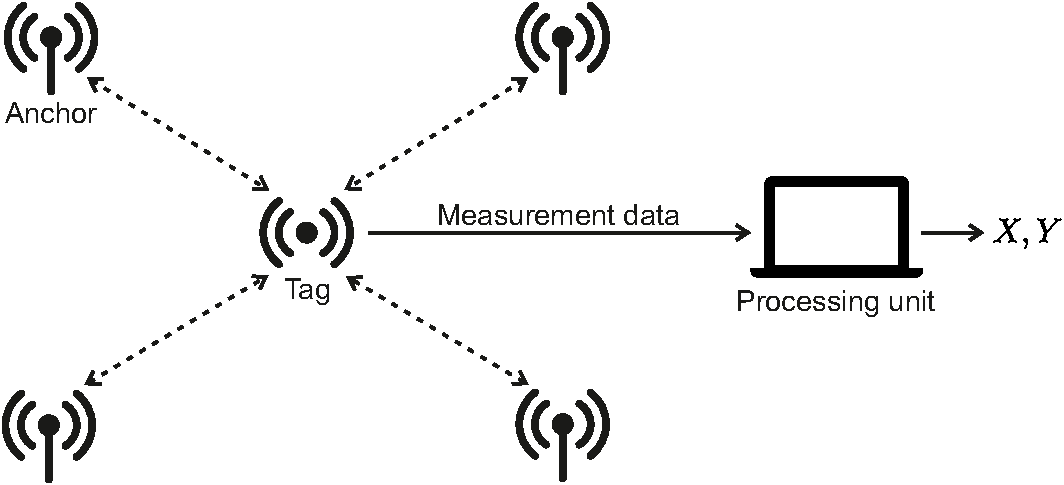
\includegraphics[width=0.75\textwidth]{Graphics/ips_topology.pdf}
\centering
\caption{Illustration of typical IPS topology.}
\label{fig:typical_topology}
\end{figure}

A typical IPS topology, illustrated in \autoref{fig:typical_topology}, often includes multiple wireless transceiver devices that communicate with one another to perform various measurements. These devices are commonly referred to as anchors and tags. Anchors are fixed devices with known, predefined locations, while tags are mobile devices (targets) whose positions are to be estimated. IPS setups usually include a central processing unit or localization engine that gathers measurement data and applies localization algorithms to infer the position of the tag.

\subsection{Measuring methods}
Wireless technologies can employ a number of measurement methods to infer the distance or direction to the anchor devices. These measurements, or their combinations, can be later used to infer the position of the tag. The principal methods are~\cite{mazhar2017precise}:

\begin{enumerate}
    \item \textbf{Phase of Arrival (PoA)}: Phase-based methods rely on the dependence between phase shift of the received signal and the distance it traveled in order to determine the range between transceivers:
    \begin{equation}
        \phi(f, x) = \frac{2\pi}{c}fx\,(\bmod\,2\pi),
    \end{equation}
    where $x$ is the distance, $f$ is the signal carrier frequency, and $c$ is the speed of light. For a known carrier frequency $f$ of the signal, the distance $x$ can be trivially inferred from the signal's phase shift $\phi$. To mitigate the effect of phase-wrapping, the received signal phase can be evaluated on multiple carrier frequencies, decreasing the ranging ambiguity. 
    
    \item \textbf{Angle of Arrival (AoA)}: AoA represents the direction from which a signal arrives at the receiver, and relies on measuring the phase or time difference of a signal arriving at multiple elements of an antenna array. The difference in arrival time $\Delta t$ and corresponding phase difference $\Delta \phi$ between two adjacent antennas, caused by a signal incident at an angle $\theta$, are given by:
    
    \begin{equation} 
    \Delta t = \frac{d \sin \theta}{c}, \qquad \Delta \phi = \frac{2\pi d \sin \theta}{\lambda}, 
    \end{equation}
    
    where $d$ is the antenna spacing, $c$ is the speed of light, and $\lambda$ is the signal wavelength. For known system parameters, these expressions allow the incident angle $\theta$ to be inferred from either time or phase measurements.
    
    \item \textbf{Received Signal Strength (RSS)}: RSS-bsed methods determine distance by analyzing the attenuation of the transmitted signal as it propagates through space. RSS relies on the path loss model, which describes how the power of a  signal decreases with distance. The power $P_r$ at a receiver located at a distance $d$ from a transmitter is given by:
    
    \begin{equation}
    P_r(d) = P_t - PL(d),
    \end{equation}
    where: $P_r(d)$ is the received power at distance $d$ (in dBm), $P_t$ is the transmitted power (in dBm), and $PL(d)$ is the path loss model (in dB). The path loss is often expressed as:
    \begin{equation}
    PL(d) = PL(d_0) + 10 \gamma \log_{10} \left( \frac{d}{d_0} \right) + X_{\sigma},
    \end{equation}
    where: $PL(d_0)$ is the reference path loss at a known reference distance $d_0$ (typically 1 meter), $\gamma$ is the path loss exponent, which depends on the environment, and $X_{\sigma}$ is a zero-mean Gaussian random variable representing shadowing effects.
    
    \item \textbf{Time-of-Arrival (ToA)}: ToA is a fundamental concept used in UWB systems to determine the Time-of-Flight of a signal. ToF is directly proportional to the distance between the transmitter and receiver:
    
    \begin{equation}
    d = c \cdot T_{\text{ToF}},
    \end{equation}
    where: $c$ is the speed of light, and $T_{\text{ToF}}$ is the measured time of flight.
    
    Sometimes this method is also referred to as Round-Trip-Time (RTT), which is double of ToF.
\end{enumerate}

\subsection{Positioning methods}
Once the distance or angle estimates are obtained using the methods described above, they can be used to compute the position of a target device using various localization techniques. These techniques include, but are not limited to: lateration, angulation, fingerprinting, and estimation filtering methods~\cite{qi2024current}.

\paragraph{Lateration and angulation nethods}
Lateration is used to determine the position of an unknown target based on distance measurements from multiple reference points (anchors). Angulation methods determine the position of the target using measured angles from at least two reference points.
The primary methods include trilateration, triangulation, and Time Difference of Arrival (TDoA).

\begin{enumerate}
    \item \textbf{Trilateration}
    Trilateration is a technique where the position of a target is estimated based on its measured distances from at least three known anchors in a 2D plane (or four anchors in 3D space). For each anchor $i$, the relationship between the known anchor position $(x_i, y_i)$ and the unknown target position $(x, y)$ is given by:
    
    \begin{equation}
    d_i = \sqrt{(x - x_i)^2 + (y - y_i)^2}
    \end{equation}
    
    where $d_i$ is the measured distance from the target to anchor $i$, and $(x_i, y_i)$ is the known position of the anchor. This results in a system of nonlinear equations, which can be solved using numerical methods such as least squares minimization.

    \item \textbf{Triangulation}
    Using known anchor positions and measured AoAs, the target position is obtained by solving the intersection of bearing lines. For two anchors at $(x_1, y_1)$ and $(x_2, y_2)$, the target’s coordinates are determined using:
    
    \begin{align}
    x &= x_i + d_i \cos \theta_i, \\
    y &= y_i + d_i \sin \theta_i,
    \end{align}
    
    where $\theta_i$ is the measured AoA at anchor $i$. With multiple AoA measurements, least squares estimation is typically used to obtain a position estimate.

    \item \textbf{Time Difference of Arrival (TDoA)}
    TDoA is a multilateration technique that relies on measuring the difference in signal arrival times at multiple spatially separated anchor nodes, rather than absolute arrival times. For two anchors located at $(x_1, y_1)$ and $(x_2, y_2)$, the corresponding range difference is given by:

    \begin{equation} 
    d_1 - d_2 = c \cdot (T_{\text{ToA}1} - T_{\text{ToA}_2}), 
    \end{equation}
    
    where $T_{\text{ToA}1}$ and $T{\text{ToA}_2}$ are the times of arrival of the signal at the two anchors, and $c$ denotes the speed of light. Each such measurement defines a hyperbolic constraint on the target's position. By combining measurements from at least three anchors, the position of the transmitting tag can be estimated by solving the resulting system of nonlinear equations. This method is widely used in UWB-based systems due to their high temporal resolution, which enables accurate time-based measurements.
\end{enumerate}

\paragraph{Fingerprinting}
The majority of fingerprinting methods are RSS-based~\cite{alarifi2016ultra}. However, to overcome the non-deterministic nature of signal attenuation, these methods establish a mapping between RSS and target position, rather than relying on analytical distance estimation. RSS fingerprinting typically consists of two phases:
\begin{enumerate}
    \item Offline Phase: A database of RSS measurements at known locations is created.
    \item Online Phase: The real-time RSS measurements are compared with the fingerprint database to estimate the most probable location.
\end{enumerate}
A common approach for position estimation is k-Nearest Neighbors (k-NN), where the estimated position is given by:

\begin{equation}
(x, y) = \frac{1}{k} \sum_{i=1}^{k} (x_i, y_i),
\end{equation}

where $(x_i, y_i)$ are the positions of the $k$ closest fingerprint database entries.

\subsection{Filtering methods}\label{kalman_theory}
In wireless systems, the measurement noise and multipath interference are unavoidable effects that can degrade localization accuracy. To address this, various filtering techniques are employed to improve the robustness of position estimates and enable sensor fusion, as discussed in \autoref{related_work}. Among the wide range of approaches, including particle filters for non-Gaussian systems~\cite{wang2014particle}, Kalman filters (KF) and their variants remain the most widely used due to their balance of computational efficiency and estimation accuracy.

Kalman filters recursively estimate the state of a system by using prior knowledge to infer the current state of the target in a way that minimizes the error between the prediction and the actual state. Originally, KF was designed to work with linear-space states, considering that the measurement noise obeys a Gaussian distribution. However, there are versions of KF adapted to estimate states in nonlinear systems such as Extended Kalman filter (EKF) or Unscented Kalman filter (UKF)~\cite{wan2000unscented, konatowski2016comparison}.

\paragraph{Standard Kalman Filter}

The Kalman Filter is based on a discrete-time linear dynamic system~\cite{wiley_kalman}:
\begin{align}
    \mathbf{x}_k &= \mathbf{F}_{k} \mathbf{x}_{k-1} + \mathbf{w}_{k}, \quad \mathbf{w}_{k-1} \sim \mathcal{N}(0, \mathbf{Q}_{k-1}) \\
    \mathbf{z}_k &= \mathbf{H}_k \mathbf{x}_k + \mathbf{v}_k, \quad \mathbf{v}_k \sim \mathcal{N}(0, \mathbf{R}_k)
\end{align}
where $\mathbf{x}_k$ is the system state vector, $\mathbf{z}_k$ is the measurement vector,  and $\mathbf{F}_k$, and $\mathbf{H}_k$ are the state transition and observation matrices, respectively. $\mathbf{w}_{k-1}$ and $\mathbf{v}_k$ are the process and measurement noise, modeled as zero-mean Gaussians with covariances $\mathbf{Q}_{k-1}$ and $\mathbf{R}_k$.

At each time step, KF performs the following predict and update steps:

\emph{Prediction:}
\begin{align}
    \hat{\mathbf{x}}_k^- &= \mathbf{F}_k \hat{\mathbf{x}}_{k-1} \\
    \mathbf{P}_k^- &= \mathbf{F}_k \mathbf{P}_{k-1} \mathbf{F}_k^\top + \mathbf{Q}_{k-1}
\end{align}

\emph{Update:}
\begin{align}
    \mathbf{K}_k &= \mathbf{P}_k^- \mathbf{H}_k^\top \left( \mathbf{H}_k \mathbf{P}_k^- \mathbf{H}_k^\top + \mathbf{R}_k \right)^{-1} \\
    \hat{\mathbf{x}}_k &= \hat{\mathbf{x}}_k^- + \mathbf{K}_k (\mathbf{z}_k - \mathbf{H}_k \hat{\mathbf{x}}_k^-) \\
    \mathbf{P}_k &= (\mathbf{I} - \mathbf{K}_k \mathbf{H}_k) \mathbf{P}_k^-,
\end{align}

where $\mathbf{K}_k$ is the Kalman gain, $\hat{\mathbf{x}}_k$ is the posterior state estimate, and $\mathbf{P}_k$ is the corresponding covariance.

\paragraph{Extended Kalman Filter}
When the system dynamics are nonlinear, the Kalman Filter is extended by linearizing the system using a first-order Taylor series expansion. The nonlinear system is given by~\cite{wiley_kalman}:
\begin{align}
    \mathbf{x}_k &= \bm{f}(\mathbf{x}_{k-1}) + \mathbf{w}_{k-1} \\
    \mathbf{z}_k &= \bm{h}(\mathbf{x}_k) + \mathbf{v}_k
\end{align}
where $\bm{f}$ and $\bm{h}$ are nonlinear state transition and observation functions. In EKF, the state and observation matrices are approximated by their Jacobians:
\begin{align}
    \mathbf{F}_{k} &= \left.\frac{\partial \bm{f}}{\partial \mathbf{x}}\right|_{\hat{\mathbf{x}}_{k-1}} , \quad
    \mathbf{H}_k = \left.\frac{\partial \bm{h}}{\partial \mathbf{x}}\right|_{\hat{\mathbf{x}}_k^-}
\end{align}

EKF then performs the similar prediction and update steps as in the standard KF. The EKF is considered the de-facto standard approach for approximation of nonlinear systems' state~\cite{julier2004unscented}.

% \paragraph{Unscented Kalman Filter (UKF)}
% The Unscented Kalman Filter (UKF) addresses the limitations of the EKF in handling highly nonlinear systems by avoiding direct linearization of nonlinear functions $\bm{f}$ and $\bm{h}$. Instead of computing Jacobians as in EKF, UKF uses a deterministic sampling approach known as the unscented transform to propagate a minimal set of carefully chosen sample points, called sigma points, through the nonlinear functions to obtain the estimate of the system state~\cite{wan2000unscented}.

% Initially, a set of sigma points is generated from the prior state estimate \(\hat{\mathbf{x}}_{k-1}\) and its associated covariance \(\mathbf{P}_{k-1}\):
% \begin{align}
%     \mathcal{X}_{k-1} &= \left[\hat{\mathbf{x}}_{k-1}, \quad \hat{\mathbf{x}}_{k-1} \pm \sqrt{(n+\lambda)\mathbf{P}_{k-1}}\right]
% \end{align}
% where $n$ is the dimension of the state vector, and $\lambda$ is a first-order scaling parameter that controls the distribution of sigma points around the mean. Each sigma point is propagated through the nonlinear state transition and observation functions:
% \begin{align}
%     \mathcal{X}_k &= f(\mathcal{X}_{k-1}, \mathbf{u}_{k-1}) \\
%     \mathcal{Z}_k &= h(\mathcal{X}_k)
% \end{align}

% The predicted state mean and covariance, as well as measurement predictions, are computed using weighted averages of the transformed sigma points.

% Compared to EKF, UKF provides more accurate estimates of the true mean and covariance in strongly nonlinear environments by preserving higher-order terms during the propagation, albeit at a higher computational cost~\cite{konatowski2016comparison}.

% \subsubsection{Particle Filters}
% The particle filtering algorithm was proposed for dealing with non-linear and non-Gaussian systems, commonly seen in real-world setups. It works by representing the posterior distribution of the system's state using a set of weighted particles that are propagated and re-sampled over time~\cite{wang2014particle}:

% \begin{equation}
% p(\mathbf{x}_k | \mathbf{z}_{1:k}) \approx \sum_{i=1}^{N} w_k^i \delta(\mathbf{x}_k - \mathbf{x}_k^i),
% \end{equation}

% where: $\mathbf{x}_k^i$ are particle samples, $w_k^i$ are their respective weights. Particle filters often outperform Kalman filters in non-Gaussian environments, making them suitable for complex indoor localization~\cite{elsanhoury2022precision}.

\section{Wireless technologies}

\subsection{Overview}
\paragraph{Wi-Fi}
Wi-Fi, an IEEE 802.11 standard~\cite{ieee80211}, is a wireless technology widely used for Wireless Local Area Networks (WLANs), operating on 2.4, 5, or 6 \si{\giga\hertz} bands with typical channel widths of 20 \si{\mega\hertz}.

The majority Wi-Fi-based positioning methods rely on RSS fingerprinting~\cite{leitch2023indoor}. However, RSS is inherently unreliable due to variability from obstacles and reflections, making it difficult to establish a consistent relationship between RSS and distance~\cite{Asaad2022Review}. Therefore, to improve accuracy, standardization bodies have introduced alternative methods. For example, in 2016, the IEEE 802.11mc amendment added Fine-Time Measurements (FTM) to Wi-FI, enabling distance estimation via round-trip time (RTT) with sub-meter accuracy.

\paragraph{BLE}
Bluetooth Low-Energy (BLE), developed by the Bluetooth Special Interest Group (SIG), is a wireless technology for Personal Area Networks (PANs), operating in the \SI{2.4}{\giga\hertz} band with 1–2 \si{\mega\hertz} wide channels.

Similarly to Wi-Fi, BLE typically uses RSS-based localization~\cite{leitch2023indoor}. However, in 2019, Bluetooth 5.1 specification introduced Direction Finding feature, which provides In-Phase and Quadrature (IQ) samples of the received signal, enabling for phase-based measurements. Bluetooth 6.0 later introduced Channel Sounding, combining phase and RTT measurements for sub-meter accuracy ranging estimates.

% \subsubsection{Wi-Fi}
% Wi-Fi (IEEE 802.11 standard~\cite{ieee80211}) is a wireless technology widely known for usage within Wireless Local Area Networks (WLANs). Common WiFi networks operate on 2.4 GHz, 5 GHz, or 6 GHz bands, typically utilizing 20 MHz channel width.

% The majority of Wi-Fi-based approaches make use of RSS fingerprinting for position estimation~\cite{leitch2023indoor}. However, RSS-based localization is inherently unreliable because signal strength is influenced by obstacles and reflections, making it difficult to establish a consistent relationship between RSS and distance~\cite{Asaad2022Review}. Therefore, standardization bodies have been working on alternatives to improve localization accuracy. In 2016, WiFi introduced Fine-Time Measurements (FTM) in the IEEE 802.11mc standard, enabling distance estimation using round-trip time (RTT) with sub-meter accuracy. 

% \subsubsection{Bluetooth Low-Energy (BLE)}
% Bluetooth LE is a wireless technology developed by Bluetooth Special Interest Group (Bluetooth SIG) used in Personal Area Networks (PAN). Bluetooth operates in 2.4 GHz band, divided into 1/2 MHz wide channels. 

% Similar to Wi-Fi, BLE often relies on some form of RSS-based localization methods~\cite{leitch2023indoor}. In 2019, Bluetooth 5.1 Core Specification introduced a Direction Finding feature that provided In-Phase and Quadrature (IQ) samples of the received signal, enabling for phase-based measurements. Later, Bluetooth 6.0 introduced Channel Sounding, that combines phase-based and round-trip time measurements to provide sub-meter ranging estimates.

\paragraph{UWB}
Ultra-wide Band (UWB) is an IEEE 802.15.4a/z standard~\cite{ieee802154}  impulse radio technology, commonly used specifically for indoor positioning tasks. Unlike other, narrow-band technologies, such as Wi-Fi or Bluetooth, UWB uses wide band width, typically around 500-1000 \si{\mega\hertz}, operating on 3.1-10.6 \si{\giga\hertz} frequencies.

For distance estimation, UWB systems rely on precise Time-of-Flight measurements. The key advantage of UWB systems is high resolution, made possible by transmitting short pulses in time-domain. This allows UWB to distinguish between multipath components and makes it immune to interference effects, allowing a centimeter-level accuracy. In addition, relatively low center frequency still allows UWB signals to penetrate the obstacles~\cite{cheraghinia2024comprehensive}.

\subsection{Technical details}

The underlying drawbacks of using narrow-band technologies in positioning systems lie in their low-level specifics. These include modulation schemes and signal bandwidth. A modulation is the process of encoding digital information into signals by modifying some of their physical characteristics. The bandwidth refers to the range of frequencies contained within a generated signal.

\subsubsection{Modulation schemes}

% \begin{figure}[h!]
% 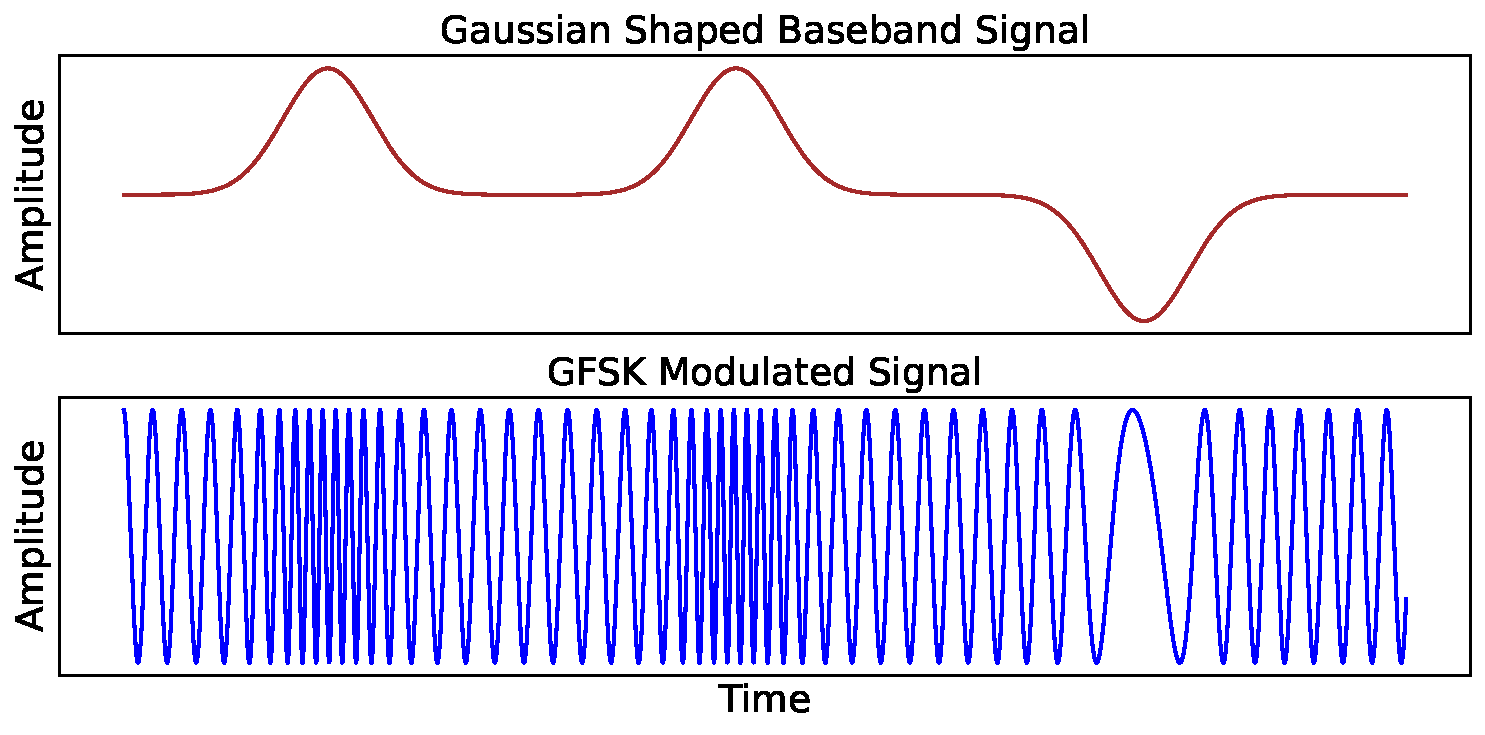
\includegraphics[width=0.7\textwidth]{Graphics/gfsk.pdf}
% \centering
% \caption{BLE signal modulation illustration (simplified)}
% \label{fig:ble-mod}
% \end{figure}

BLE uses a modification of Frequency-Shift Keying (FSK) -- Gaussian FSK (GFSK), where data is encoded as frequency deviations from a central continuous wave carrier:

\begin{equation}
S(t) = A e^{j\left(2\pi (f_c t + \Delta f \int_{0}^{t} m(\tau) d\tau)\right)},
\end{equation}

where: $A$ is the signal amplitude, $f_c$ is the carrier frequency, $\Delta f$ is the frequency deviation, $m(t)$ is the data-modulating function. 

% The illustration of GFSK-based scheme is provided in Fig.\autoref{fig:ble-mod}

Wi-Fi primarily employs Orthogonal Frequency-Division Multiplexing (OFDM), where data is transmitted over multiple orthogonal subcarriers. Each subcarrier is modulated using Binary Phase-Shift Keying (BPSK), Quadrature Phase-Shift Keying (QPSK), or higher-order modulations such as 16-QAM or 64-QAM. The baseband OFDM signal is expressed as:

\begin{equation}
S(t) = \sum_{k=0}^{N-1} X_k e^{j 2 \pi f_k t},
\end{equation}

where: $X_k$ is the symbol modulated onto the $k$-th subcarrier, $f_k$ is the subcarrier frequency,
$N$ is the number of subcarriers.

\begin{figure}[tbh]
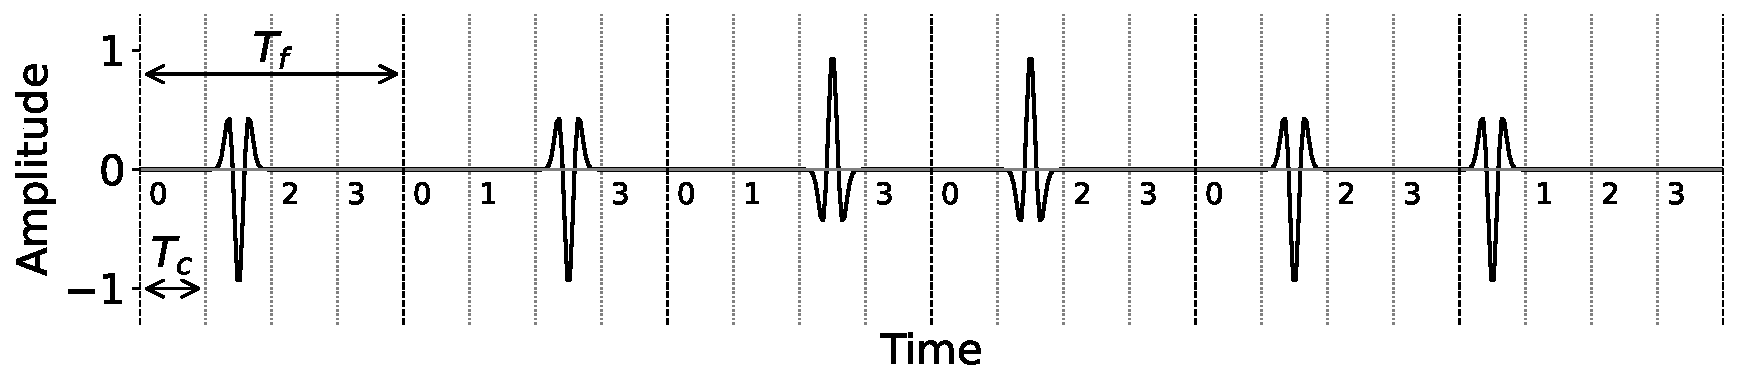
\includegraphics[width=0.85\textwidth]{Graphics/uwb_bpsk.pdf}
\centering
\caption{Conceptual illustration of a UWB signal BPM/BPSK modulation .}
\label{fig:uwb-mod}
\end{figure}

Unlike narrow-band technologies, UWB is an Impulse Radio (IR) technology. It transmits short sequences of narrow pulses with the duration in the sub-nanosecond order, and uses pulse-based modulation scheme, which is typically a ternary modulation, achieved through the combination of:

\begin{itemize}
    \item Binary Phase-Shift Keying (BPSK): The phase of each pulse is shifted by 180° to encode binary data. For BPSK, the transmitted signal is given by:
    \begin{equation}
    S(t) = A p(t) e^{j (\pi m_n)},
    \end{equation}
    where: $A$ is the amplitude of the transmitted pulse, $p(t)$ is the pulse shaping function, and $m_n \in \{0, 1\}$ is the modulating bit.

    \item Burst Position Modulation (BPM): The information is encoded by the position of the transmitted pulse in a time slot. For BPM, the transmitted signal can be expressed as:
    \begin{equation}
    S(t) = A p\left(t - m_n T_c\right), \quad T_c = T_f / M
    \end{equation}
    where: $T_c$ is the chip duration, $m_n \in \{0, 1, \dots, M-1\}$ selects one of $M$ available slots within a time frame $T_f$, and $p(t)$ is the pulse shape.
\end{itemize}

\autoref{fig:uwb-mod} illustrates a UWB signal with BPM/BPSK modulation. Each bit is represented by a sequence of two impulses, spaced by one frame duration $T_f$. The position of each pulse within its frame is defined by a time-hopping code  $m_n \in \{0, 1, 2, 3\}$, selecting one of $M = 4$ slots of duration $T_c$, while polarity is modulated using BPSK to encode the binary value. This example transmits the binary sequence:  
$$
\boxed{0\ 1\ 0}
$$ 
with time-hopping code:  
$$
\{1, 2\},\ \{2, 1\},\ \{1, 0\}.
$$ 

\subsubsection{Bandwidth}
The use of ultrashort pulses in ultra-wideband systems enables exceptionally high temporal resolution, which is critical for precise estimation of the signal's time of arrival and, consequently, accurate time-of-flight measurements. This capability is governed by the time–bandwidth uncertainty principle, which imposes a lower bound on the product of time duration $\Delta t$ and bandwidth $\Delta f$:

\begin{equation} \Delta t \cdot \Delta f \geq \frac{1}{2}. \end{equation}

The spatial resolution $\Delta D$ associated with ToF-based ranging is therefore given by:

\begin{equation} \Delta D = \frac{c}{2\Delta f}, \end{equation}

where $c$ is the speed of light in free space. Accordingly, larger bandwidths directly improve ranging precision.

In practical terms, achieving finer resolution in the time domain requires broader spectral occupancy in the frequency domain. This time-frequency duality is formally described by the Fourier Transform:

\begin{equation} 
\mathcal{F}{x(t)} = X(f) = \int_{-\infty}^{\infty} x(t) e^{-j2\pi ft} , dt, 
\end{equation}



which decomposes a time-domain signal $x(t)$ into its frequency-domain representation $X(f)$. A canonical example is the Dirac delta function $\delta(t)$, which satisfies:

\begin{equation} \mathcal{F}{\delta(t)} = 1, \end{equation}

indicating that a theoretically infinitesimal pulse contains all frequencies with equal amplitude -- i.e., infinite bandwidth. While physical systems cannot generate true delta functions, UWB pulses (e.g., Gaussian monocycles or higher-order derivatives) approximate this behavior, exhibiting wide spectral occupancy and short temporal duration.

% \begin{figure}[h!]
% 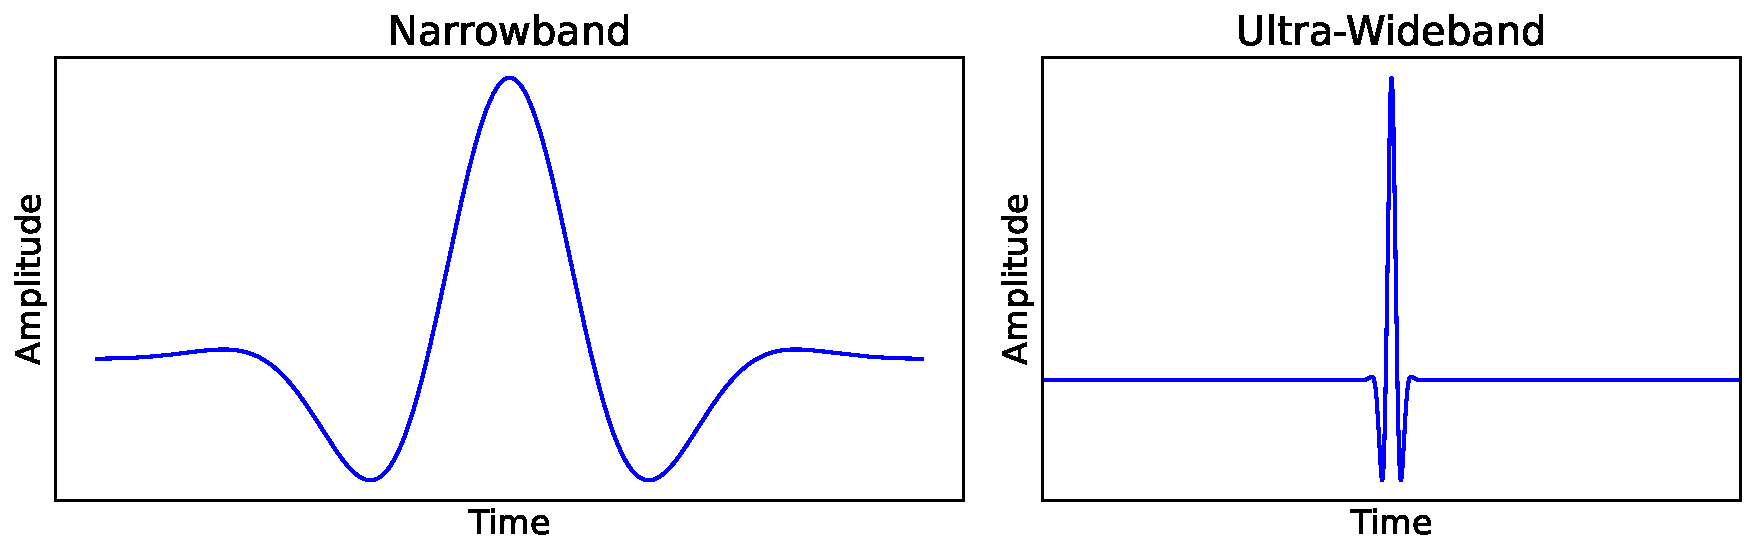
\includegraphics[width=0.75\textwidth]{Graphics/narrowband_vs_uwb.pdf}
% \centering
% \caption{Comparison of a UWB impulse signal and a narrowband (BLE/Wi-Fi) waveform.}
% \label{fig:uwbvsnb}
% \end{figure}

UWB's bandwidth of \SI{500}{\mega\hertz} or more correlates with sub-nanosecond temporal resolution and centimeter-level ranging accuracy. In contrast, conventional narrowband systems (e.g., BLE, Wi-Fi) transmit signals with limited bandwidth (1–20 \si{\mega\hertz}), yielding time resolution of tens to hundreds of nanoseconds. This restricts their temporal and spatial resolution, leading to ranging errors in the order of meters. % The difference in time-domain characteristics is illustrated in Fig.\autoref{fig:uwbvsnb}. 
Additionally, the usage of continuous waves makes them susceptible to multipath interference. Together, this renders narrowband technologies unsuitable for fine-grained localization in multipath-dense environments.

However, to precisely estimate the ToF, UWB still has to to distinguish the actual direct signal path from multipath components. For this purpose, UWB relies on Leading Edge Detection (LDE) algorithms. LDE operate on Channel Impulse Response (CIR) (refer to \autoref{principles}).

\section{UWB principles}\label{principles}
\subsection{UWB frame}

\begin{figure}[tbh]
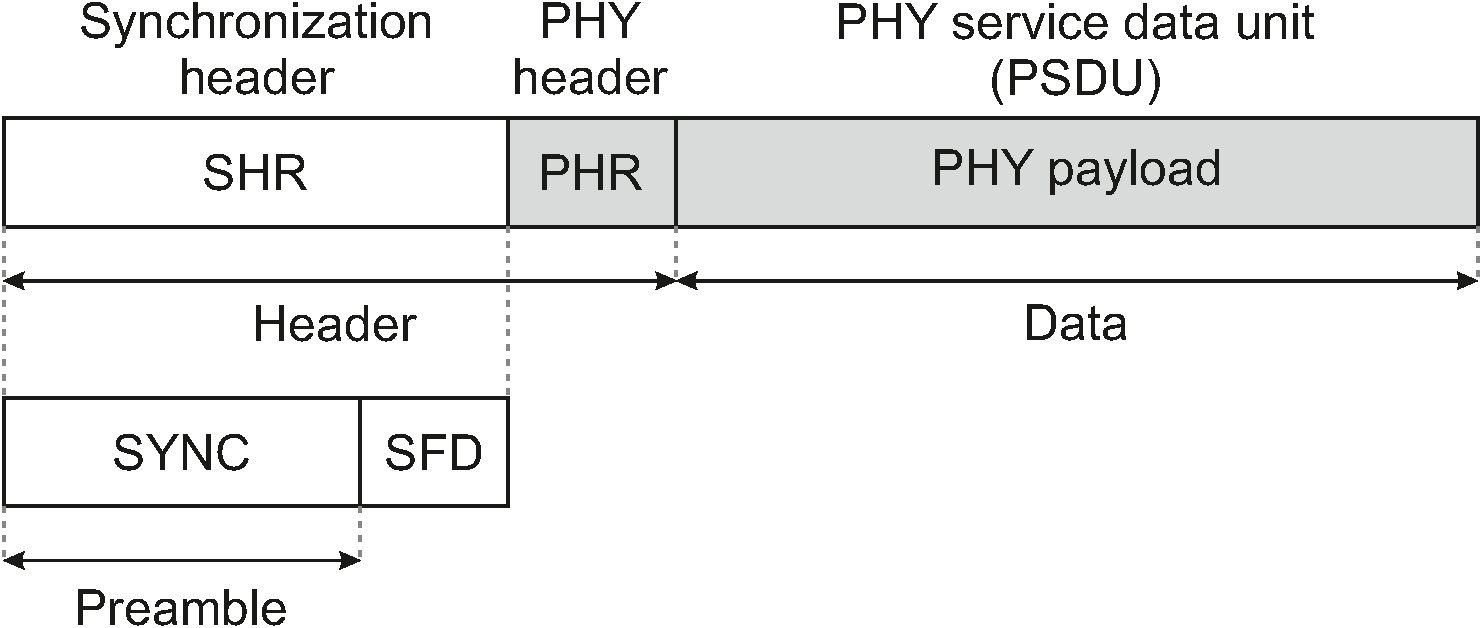
\includegraphics[width=0.6\textwidth]{Graphics/uwb_phy.pdf}
\centering
\caption{IEEE 802.15.4a UWB physical layer frame structure.}
\label{fig:phy}
\end{figure}

IEEE 802.15.4a standard-compliant UWB packet format (see \autoref{fig:phy}) follows the below structure:
\begin{itemize}
    \item Synchronization Header (SHR): Contains the preamble (SYNC) and SFD (start of frame
delimiter) sequences, used for timing acquisition and synchronization.
    \item Physical Header (PHR): Encodes frame control information.
    \item Data Payload: Contains the transmitted information.
\end{itemize}


% \begin{figure}[h!]
% \includegraphics[width=8cm]{Graphics/preamble.png}
% \centering
% \caption{Example of the modulated preamble code.}
% \label{fig:preamble}
% \end{figure}
%TODO!: Review whether this is really needed here...

The synchronization header of the frame is particularly relevant for UWB ranging capabilities, as it contains the preamble used for CIR reconstruction. In SHR, a SYNC sequence, or preamble, is transmitted first. It consists of the repetition of known sequence codes. %Fig.\autoref{fig:preamble} shows the example of the modulated preamble code. 
The codes used in the preamble are defined in the standard, and are part of family of codes known as perfect ternary sequences~\cite{mcelroy2014comparison}. These codes are constructed using a ternary alphabet $\{0, -1, 1\}$ to possess unique perfect periodic autocorrelation properties. 

The autocorrelation function of a sequence $\bm s$ of length $N$ for shift $\tau$ is given by:
\begin{equation}
R(\tau) = \sum_{i=0}^{N-1} \bm s_i \cdot \bm s_{i+\tau \bmod N}.
\end{equation}
A sequence has perfect periodic autocorrelation if all off-peak ($\tau \ne 0 \bmod N$) autocorrelation values are zero~\cite{blake2014construction}:

\begin{equation}
R(\tau) =
\begin{cases}
    N, & \tau = 0 \bmod N,\\
    0, & \tau \neq 0 \bmod N.
\end{cases}
\end{equation}

The perfect autocorrelation property ensures that once the presence of a transmission is detected by the receiver device, the remainder of the preamble can be used for CIR estimation~\cite{mcelroy2014comparison}.

\subsection{Channel impulse response}\label{cir_theory}

\begin{figure}[tbh]
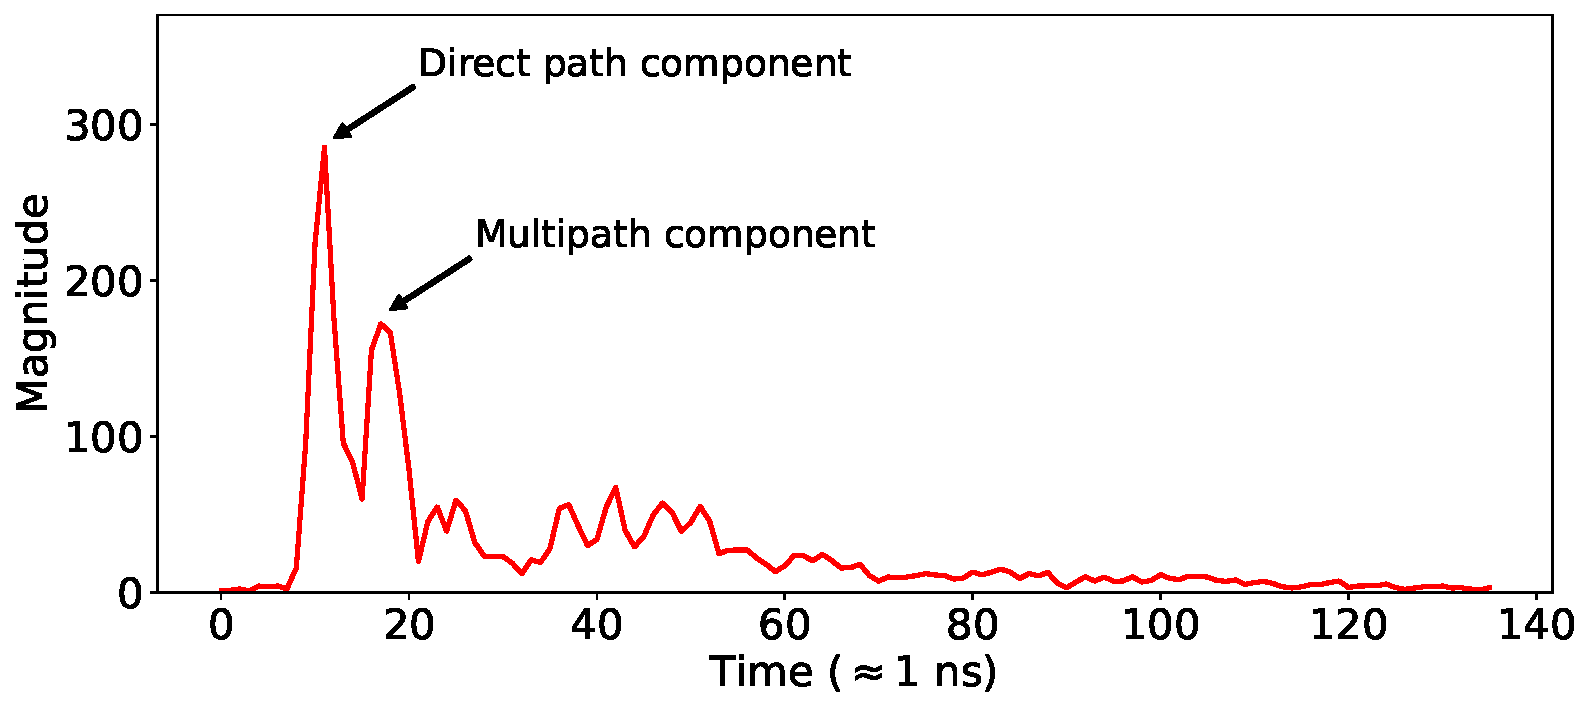
\includegraphics[width=0.75\textwidth]{Graphics/saved_sample.pdf}
\centering
\caption{Example of UWB Channel Impulse Response.}
\label{fig:cir}
\end{figure}

Channel Impulse Response (CIR) is fundamental characteristic of any UWB system. The receiving device estimates CIR by correlating a known preamble sequence with a received signal. CIR $h(t)$ is often modeled as~\cite{cheraghinia2024comprehensive}:

\begin{equation}
h(t) = \sum_{i} a_i \delta(t - \tau_i) + \nu(t),
\end{equation}

where $a_i$ and $\tau_i$ represent the amplitude and delay of the $i$-th multipath component, respectively, $\delta(t)$ denotes the Dirac delta function, and $\nu(t)$ represents diffuse multipath components. The first term encapsulates multipath propagation phenomena, where the transmitted signal is propagated to the receiver through multiple paths, arriving with different delays. The second term models random noise, typically with Additive white Gaussian noise (AWGN).

To this end, CIR characterizes how an impulse signal propagates through the wireless channel and captures the features of the propagation environment. Typical accumulator of Channel Impulse Response is presented in the \autoref{fig:cir}. The sampling interval of the CIR is equal to half of the period of the fundamental frequency (FF), which is typically around \SI{1}{\nano\second} for \SI{500}{\mega\hertz} FF. Consequently, each sample of the CIR corresponds to a distance of \SI{\approx 30}{\centi\metre} (given that UWB signal propagates through the air medium). As was noted before, such high temporal resolution allows UWB to distinguish between multiple paths, achieving precise ToF estimation. This process is performed by LDE algorithm.

\subsubsection{Leading edge detection}\label{lde}

\begin{figure}[tbh]
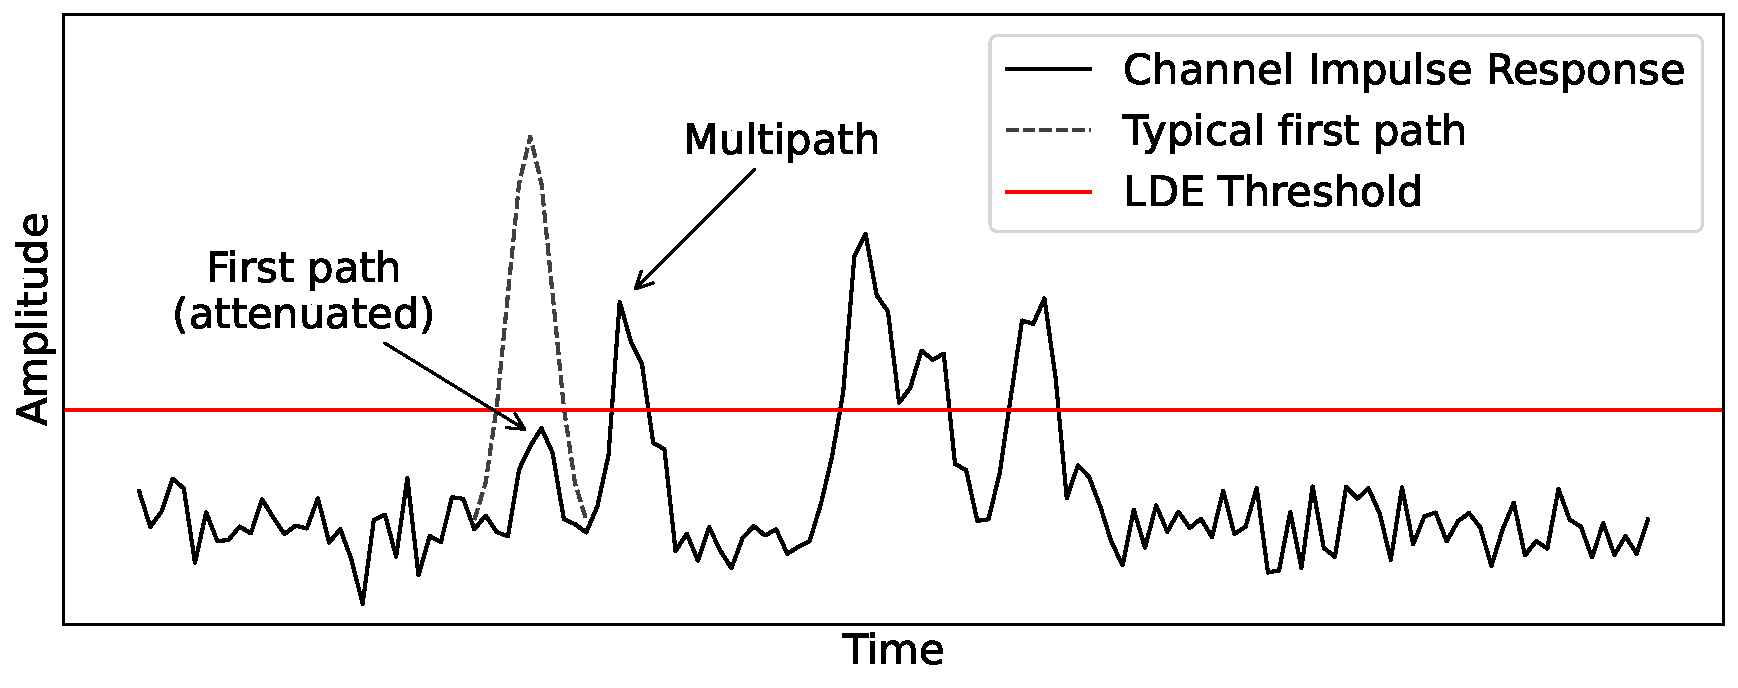
\includegraphics[width=0.8\textwidth]{Graphics/uwb_lde_error.pdf}
\centering
\caption{Conceptual illustration of undetected first path in LDE process.}
\label{fig:lde-nlos}
\end{figure}

The Leading Edge Detection (LDE) algorithm operates on CIR, aimed at identifying the actual first arriving path (FP), ensuring accurate time-stamping. The goal of LDE is to select the detection threshold in a most reliable way, so to locate the first significant peak in the CIR, while preventing the confusion of the FP with multipath components or channel noise:

\begin{equation}
\tau_{\text{LE}} = \arg \min_{\tau} \{ h(\tau) \geq \theta_{\text{LDE}} \},
\end{equation}

where $\theta_{\text{LDE}}$ is a detection threshold, and and $\tau_{\text{LE}}$ is the estimated arrival time of the first path.


Given LoS propagation, the LDE algorithm can produce accurate time-stamps. However, in severe NLoS cases, the direct path signal can be attenuated to the extent that no longer allows the LDE to work reliably, and the reported time-stamp will correspond to the reflected signal. Such scenario is presented in \autoref{fig:lde-nlos}.

\subsection{Ranging techniques}
\subsubsection{Two-Way ranging}\label{theory:twr}

\begin{figure}[tbh]
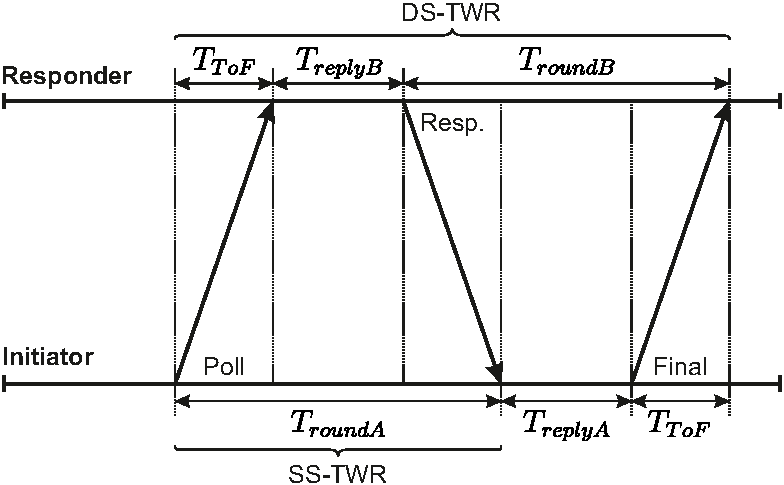
\includegraphics[width=0.7\textwidth]{Graphics/twr.pdf}
\centering
\caption[Two-way ranging exchange.]{Two-way ranging exchange (single-sided and double-sided).}
\label{fig:twr}
\end{figure}

ToF estimation with single, one-way communication, requires precise clock sycnhronization between tag and anchor devices. This is extremely hard to achieve, as centimeter-level precision in ToF estimation requires clock difference to be in the order of picoseconds. Therefore, UWB systems often rely on Two-Way Ranging (TWR) to accurately determine distance, eliminating the need for precise time synchronization between devices. TWR works by measuring the round-trip time of signals.

\paragraph{SS-TWR}
The simplest form of TWR is Single-Sided Two-Way Ranging (SS-TWR), where a responder device (B) sends a reply upon receiving a request signal from initiator device (A). \autoref{fig:twr} illustrates the ranging exchange in the TWR process. The ToF is then inferred from the following equation:

\begin{equation}\label{tof-ss}
T_{ToF} = \frac{1}{2} (T_{roundA} - T_{replyB}),
\end{equation}

where $T_{replyB}$ is the time delay at the responder, and $T_{ToF}$ is the time-of-flight. Under ideal conditions, $T_{ToF}$ can be precisely estimated. However, this estimate can still be largely affected by the clock drift~\cite{neirynck2016alternative}.

\paragraph{DS-TWR} 
To mitigate clock drift errors, Double-Sided Two-Way Ranging (DS-TWR) is used. DS-TWR adds a symmetrical exchange to SS-TWR by sending additional message from the initiator back to the responder upon the reception of the reply message. Similarly to SS-TWR (\autoref{tof-ss}), in DS-TWR the ToF is derived from the following system of equations: 

\begin{equation}
\begin{cases}
T_{roundA} = T_{replyB} + 2T_{ToF}\\
T_{roundB} = T_{replyA} + 2T_{ToF}
\end{cases}
\end{equation}

\begin{equation}
T_{ToF} = \frac{1}{4} (T_{roundA} - T_{replyB} + T_{roundB} - T_{replyA}).
\end{equation}

However, this approach has a limitation due to assumption that the reply delays $T_{replyX}$ will be equal on both sides~\cite{neirynck2016alternative}. 

\paragraph{ADS-TWR}\label{adstwr}
A variation known as Alternative DS-TWR (ADS-TWR) has been proposed by Neirynck et al. in 2016~\cite{neirynck2016alternative}. ADS-TWR eliminates the requirement for equal reply delays, reducing complexity of the system and improving ToF estimation accuracy. Instead of relying on reply delay symmetry, it applies:

\begin{equation}
T_{ToF} = \frac{T_{roundA}T_{roundB} - T_{replyA}T_{replyB}}{T_{roundA} + T_{replyA} + T_{roundB} + T_{replyB}}.
\end{equation}

This method minimizes the impact of the clock drift error, making it more robust for practical implementations.

\subsubsection{Time-division multiple access}\label{tdma}

% \begin{figure}[h!]
% \includegraphics[width=8cm]{Graphics/tdma.png}
% \centering
% \caption{TDMA timing diagram}
% \label{fig:tdma}
% \end{figure}
% TODO: Do we really need this?

Generally, it is desirable to obtain the measurement result on the tag device to minimize system complexity. However, due to the nature of DS-TWR, this requires the measurement to be initiated by the anchor, as it would otherwise be necessary to introduce additional exchanges that would degrade the system's performance in terms of ranging frequency. Consequently, this poses a problem of synchronization between multiple anchor devices to prevent them from ranging simultaneously and avoid cross-interference. 

To solve this problem, Time-Division Multiple Access (TDMA) method is used. TDMA is a channel access method, that allows multiple devices to share the same channel by dividing the ranging process into different time slots, preventing signal collisions~\cite{falconer1995time}. The process is as follows:

\begin{itemize}
    \item The network controller (tag) assigns a time slot to each ranging device (anchor).
    \item Devices transmit signals only within their allocated slots.
    \item Receivers process only signals within the designated time windows, preventing overlap.
\end{itemize}

Originally, TDMA was used in the satellite communication systems, but later was also adopted in UWB TWR-based systems. 

% Schematic timing diagram illustrating the TDMA-based approach can be found in Fig.\autoref{fig:tdma}. 

\section{Sources of errors}\label{error_sources}

\begin{figure}[tbh]
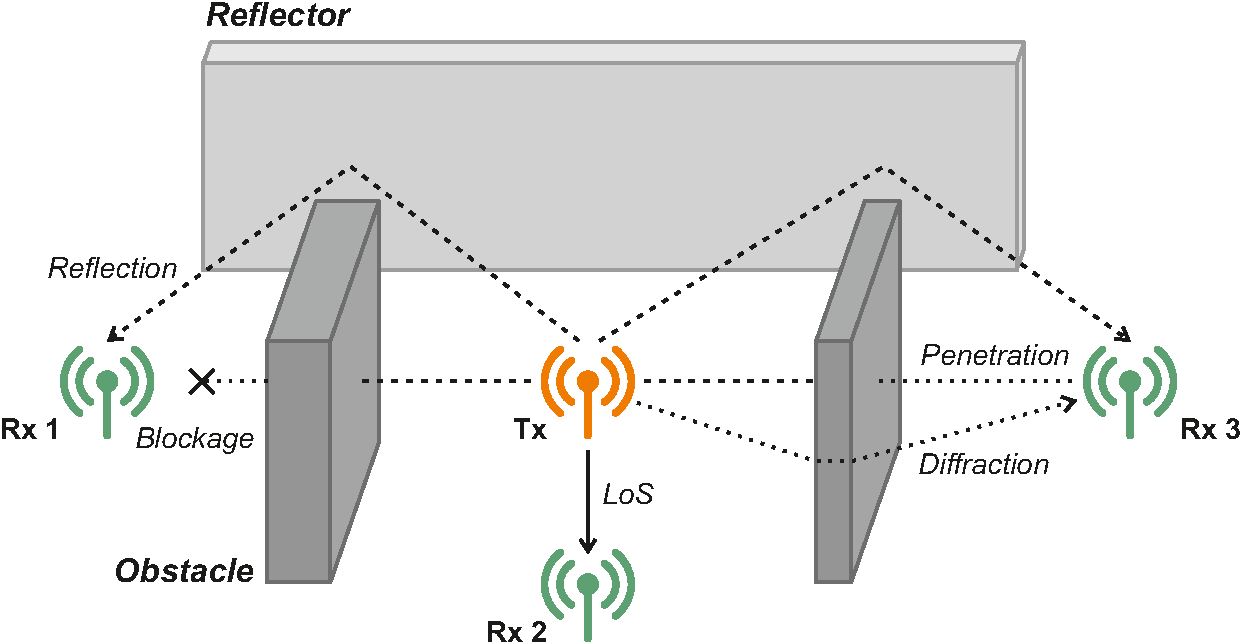
\includegraphics[width=0.75\textwidth]{Graphics/obstacles.pdf}
\centering
\caption[Illustration of error sources in UWB systems.]{Illustration of error sources in UWB systems. The transmitter (Tx) communicates with three receivers (Rx 1-3) under different conditions: complete signal blockage (Rx 1), LoS propagation (Rx 2), and multipath propagation (Rx 3) involving reflection, diffraction, and obstacle penetration.}
\label{fig:error_nlos}
\end{figure}

Despite the high precision of UWB-based ranging systems, several error sources affect their performance, particularly in indoor and multipath-rich environments. These include Non-Line-of-Sight (NLOS) propagation, multipath interference, and refraction effects~\cite{dardari2009ranging}. The schematic in \autoref{fig:error_nlos} illustrates the principal NLoS conditions.

\paragraph{Multipath interference}

Multipath occurs when multiple copies of the transmitted signal arrive at the receiver via different paths due to reflections, diffractions, and scattering. UWB systems are generally resilient to multipath because of their short pulses, which allow separation of distinct paths in the Channel Impulse Response (CIR). This phenomena is discussed in \autoref{cir_theory}. However, in dense multipath environments, the LDE algorithm can misclassify later multipath component as the actual direct path, introducing a positive bias in the estimated range:

\begin{equation}\label{multipath_err}
    \Delta d =  \tau_i c,
\end{equation}

where $\tau_i$ is the delay of the $i$-th multipath component.

\paragraph{NLoS propagation}

NLOS propagation occurs when the direct path between the transmitter and receiver is obstructed, and the first arriving signal is a reflected, refracted, or diffracted version of the original pulse. This also introduces a positive bias in the estimated range. In case of partial NLoS, where the direct path still exists but passes through a refractive material (e.g., a wall or furniture), which slows the signal down, the measurement error is modeled as:

\begin{equation}
\Delta d = (\sqrt{\epsilon_r} - 1) d_o,
\end{equation}
where $d_o$ is the thickness of the obstacle, and $\epsilon_r$ is its relative permittivity. 

In the case of complete blockage, the receiver can only observe the reflected or diffracted multipath signal components, therefore reporting wrong distance estimate. This effect is illustrated in \autoref{lde}. The error model is analogous to the multipath case (\autoref{multipath_err}) described above. Empirically, the resulting range bias $b_r$ is often modeled as a log-normal random variable:

\begin{equation}
b_r \sim \text{Lognormal}(\mu, \sigma^2).
\end{equation}

This effect of error can be reduced by NLoS identification and mitigation techniques, such as machine learning models, discussed in \autoref{related_work}.

\paragraph{Geometric dilution of precision}

In addition to measurement errors, the accuracy of UWB positioning systems is fundamentally influenced by the geometric configuration of anchor nodes.

This impact is quantified by the Geometric Dilution of Precision (GDOP), a metric that describes how uncertainty in distance measurements propagates to uncertainty in estimated position. Consider $N$ anchor nodes located at known positions $\mathbf{p}_{A_i} = (x_{A_i}, y_{A_i})$ for $i = 1, \dots, N$, and a tag at position $\mathbf{p}_T = (x_T, y_T)$. The measured distance from the tag to the $i$-th anchor is given by:

\begin{equation}
d_i = \|\mathbf{p}_T - \mathbf{p}_{A_i}\|.
\end{equation}

Linearizing the system of distance equations around an estimate $\mathbf{p}_0 = (x_0, y_0)$ yields the Jacobian matrix $H$, whose rows are unit direction vectors from the linearization point to each anchor:

\begin{equation}
H = \begin{bmatrix}
\frac{x_0 - x_{A_1}}{d_1} & \frac{y_0 - y_{A_1}}{d_1} \\
\vdots & \vdots \\
\frac{x_0 - x_{A_N}}{d_N} & \frac{y_0 - y_{A_N}}{d_N}
\end{bmatrix}.
\end{equation}

The GDOP is then defined as~\cite{Wang2022GDOP}:

\begin{equation}
\text{GDOP} = \sqrt{\text{trace}\left((H^\top H)^{-1}\right)}.
\end{equation}

Lower GDOP values correspond to better geometric configurations. The minimal GDOP in 2-D localization is theoretically attained when the target lies inside the convex hull formed by anchors placed at the vertices of a regular $N$-sided polygon, where $N$ is the number of anchors~\cite{Wang2022GDOP,Levanon2000GDOP}. Optimal anchor deployment is essential for reducing position uncertainty, especially in environments with unavoidable NLoS and multipath conditions.

\chapter{Methodology}

\section{\textit{RangeCIR} dataset}\label{data_collection}

\begin{figure}[tbh]
    \centering
    \subfloat[Experimental environment with anchor setup.]{%
        \includegraphics[height=6.5cm]{Figures/methodology/dataset_env.png}
        \label{fig:environment}
    }
    \subfloat[UWB tag device.]{%
        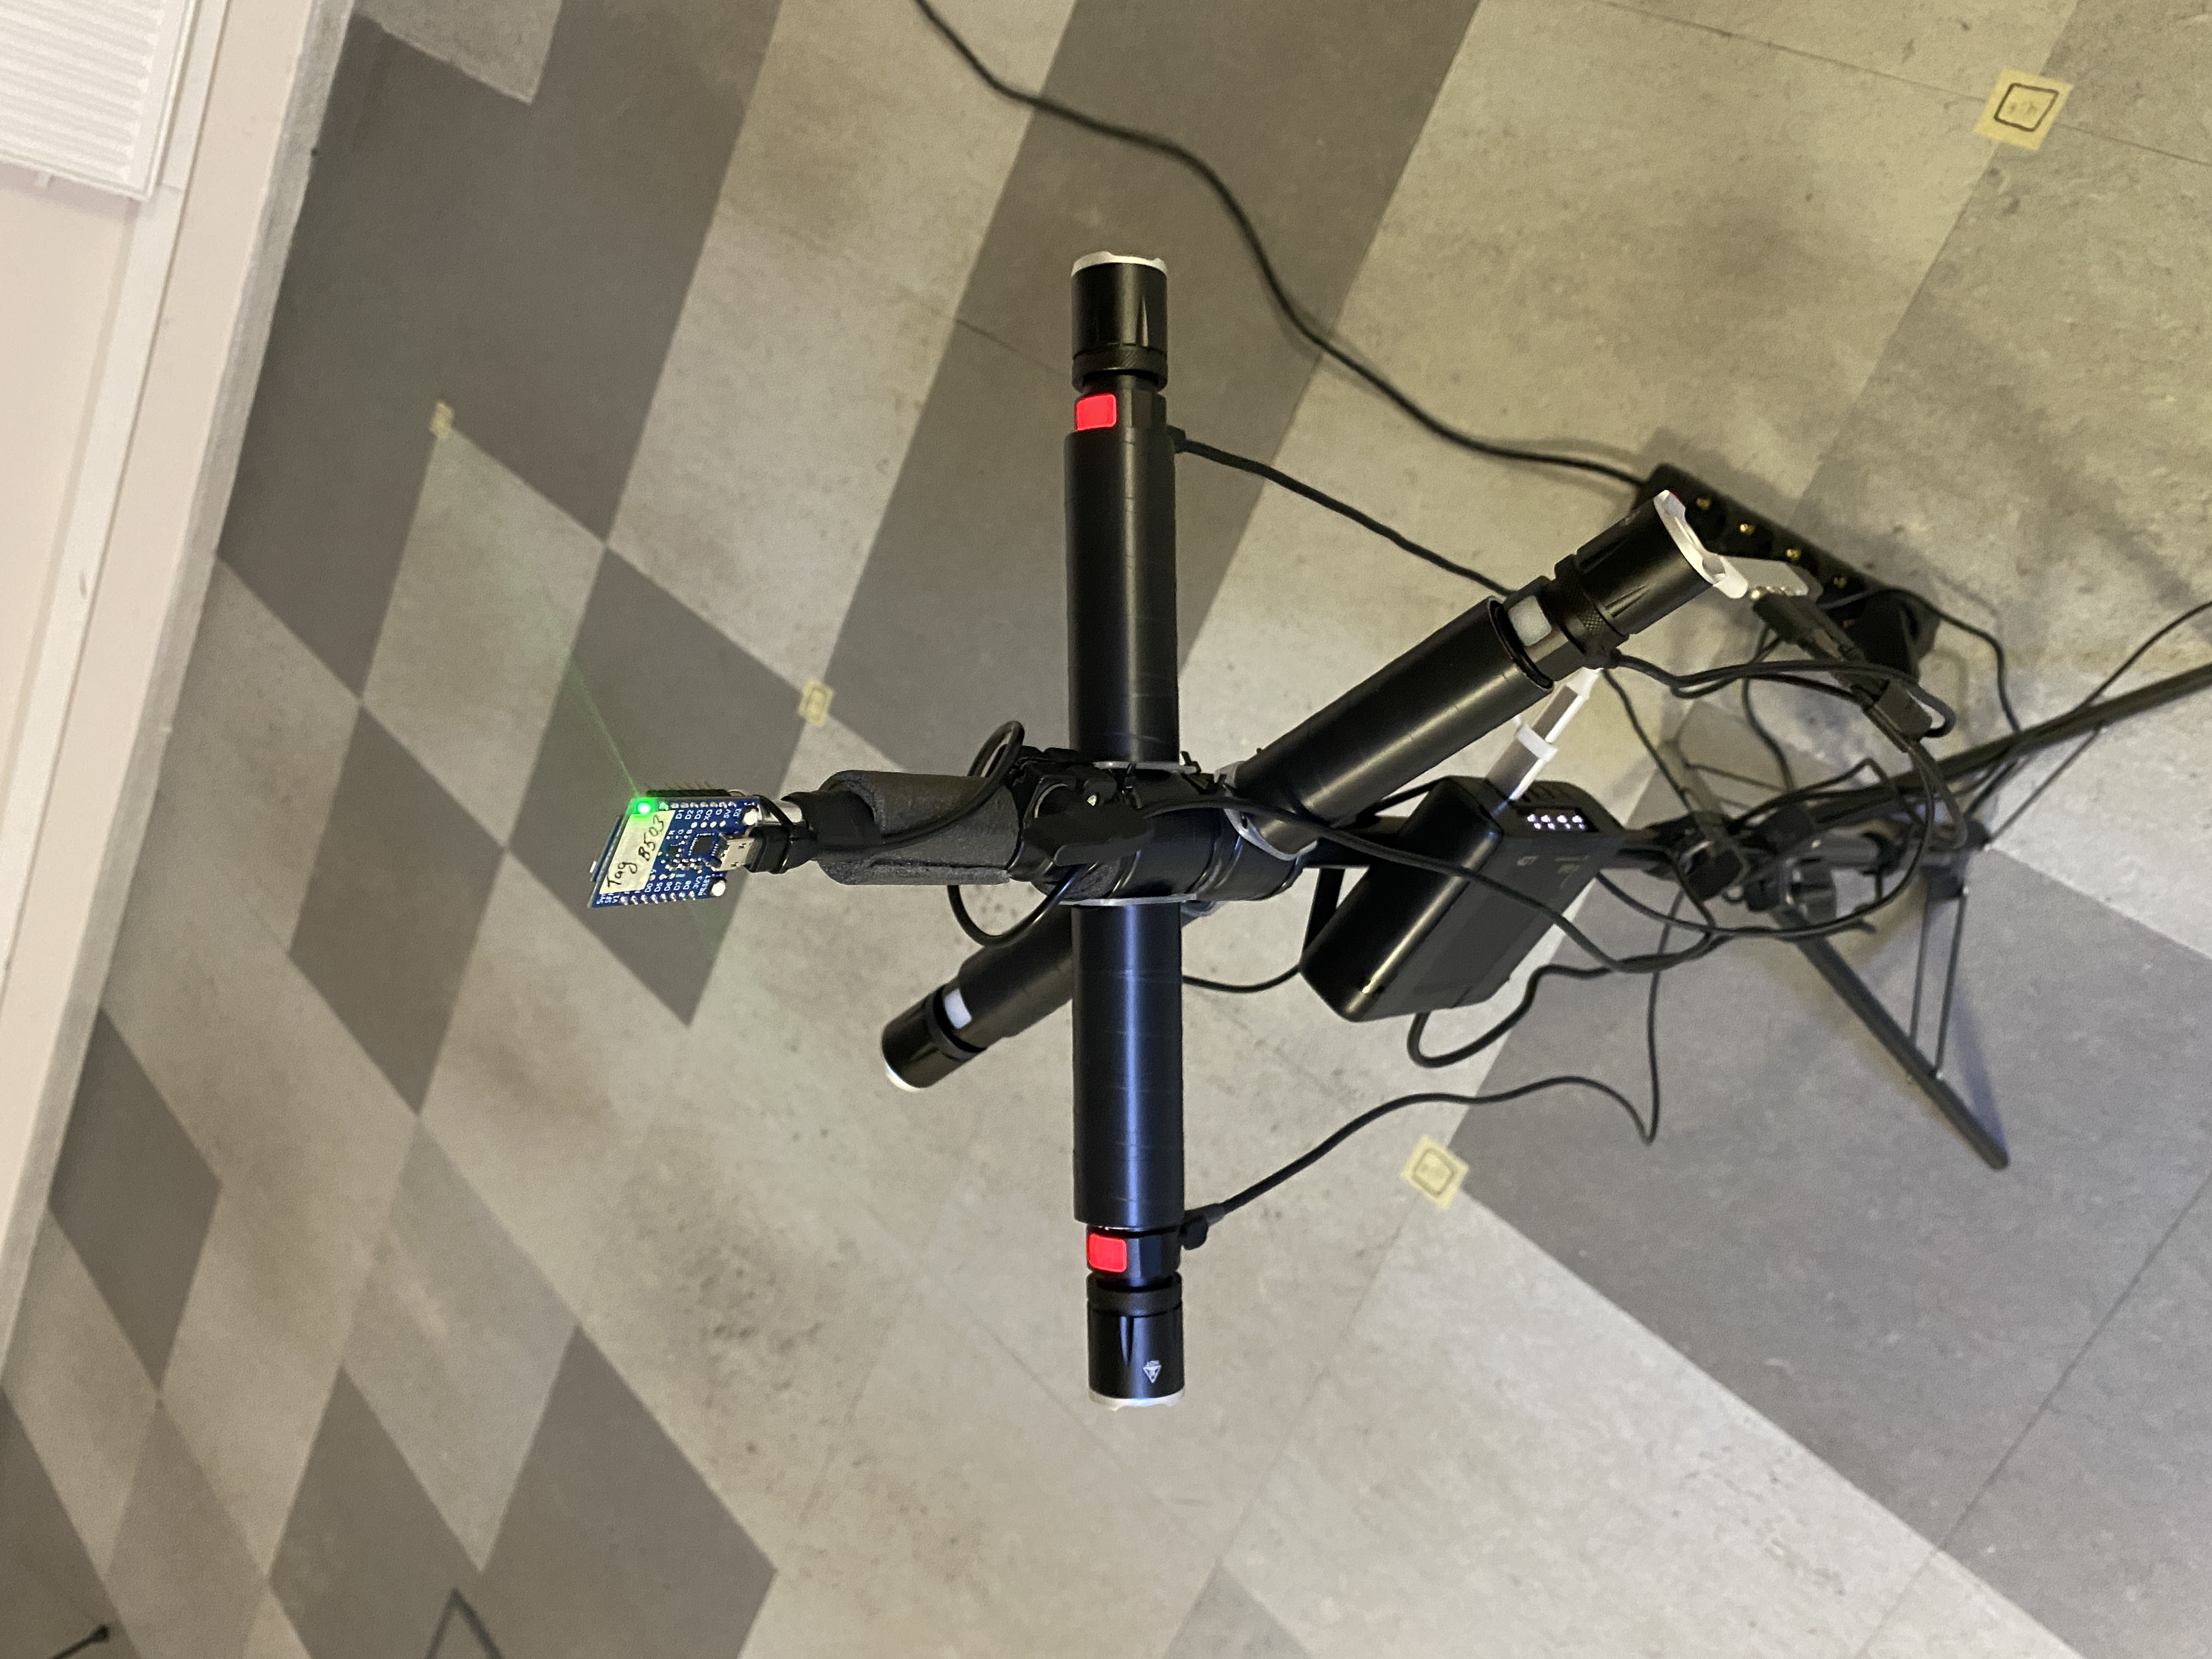
\includegraphics[height=6.5cm]{Figures/methodology/tag.png}
        \label{fig:tag}
    }
    \caption{Setup used for \textit{RangeCIR} dataset collection.}
    \label{fig:dataset_setup}
\end{figure}

To the best of the author's knowledge, no publicly available datasets are compatible with the hardware used in this study. Therefore, a custom dataset was acquired through a controlled experimental campaign.

\begin{figure}[tbh]
\hspace*{-20pt} % To align the legend of the figure with caption, looks more appealing
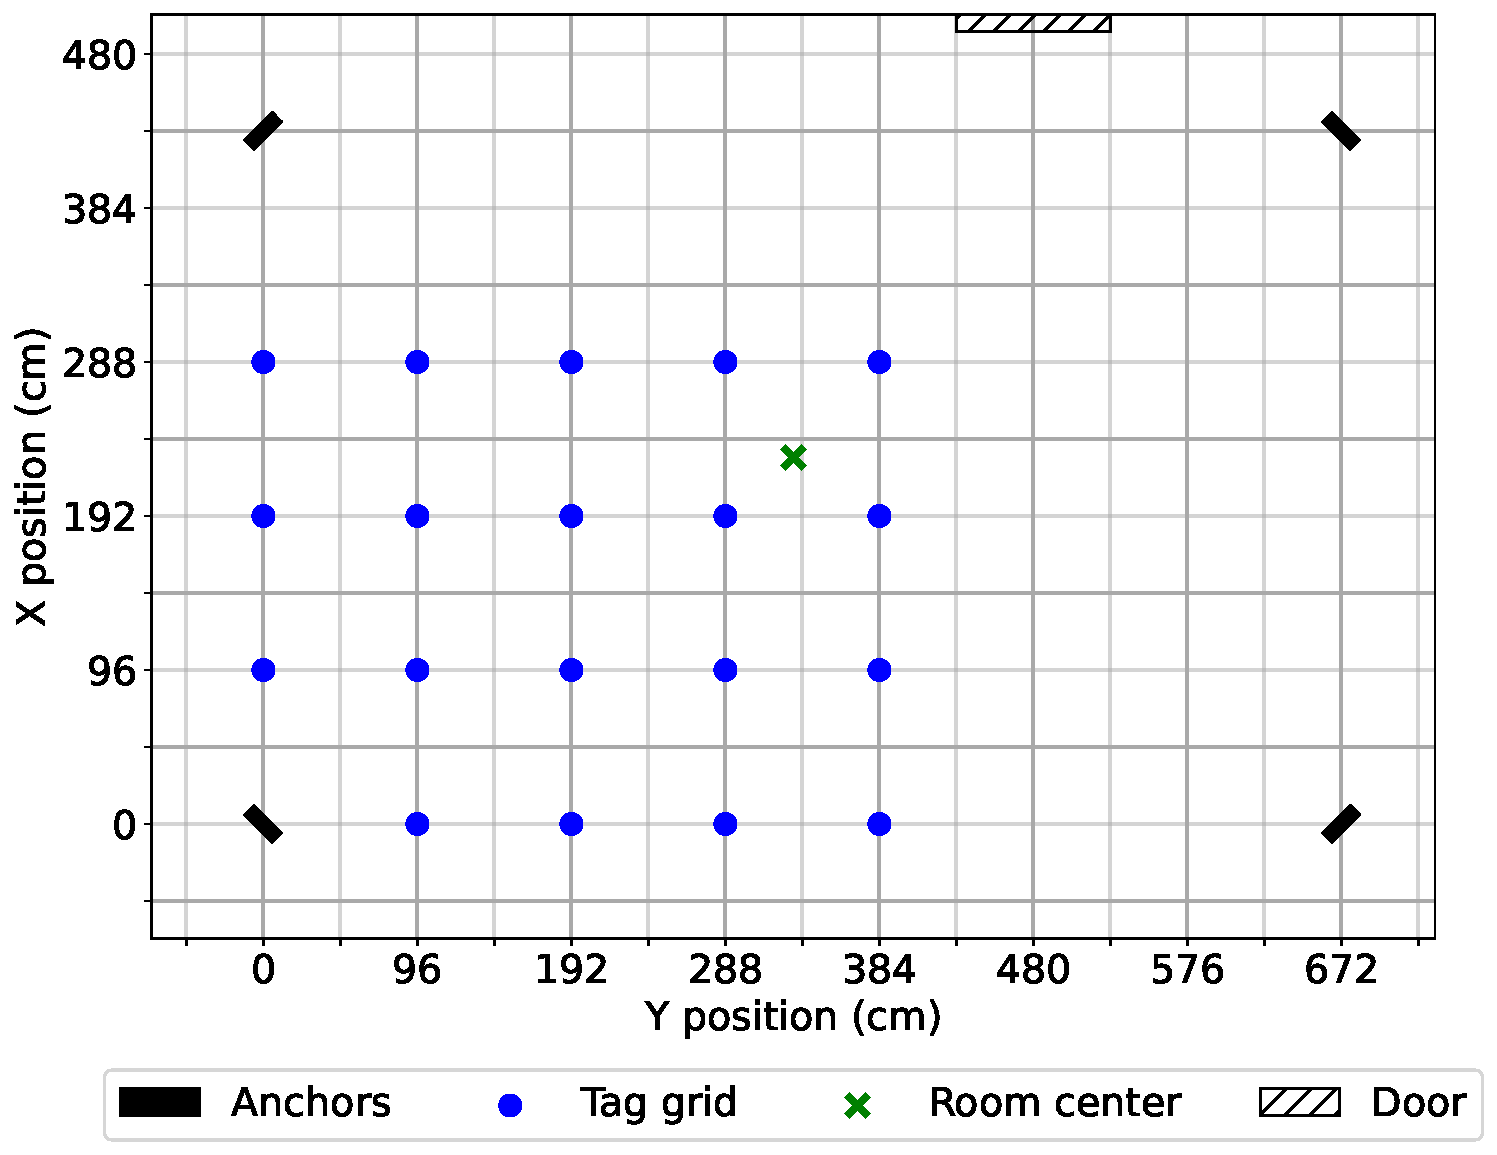
\includegraphics[width=0.75\textwidth]{Figures/methodology/dataset_scheme.pdf}
\centering
\caption{Schematic of the dataset collection setup.}
\label{fig:exp_topology}
\end{figure}

Measurements were carried out using the SynchronicIT SFM10-DEV development board\footnote{\url{https://synchronicit.nl/hardware?topic=SFM10-DEV}}, based on the SFM10-MOD, an IEEE 802.15.4z-compliant IR-UWB module built around the NXP Trimension OL23D0 chipset. The radio was configured to operate on UWB channel 5 (central frequency of~\SI{6489.6}{\mega\hertz}, bandwidth of \SI{499.2}{\mega\hertz}). The SHR preamble length was set to 32 symbols. Ranging and CIR acquisition were powered by custom firmware discussed in \autoref{ranging_system}. 

The data collection took place in an approximately $6 \times 8$~\si{\meter} university classroom. Four fixed anchors were placed at the room's corners, while a single tag was moved along a predefined grid confined to one quadrant of the room. This configuration was chosen to reduce the data collection efforts and time by minimizing the spatial symmetry duplications without loss of generality. At each grid point, the tag was rotated around its vertical axis through a~\SI{360}{\degree} sweep to capture variability in directional antenna characteristics, while its location was kept constant. All devices were mounted vertically at a height of~\SI{120}{\centi\metre}, taking antenna polarization into account. \autoref{fig:dataset_setup} shows the data collection environment and setup, while~\autoref{fig:exp_topology} illustrates the layout, including anchor placements and the tag’s movement grid.

Distance measurements were acquired using the ADS-TWR method, with approximately 50,000 samples collected per tag position at a sampling frequency of~\SI{270}{\hertz}. Each measurement recorded both the estimated distance and the corresponding CIR associated with the Final packet of the TWR protocol (see \autoref{theory:twr} for further details on TWR). A total of 136 CIR samples were captured per measurement, comprising 8 samples preceding and 127 samples following the first path. This sampling strategy was determined empirically to balance data compactness with the need to capture sufficient environmental detail for subsequent error correction.

To model realistic NLoS conditions, dynamic human obstructions were introduced by instructing five volunteers to move pseudo-randomly throughout the room, intermittently blocking the direct paths between the transceivers. Given the inherent unpredictability of such movements, manual labeling of each measurement as LoS or NLoS was infeasible. However, reliable annotation is essential for maintaining dataset balance, enabling context-aware analysis, and supporting future studies focused on classification tasks. An automated optical tracking system was therefore employed to determine LoS/NLoS conditions during data collection. A comprehensive description of the tracking system implementation is presented in \autoref{tracking_system}.

To ensure data quality and balance, we developed a custom real-time graphical user interface (GUI). During the data collection process, the GUI was projected on the wall to be clearly visible to all participants and displayed: live distance measurements, system status for each anchor, the current ratio of NLoS to LoS measurements, and the cumulative count of recorded samples. Volunteers were guided to maintain an NLoS measurement ratio exceeding \SI{50}{\percent}, thereby ensuring a dataset with sufficient variability for effective model training.

The known locations of the tag and anchors were subsequently translated into the ground truth distances, and individual measurement sessions were aggregated accordingly. To this end, the resulting dataset includes estimated and ground truth distances, LoS/NLoS labels, and synchronized CIR measurements. This dataset, referred to as \textit{RangeCIR}, has been made publicly available to support reproducibility and to promote further research on NLoS error mitigation and channel classification~\cite{yaroshevych_2025_rangecir}.

\section{Proposed IPS pipeline}

\begin{figure}[tbh]
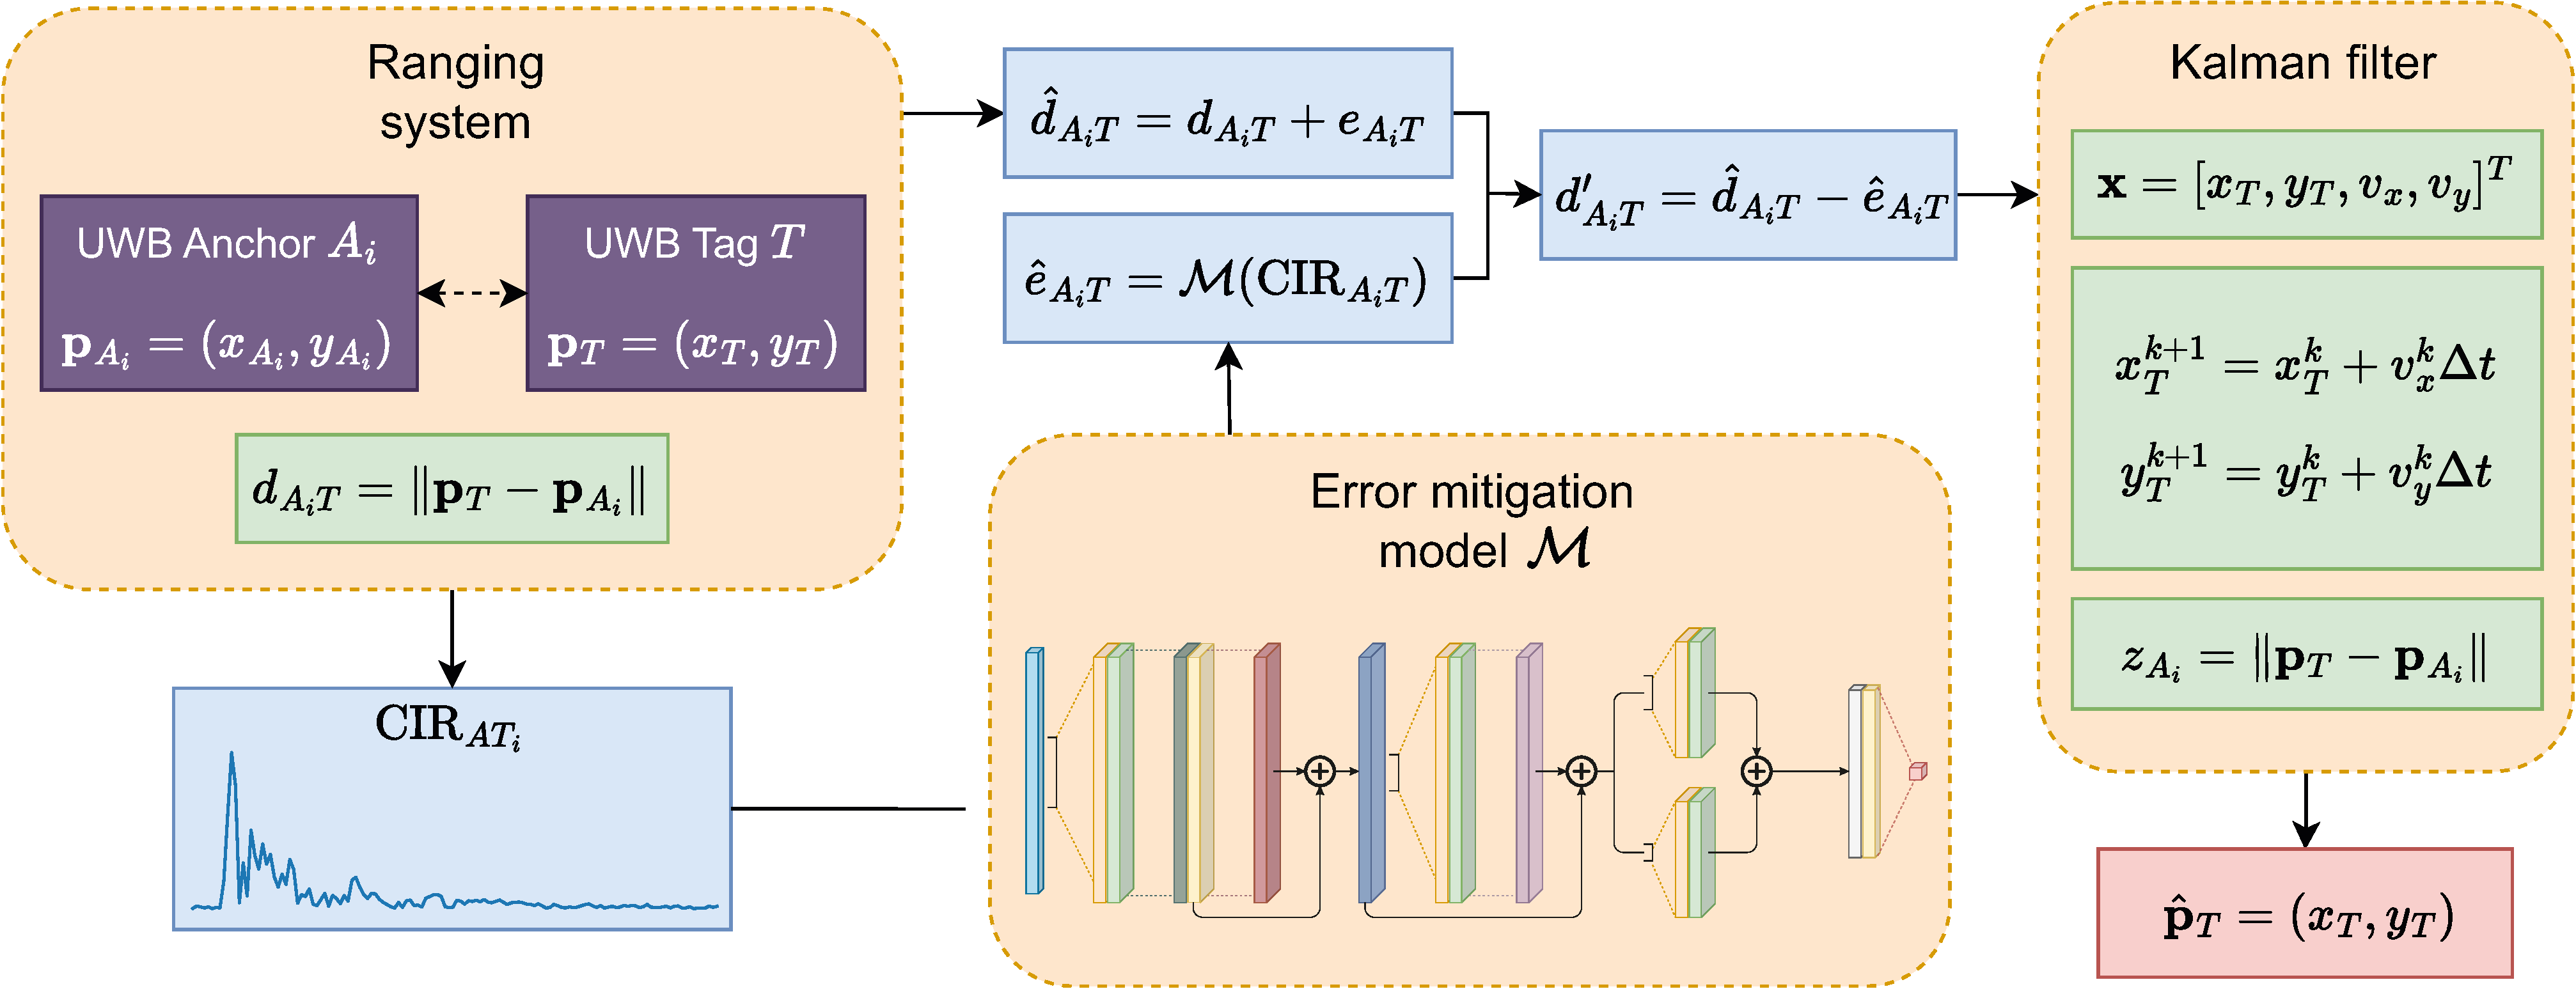
\includegraphics[width=\textwidth]{Figures/methodology/pipeline.pdf}
\centering
\caption{The proposed IPS pipeline.}
\label{fig:pipeline}
\end{figure}

The pipeline of the proposed IPS is depicted in \autoref{fig:pipeline}. The following part of this section will separately discuss each of its three major modules: 

\begin{enumerate}
    \item Ranging system;
    \item Error mitigation model;
    \item Kalman filter.
\end{enumerate}

\subsection{Ranging system}\label{ranging_system}

\paragraph{Architecture.}

\begin{figure}[tbh]
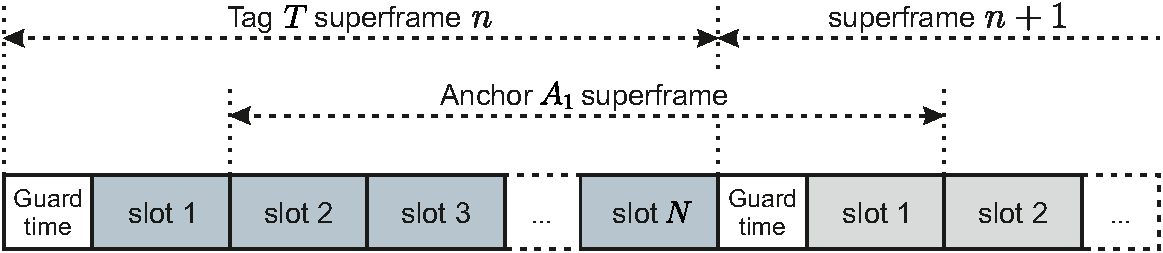
\includegraphics[width=0.85\textwidth]{Figures/methodology/superframe_structure.pdf}
\centering
\caption{Superframe structure.}
\label{fig:superframe}
\end{figure}

\begin{figure}[tbh]
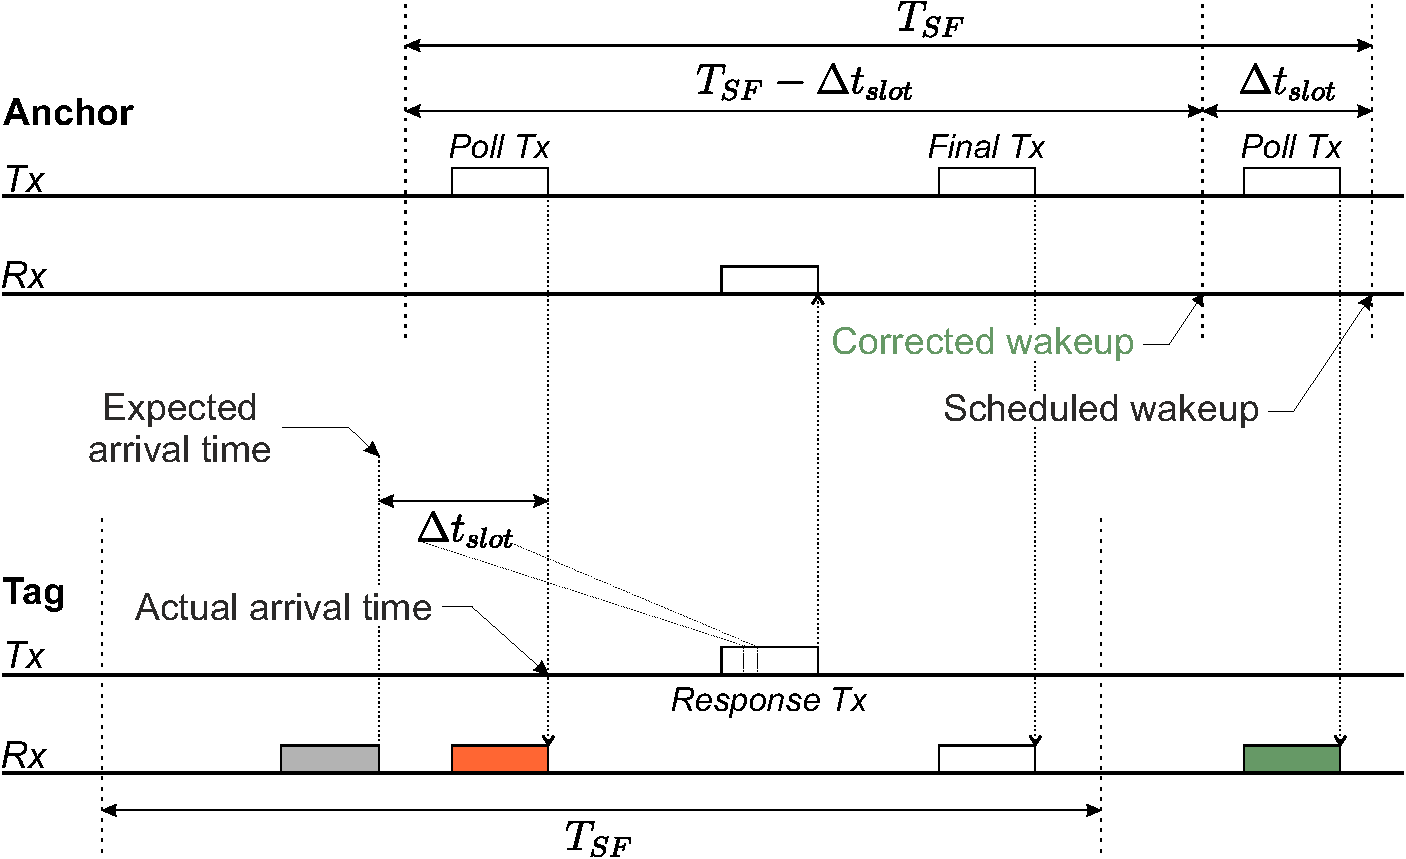
\includegraphics[width=0.75\textwidth]{Figures/methodology/slot_correction.pdf}
\centering
\caption{Slot correction mechanism.}
\label{fig:slot_correction}
\end{figure}

The ranging system forms the foundational layer of the proposed IPS pipeline, enabling continuous acquisition of inter-device distances used for localization. The system architecture differentiates between two roles: \textit{anchors}, which are statically deployed at known locations $\mathbf{p}_{A_i} = (x_{A_i}, y_{A_i}) \in \mathbb{R}^2$, and a \textit{tag}, which is mobile and continuously performs distance measurements relative to each anchor with unknown position $\mathbf{p}_T = (x_T, y_T) \in \mathbb{R}^2$ to be estimated. 

All devices operate under a custom TDMA protocol\footnote{The design of the TDMA protocol and the slot correction mechanism used in this study was inspired by Qorvo's UWB software stack, which implements similar synchronization strategies: \url{https://www.qorvo.com/products/d/da007992}.} (refer to \autoref{tdma} for background). Each ranging operation is executed within a so-called TDMA \emph{superframe} structure of duration $T_{SF}$, subdivided into $N$ non-overlapping slots, each uniquely assigned to an anchor. This structure is shown in \autoref{fig:superframe}. At the start of every superframe, all devices are awakened via a timer interrupt. Notably, each device maintains its own local superframe timing, derived from its internal clock. During its assigned slot, the anchor initiates the transaction by broadcasting a \emph{Poll} message. Upon reception, the tag responds with a \emph{Response} message, embedding timing feedback, which will be detailed later. The anchor finalizes the transaction with a delayed transmission of the \emph{Final} message, which includes all timing information necessary for the tag to compute the ToF. This transaction follows the ADS-TWR protocol, discussed in \autoref{adstwr}, and enables the tag $T$ to estimate the raw range $\hat{d}_{A_i,T}$ between itself and each anchor $A_i$:
\begin{equation}
\hat{d}_{A_i,T} = d_{A_i,T} + e_{A_i,T},\label{eq:raw_range}
\end{equation}
where $e_{A_i,T}$ denotes the aggregated ranging error component, which is consequently mitigated using the CIR-driven error mitigation model, and $d_{A_i,T}$ is the true geometric distance between the tag and the $i$-th anchor, defined as the Euclidean norm:
\begin{equation} 
d_{A_i,T} = \left\| \mathbf{p}_T - \mathbf{p}_{A_i} \right\|.\label{eq:true_distance} 
\end{equation}

To maintain TDMA slot integrity, precise temporal alignment between anchors is essential. To this end, the tag computes a \textit{slot correction} value $\Delta t_{\text{slot}}$ upon reception of each Poll message, quantifying the offset between its expected and actual arrival times relative to the start of the superframe. This correction term is then embedded in the Response message and fed back to the anchor, which uses it to dynamically adjust the scheduling of subsequent superframes, thereby preserving tight synchronization. \autoref{fig:slot_correction} illustrates this mechanism in detail.

The source code implementing the ranging system firmware is publicly available on GitHub\footnote{\url{https://github.com/andylvua/SFM10-DEV-TWR}}, supporting reproducibility and further development.

\paragraph{CIR acquisition.}

A core feature of the proposed system is the ability to extract and transmit the channel impulse response $\text{CIR}_{A_i,T}$ associated with each ranging transaction, which enables subsequent error correction with the proposed model, as illustrated in~\autoref{fig:pipeline}. Depending on the device configuration, CIR data may be acquired either by the tag upon reception of the Final message, or by the anchor upon reception of the Response message. Each CIR accumulator contains up to 255 samples, with each sample comprising a 2-byte real and a 2-byte imaginary component, resulting in a raw data footprint of 4 bytes per sample.

However, our analysis reveals that approximately \SI{93}{\percent} of the differences between sequential raw CIR values (real and imaginary parts are treated as separate sequences and differenced individually) can be efficiently represented using only 1 byte. Therefore, to increase the data transmission rate and subsequently improve the ranging frequency, the system implements a 7-bit adaptive delta-encoding scheme for CIR compression. The encoding proceeds as follows:

\begin{enumerate} 
    \item for each CIR sample component (real or imaginary), the difference $\Delta x = x_i - x_{i-1}$ is computed;
    \item if $|\Delta x| \leq 63$, the delta is encoded in a single byte, using low 7 bits for value, and the most significant bit as a continuation flag (set to 0);
    \item if $|\Delta x| > 63$, a two-byte representation is used. The first byte contains the high 7 bits of the delta, with the continuation flag set to 1. The second byte stores the remaining 8 bits. 
\end{enumerate} 
As a result, the effective measurement frequency is increased by over \SI{20}{\percent} compared to transmitting raw samples, as observed for CIR sequences containing 136 samples. Both the encoding on the device side and the decoding on the host side impose negligible computational overhead.

\subsection{Error mitigation model}

As discussed in \autoref{error_sources}, raw distance measurements are inherently affected by various sources of error, including multipath propagation and NLoS conditions. These conditions introduce error $e_{A_i,T}$ between the true distance $d_{A_i,T}$ and the measured distance $\hat{d}_{A_i,T}$ (\autoref{eq:raw_range}). To improve localization accuracy, it is imperative to estimate and correct for this error component prior to position estimation. 

To this end, we employ a learning-based error mitigation module $\mathcal{M}$ that is used to infer the error estimate $\hat{e}_{A_i,T}$ as a function of the channel impulse response (see \autoref{cir_theory} for a detailed discussion of CIR fundamentals), denoted $\text{CIR}_{A_iT}$:
\begin{equation}
    \hat{e}_{A_i,T} = \mathcal{M}(\text{CIR}_{A_iT}),
\end{equation}
which is then subtracted from the raw measurement to obtain a corrected range:
\begin{equation}
    d'_{A_i,T} = \hat{d}_{A_i,T} - \hat{e}_{A_i,T}.
\end{equation}

The corrected range $d'_{A_i,T}$ later serves as the input to the proposed Kalman filter, enabling more accurate and robust state estimation. As mentioned before, \autoref{fig:pipeline} illustrates this proposed pipeline.

\paragraph{Foundational model.}

The proposed model $\mathcal{M}$ builds upon the \emph{REMNet (Range Error Mitigation Network)}, deep residual architecture introduced by Simone Angarano et al. in~\cite{Simone2021UWB}, which demonstrated the feasibility of learning ranging errors from CIR. In the original formulation of REMNet architecture, the input CIR vector of length $K$, is first transformed through a 1D convolutional layer that extracts $F$ low-level features. Unless otherwise specified, all convolutional and fully connected layers are followed by ReLU activations. This initial representation is passed through a stack of $N$ identical residual reduction modules (RRMs), each performing two main operations: residual feature transformation and temporal dimensionality reduction. 

\begin{figure}[thb]
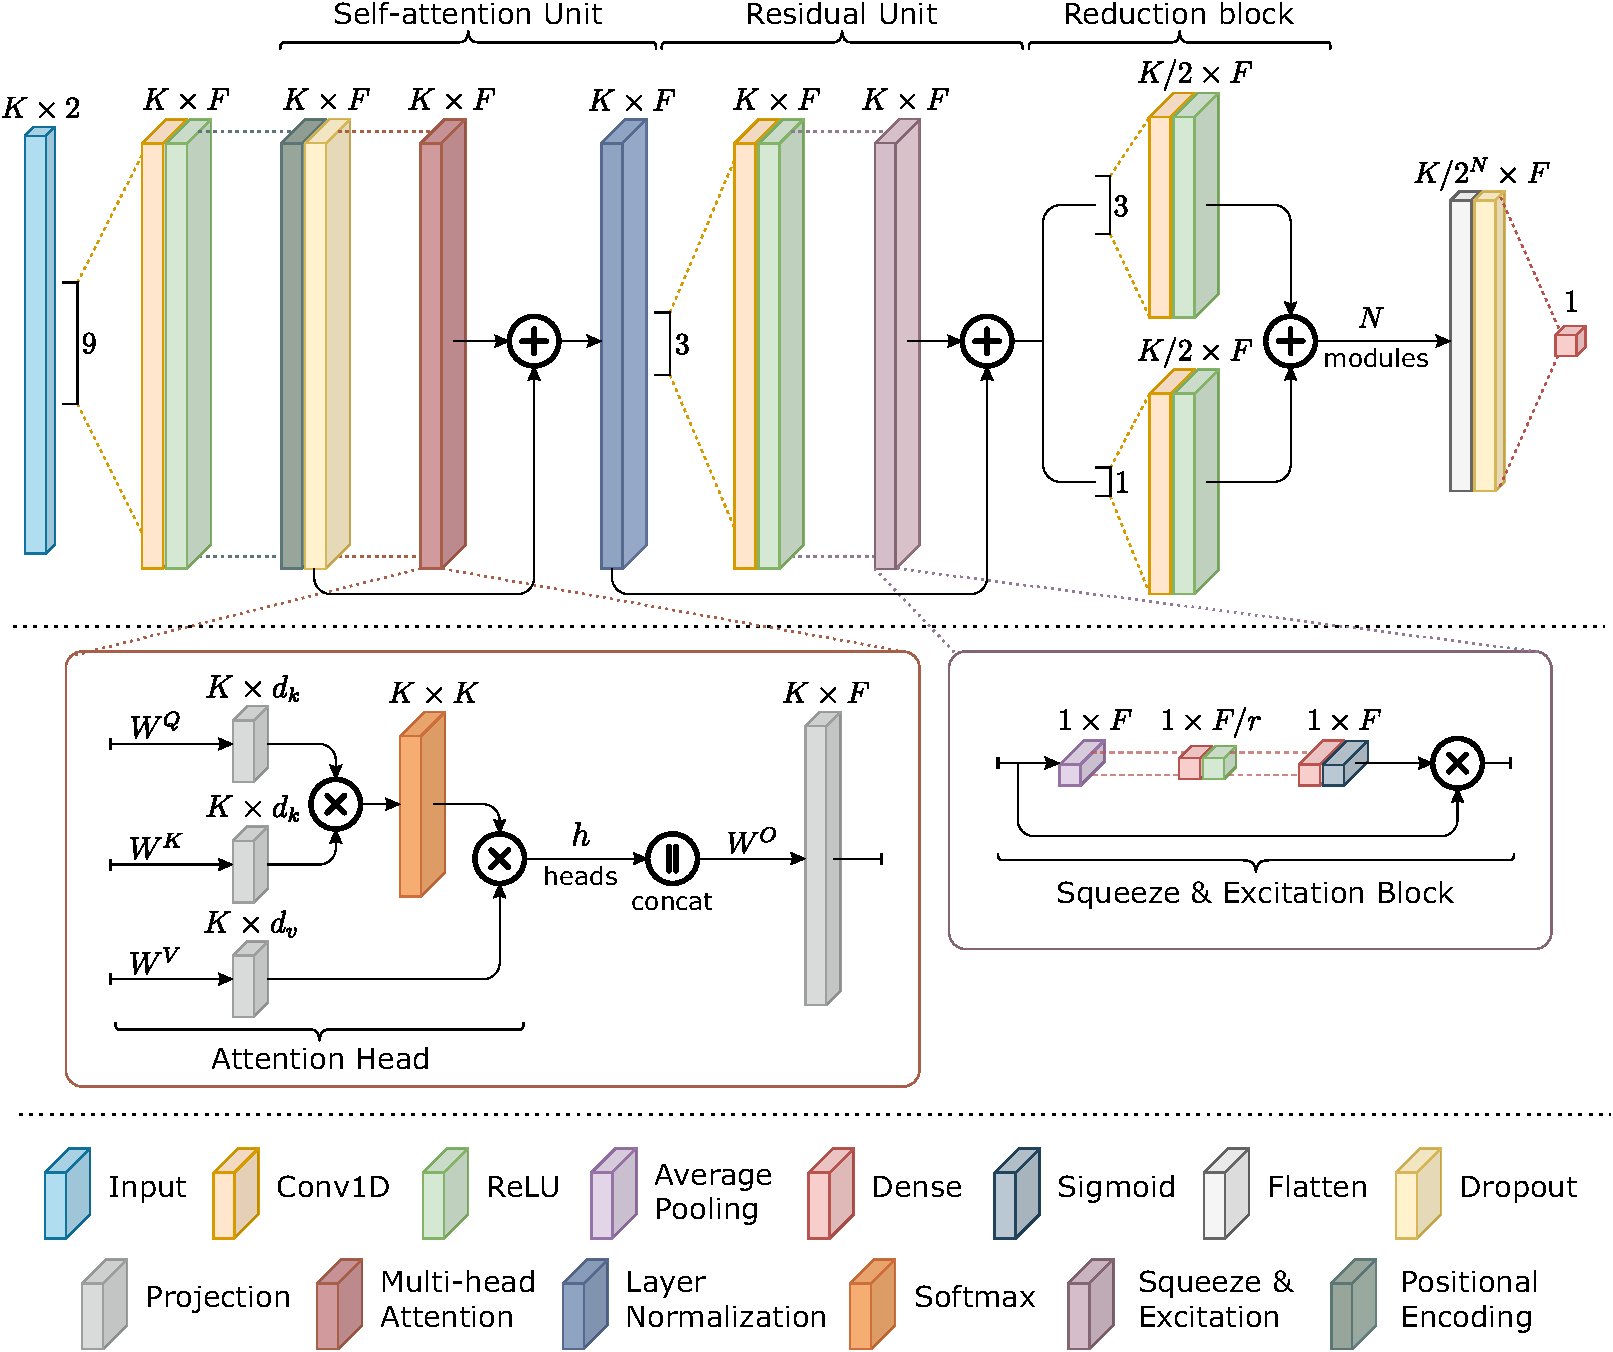
\includegraphics[width=\textwidth]{Figures/methodology/remnet_compat.pdf}
\centering
\caption[Proposed A-REMNet architecture.]{Proposed A-REMNet architecture. Figure is adapted from Simone Angarano et al.~\cite{Simone2021UWB}, with permission from the authors.}
\label{fig:architecture}
\end{figure}

Each RRM can be functionally described as:
\begin{equation}
    \text{RRM}(\mathbf{X}) = \text{Red}(\text{Res}(\mathbf{X})),
\end{equation}
where $\mathbf{X} \in \mathbb{R}^{K \times F}$ is the input tensor, $\text{Res}(\cdot)$ denotes a residual transformation unit, and $\text{Red}(\cdot)$ is a dimensionality reduction block. The residual unit is defined as:
\begin{equation}
    \text{Res}(\mathbf{X}) = \text{SE}(\text{Conv1D}(\mathbf{X})) + \mathbf{X},
\end{equation}
where $\text{Conv1D}$ denotes a 1D convolution, and $\text{SE}(\cdot)$ is a squeeze-and-excitation block. The SE block introduces channel-wise attention by using global average pooling to extract channel descriptors, followed by a two-layer bottleneck that produces scaling factors for self-gating, i.e., reweighting each channel by a value derived from itself. Given an intermediate feature map $ \mathbf{X} \in \mathbb{R}^{K \times F} $, the SE operation is defined as:
\begin{equation}
    \text{SE}(\mathbf{X}) = \mathbf{X} \cdot \boldsymbol{\alpha}, \qquad \boldsymbol{\alpha} = \text{FC}_2\left(\text{FC}_1(\text{GAP}(\mathbf{X}))\right),
\end{equation}
where $\text{GAP}(x) = \frac{1}{K} \sum_{k=1}^{K} x_{k,:}$ performs global average pooling over the temporal axis, and $\text{FC}_1: \mathbb{R}^{1 \times F} \rightarrow \mathbb{R}^{1 \times F/r}$, $\text{FC}_2: \mathbb{R}^{1 \times F/r} \rightarrow \mathbb{R}^{1 \times F}$ are fully connected layers with ReLU and sigmoid activations, respectively. Here, $r$ is the reduction ratio controlling the compression rate in the bottleneck. The resulting scaling vector $\boldsymbol{\alpha} \in \mathbb{R}^{1 \times F}$ modulates the importance of each feature channel.

Following the residual transformation, the RRM performs temporal downsampling through the reduction block, which comprises two parallel strided convolutional branches:
\begin{equation}
    \text{Red}(\mathbf{X}) = \text{Conv1D}_1(\mathbf{X}) + \text{Conv1D}_2(\mathbf{X}),
\end{equation}
where $\text{Conv1D}_1$ and $\text{Conv1D}_2$ utilize different kernel sizes to capture both coarse- and fine-grained features. Each branch produces a feature map in $\mathbb{R}^{K/2 \times F}$, preserving the feature dimensionality while reducing the temporal resolution.

After passing through $N$ successive RRMs, the resulting feature tensor lies in $\mathbb{R}^{K / 2^N \times F}$. This tensor is then flattened and passed through a dropout layer to mitigate overfitting, followed by a fully connected layer with linear activation that outputs the final regressive error estimate $\hat{e}_{A_i,T}$.

\paragraph{Proposed \emph{A-REMNet} approach.}
We introduce two key enhancements designed to improve the model's representational capacity and performance. First, in contrast to the original architecture, which discards CIR phase information by utilizing only its magnitude, we retain the full complex-valued CIR in a two-channel format (separating real and imaginary components), i.e.,
\begin{equation}
    \text{CIR}_{A_iT} \in \mathbb{R}^{K \times 2}.
\end{equation}
We believe this allows the network to learn richer signal characteristics that would otherwise be discarded if only the magnitude was employed.

Second, and more critically, we augment the architecture with a temporal self-attention unit, yielding the proposed \emph{Attention-enhanced Range Error Mitigation Network (A-REMNet)}, illustrated in \autoref{fig:architecture}. The proposed unit $\text{Att}(\cdot)$ is embedded directly in RRM before the residual unit, modifying the RRM as:
\begin{equation}
    \text{RRM}(\mathbf{X}) = \text{Red}(\text{Res}(\text{Att}(\mathbf{X}))).
\end{equation}
Unlike the SE block, the self-attention module operates along the temporal dimension of the CIR, allowing the model to capture long-range dependencies that conventional convolutional kernels may overlook. Inspired by the Transformer architecture introduced in~\cite{attention}, we adopt a multi-head self-attention (MHSA) mechanism to enable the model to attend to multiple subspaces of the temporal sequence in parallel, followed by a layer normalization on the residual branch to stabilize the learning process:
\begin{equation}
    \text{Att}(\mathbf{X}) = \text{LayerNorm}(\text{MHSA}(\mathbf{X}) + \mathbf{X}).
\end{equation}

Formally, given an input tensor $\mathbf{X} \in \mathbb{R}^{K \times F}$ at a hidden layer, where $F$ denotes the feature embedding dimension, the multi-head self-attention mechanism computes attention outputs as:
\begin{equation}
    \text{MHSA}(\mathbf{X}) = \text{Concat}(\text{head}_1, \dots, \text{head}_h) W^O,
\end{equation}
where each attention head is given by:
\begin{equation}
    \text{head}_i = \text{Attention}(\mathbf{X} W_i^Q, \mathbf{X} W_i^K, \mathbf{X} W_i^V),
\end{equation}
and the scaled dot-product attention mechanism is defined as:
\begin{equation}
    \text{Attention}(\mathbf{Q}, \mathbf{K}, \mathbf{V}) = \text{softmax}\left( \frac{\mathbf{Q} \mathbf{K}^\top}{\sqrt{d_k}} \right) \mathbf{V},
\end{equation}
where $h$ is the number of heads, and $W_i^Q \in \mathbb{R}^{F \times d_k}$, $W_i^K \in \mathbb{R}^{F \times d_k}$, $W_i^V \in \mathbb{R}^{F \times d_v}$, $W^O \in \mathbb{R}^{hd_v \times F}$ are learned projection matrices. Here, $d_k = d_v = F/h$ is the dimension of each attention head. This mechanism enables dynamic weighting of temporal features, targeted at making the model particularly effective in identifying non-local patterns and multipath structures indicative of NLoS conditions.

To provide the attention mechanism with information about the temporal ordering of CIR taps, we incorporate learnable positional encoding, following an approach similar to that used in many Transformer models~\cite{2019-bert, 2022-simple-yet}. A distinct embedding vector is assigned to each temporal index, and these vectors are added to the input features prior to the attention operation. For an intermediate feature map $\mathbf{X} \in \mathbb{R}^{K \times F}$, the position-augmented representation is computed as:
\begin{equation}
    \mathbf{X}' = \text{Dropout}(\mathbf{X} + \mathbf{P}),
\end{equation}
where $\mathbf{P} \in \mathbb{R}^{K \times F}$ is a learnable positional embedding matrix, and dropout is applied to prevent overfitting. This encoding enables the model to associate temporal positions with specific signal characteristics, which is particularly relevant given the structured nature of CIRs, where early and late taps often represent different propagation behaviors.

\subsection{Kalman filter}

As previously outlined, following the mitigation of ranging errors, the final stage of the proposed pipeline (\autoref{fig:pipeline}) performs sequential fusion and smoothing of the corrected measurements to estimate the tag's trajectory over time by applying an Extended Kalman Filter. This section details the implementation of the proposed EKF, building upon the theoretical background presented in \autoref{kalman_theory}.

The objective is to estimate the two-dimensional position and velocity of the mobile tag, denoted as the state vector:
\begin{equation}
        \mathbf{x}_k = [x_k, y_k, v_{x_k}, v_{y_k}]^\top \in \mathbb{R}^4,
\end{equation}
where $(x_k, y_k)$ and $(v_{x_k}, v_{y_k})$ represent the position and velocity components at time step $k$, respectively.

\paragraph{State transition model.}

Assuming constant velocity motion with small Gaussian perturbations, the dynamics of the tag are modeled by a linear time-invariant system:
\begin{equation}
    \mathbf{x}_k = \mathbf{F}_k \mathbf{x}_{k-1} + \mathbf{w}_{k-1},
\end{equation}
where the state transition matrix $\mathbf{F}_k$ incorporates the time increment $\Delta t$:
\begin{equation}
    \mathbf{F}_k =
    \begin{bmatrix}
        1 & 0 & \Delta t & 0 \\
        0 & 1 & 0 & \Delta t \\
        0 & 0 & 1 & 0 \\
        0 & 0 & 0 & 1
    \end{bmatrix},
\end{equation}
and $\mathbf{w}_{k-1} \sim \mathcal{N}(0, \mathbf{Q})$ is the process noise. The process noise covariance $\mathbf{Q}$ is modeled as a scaled identity matrix to reflect independent perturbations in all dimensions:
\begin{equation}
    \mathbf{Q} = \sigma^2_q \mathbf{I}_4,
\end{equation}
where $\sigma^2_q$ is the process noise variance hyperparameter.

\paragraph{Observation model.}

Each measurement at time step $k$ corresponds to a corrected range $d'_{A_i,T}$ between the tag $T$ and an anchor $A_i$ with known coordinates $\mathbf{p}_{A_i} = (x_{A_i}, y_{A_i})$. This relationship is governed by the nonlinear measurement function:
\begin{equation}
    z_k = h(\mathbf{x}_k) + v_k = \sqrt{(x_k - x_{A_i})^2 + (y_k - y_{A_i})^2} + v_k,
\end{equation}
where $v_k \sim \mathcal{N}(0, \mathbf{R}_k)$ is the measurement noise with variance $\mathbf{R}_k$. We note that only one anchor contributes a range measurement at each discrete time step, due to the TDMA scheduling structure (see \autoref{ranging_system} for the details).

The observation model is linearized around the current predicted state via its Jacobian $\mathbf{H}_k$:
\begin{equation}
\mathbf{H}_k = \frac{\partial h}{\partial \mathbf{x}} \big|_{\hat{\mathbf{x}}_k^-} = 
\begin{bmatrix}
    \dfrac{\hat{x}_k^- - x_{A_i}}{h(\hat{\mathbf{x}}_k^-)} &
    \dfrac{\hat{y}_k^- - y_{A_i}}{h(\hat{\mathbf{x}}_k^-)} &
    0 & 0
\end{bmatrix}.
\end{equation}

Prediction and update steps then follow the standard formulation described in \autoref{kalman_theory}.

% At each time step, the EKF performs the standard predict and update steps:
%% Moved to theoretical background

% \emph{Prediction:}
% \begin{align}
%     \hat{\mathbf{x}}_k^- &= \mathbf{F}_k \hat{\mathbf{x}}_{k-1} \\
%     \mathbf{P}_k^- &= \mathbf{F}_k \mathbf{P}_{k-1} \mathbf{F}_k^\top + \mathbf{Q}_k,
% \end{align}

% \emph{Update:}
% \begin{align}
%     \mathbf{K}_k &= \mathbf{P}_k^- \mathbf{H}_k^\top \left( \mathbf{H}_k \mathbf{P}_k^- \mathbf{H}_k^\top + R_k \right)^{-1} \\
%     \hat{\mathbf{x}}_k &= \hat{\mathbf{x}}_k^- + \mathbf{K}_k \left(z_k - h(\hat{\mathbf{x}}_k^-)\right) \\
%     \mathbf{P}_k &= \left(\mathbf{I} - \mathbf{K}_k \mathbf{H}_k\right) \mathbf{P}_k^-,
% \end{align}
% where $\mathbf{K}_k$ is the Kalman gain, $\hat{\mathbf{x}}_k$ is the posterior state estimate, and $\mathbf{P}_k$ is the corresponding covariance.
 
\chapter{Experiments and results}

\section{Ranging system}

\begin{figure}[tbh]
    \centering
    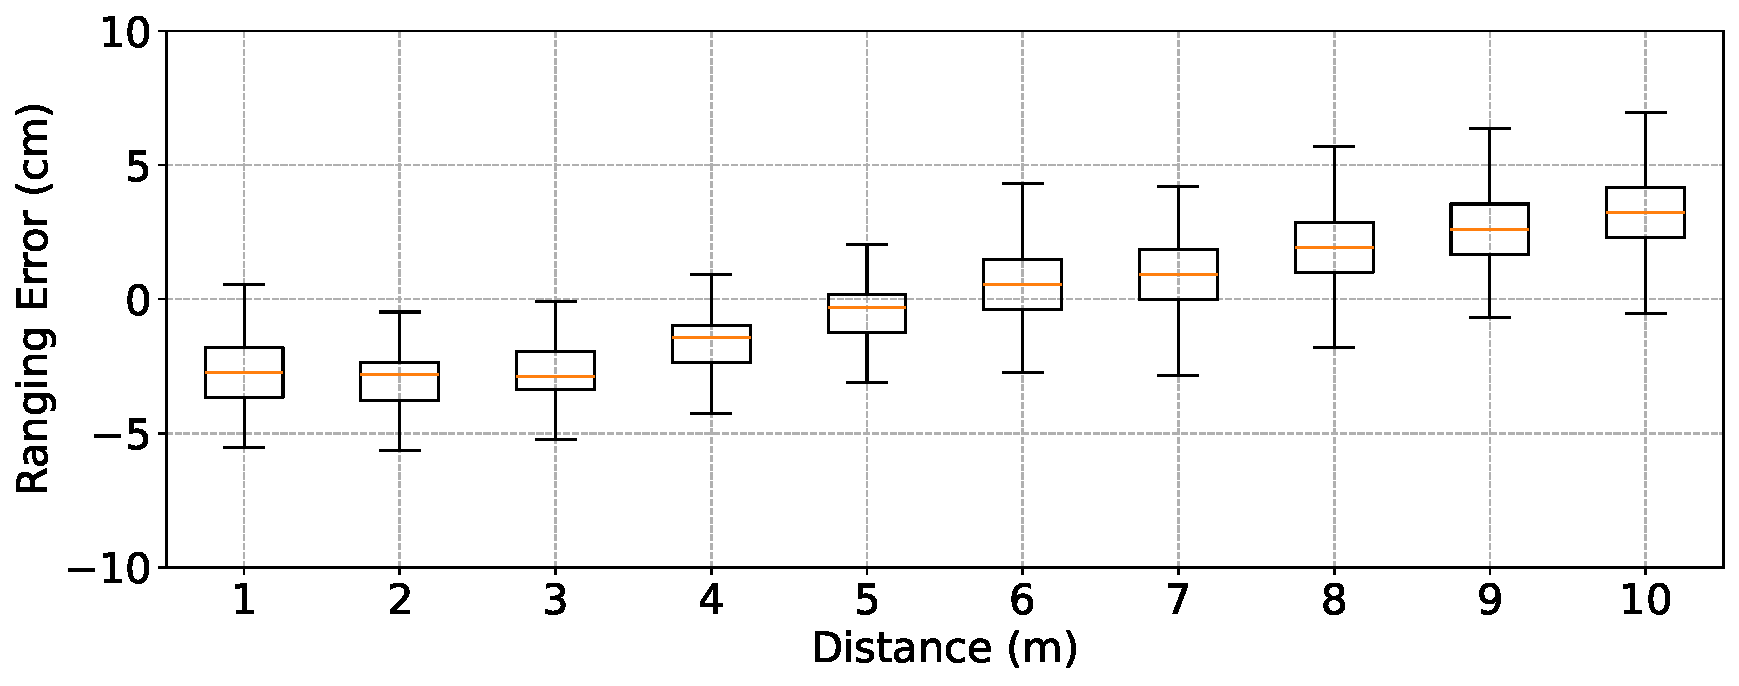
\includegraphics[width=0.8\textwidth]{Figures/experiments_and_results/ranging_accuracy_box.pdf}
    \caption[Distribution of ranging errors.]{Distribution of ranging errors across distances from 1 to 10 meters. Each box represents the interquartile range (IQR), with the horizontal line inside the box indicating the median. Whiskers extend to the data range within 1.5 IQR from the first and third quartiles.}
    \label{fig:ranging_accuracy}
\end{figure}

We evaluate the performance of the proposed ranging system in terms of key operational metrics, namely: (i) ranging accuracy and precision, (ii) ranging frequency, and (iii) quality of TDMA-based synchronization for multi-anchor operation. 

A single anchor and a fixed tag were used to collect ranging measurements at distances from 1 to 10 meters to assess the accuracy of the ranging system. At each location, \SI{\approx 1000}{} range estimates were recorded under LoS conditions. The resulting errors between measured and ground-truth distances are summarized in \autoref{fig:ranging_accuracy}. As expected, a slight systematic bias is observed: distances are underestimated at short range and overestimated at long range. This behavior is attributed to the threshold-based ToF estimation algorithm, discussed in \autoref{lde}, wherein signals with higher amplitude exhibit steeper rising edges and thus cross the detection threshold earlier than weaker signals with slower rise times.  Despite this, the absolute median error remains within \SI{\pm 5}{\centi\metre} bounds across all distances, with the overall dispersion of \SI{\approx 3}{\centi\metre}, indicating high precision.

\begin{figure}[tbh]
    \centering
    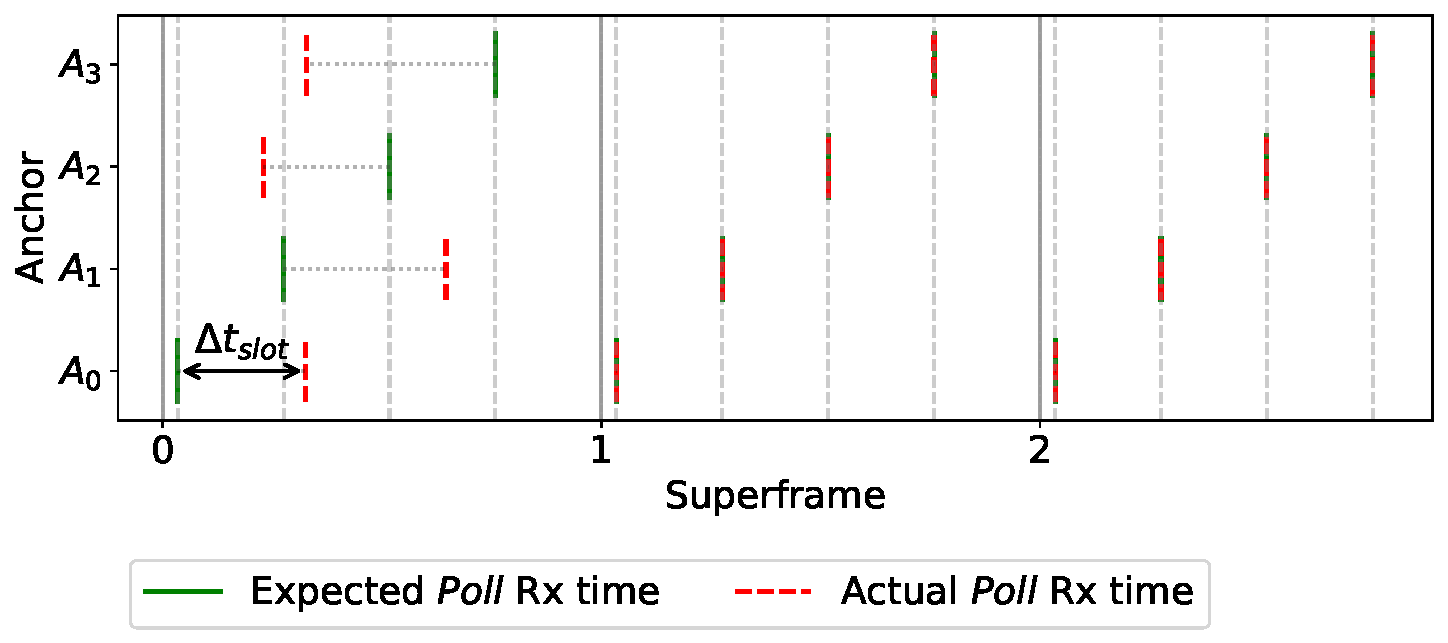
\includegraphics[width=0.8\textwidth]{Figures/experiments_and_results/sync_visualize.pdf}
    \caption[Slot synchronization timeline for a four-anchor deployment.]{Slot synchronization timeline for a four-anchor deployment. Green lines indicate the expected reception times of \textit{Poll} messages at the tag, while red dashed lines denote the actual reception times.}
    \label{fig:sync}
\end{figure}

To assess the quality of inter-device synchronization (refer to \autoref{ranging_system} for details), the timing alignment of received \textit{Poll} messages was evaluated over consecutive superframes when four anchors are active. As stated before, the observed offset, $\Delta t_{\text{slot}}$, is continuously estimated at the tag and relayed back to the anchor, which then adjusts its future slot scheduling. \autoref{fig:sync} visualizes this process. Initially, noticeable misalignments between expected and actual message arrival times are observed. However, convergence is achieved within two superframes. After correction, the residual timing jitter remains as low as approximately \SI{1}{\micro\second}.

In the current configuration, each slot was assigned a duration of \SI{3700}{\micro\second}, with a guard interval of \SI{500}{\micro\second} added at the beginning of each superframe to accommodate wake-up uncertainty and prevent overlap. This scheduling yields an effective measurement frequency of approximately \SI{67}{\hertz} per anchor, resulting in a combined rate of \SI{270}{\hertz} for the four-anchor setup used in the experiments.

\section{Dataset analysis}

\begin{figure}[tbh]
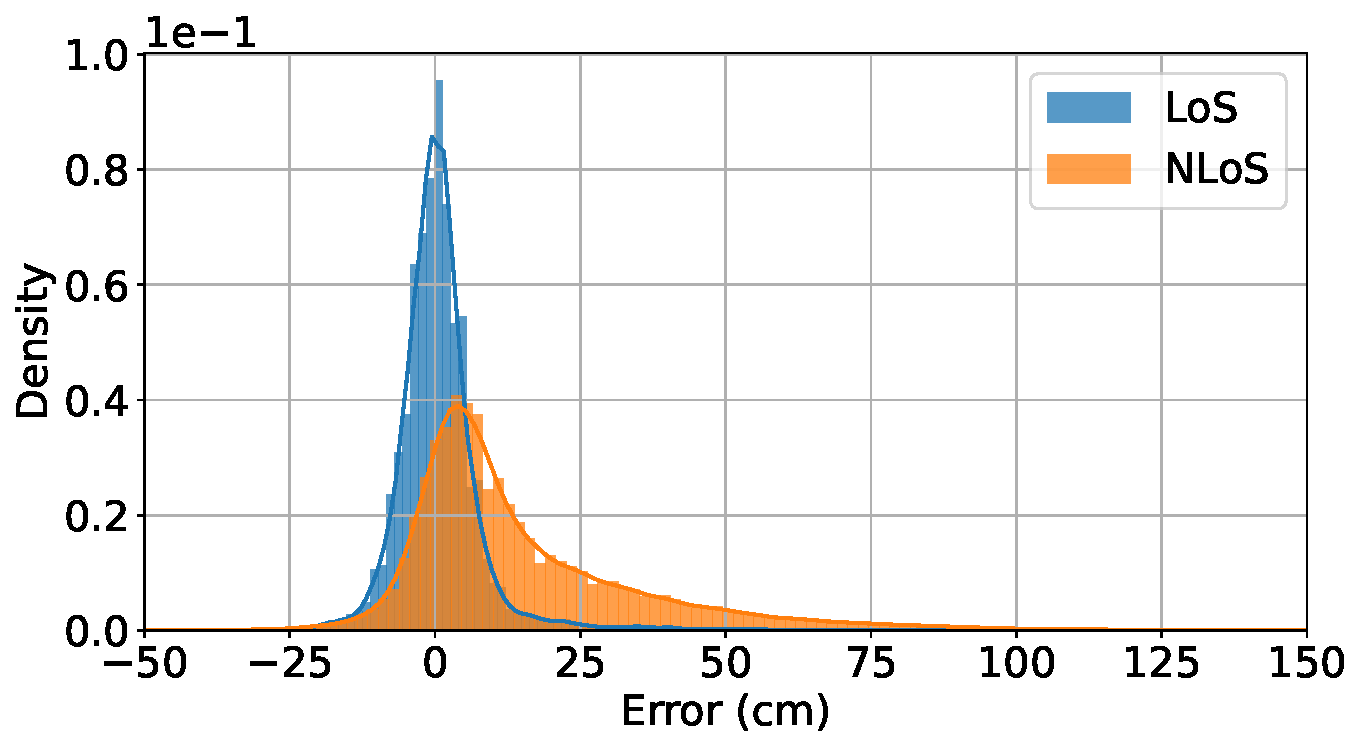
\includegraphics[width=0.7\textwidth]{Figures/experiments_and_results/dataset_error_distribution.pdf}
\centering
\caption[Empirical distribution of ranging errors in \textit{RangeCIR} dataset.]{Empirical distribution of ranging errors in \textit{RangeCIR} dataset under LoS and NLoS conditions.}
\label{fig:err_dist}
\end{figure}

The \textit{RangeCIR} dataset presented in \autoref{data_collection} consists of 990\,147 samples, spanning ranges between 1 and 7.5 meters. The experimental procedure ensured comprehensive coverage of both LoS and realistic NLoS scenarios, simulated with human obstruction, yielding a balanced distribution of approximately \SI{55}{\percent} LoS and \SI{45}{\percent} NLoS samples. \autoref{fig:err_dist} illustrates the empirical distribution of ranging errors under LoS and NLoS conditions. The LoS errors exhibits a sharp unimodal peak centered around zero, indicative of stable and low-variance performance under unobstructed conditions. Conversely, the NLoS error distribution is positively skewed with increased dispersion, closely resembling a log-normal distribution for the positive-valued portion of the data, reflecting multipath-induced bias due to human obstructions.

\begin{table}[tbh] 
\centering 
\caption[Summary of ranging error statistics in the proposed dataset.]{Summary of ranging error statistics in the proposed dataset. $\mu$: mean error, $\sigma$: standard deviation, MAE: mean absolute error. All values in centimeters.} \label{tab:error_stats} 
\begin{tabular}{lccc} 
\toprule 
\textbf{Condition} & $\mathbf{\mu}$ & $\mathbf{\sigma}$ & \text{MAE} \\ 
\midrule 
LoS & 3.6 & 7.7 & 5.6 \\
NLoS & 18.4 & 21 & 19.4 \\
Overall & 10.3 & 16.9 & 11.8 \\ 
\bottomrule 
\end{tabular} 
\end{table}

\autoref{tab:error_stats} summarizes the statistical properties of these errors. Across the entire dataset, the ranging error varies from \SI{-50}{\centi\metre} to \SI{219}{\centi\metre}, yielding a mean of \SI{10.3}{\centi\metre}, a standard deviation of \SI{16.9}{\centi\metre}, and a mean absolute error (MAE) of \SI{11.8}{\centi\metre}. For isolated LoS measurements, we report a mean of \SI{3.6}{\centi\metre}, and a standard deviation of \SI{7.7}{\centi\metre}. In contrast, the data labeled as NLoS has significantly higher bias and dispersion (mean \SI{18.4}{\centi\metre}, standard deviation \SI{21}{\centi\metre}), resulting in an MAE of \SI{5.6}{\centi\metre} for LoS and \SI{19.4}{\centi\metre} for NLoS measurements.


\section{A-REMNet results}

\subsection{Training and inference setup}
The proposed A-REMNet model was implemented in PyTorch Python framework and trained on a filtered subset of the collected dataset (\autoref{data_collection}). To prevent overfitting to LoS conditions, which tend to exhibit low error variability, the dataset was rebalanced to contain \SI{70}{\percent} NLoS samples. The resulting dataset comprised 640\,715 samples, partitioned into training, validation, and test subsets (70/20/10), with measurement samples randomly distributed across splits.

CIR samples were extracted as complex-valued tensors of shape $K \times 2$, where $K = 133$ corresponds to a fixed window around the first path index, including 5 samples before and 127 after. This window was empirically selected for optimal performance. Each CIR sample was paired with a scalar ground truth error label.

Model hyperparameters were tuned using Bayesian optimization on the validation set. The final configuration included $F = 64$ low-level feature channels and $N = 5$ RRMs. To balance complexity and ensure sufficient temporal resolution for effective operation, a self-attention unit with $h = 4$ heads was included in the first two RRMs only. The reduction ratio of the SE block is set to $r = 8$. The kernel sizes of the convolutional layers are retained from the original study: 7 for the initial convolution, 3 for the residual units and the first branch of the reduction block, and 1 for the second branch. This configuration results in approximately 200K trainable parameters.

To assess computational feasibility, empirical complexity analysis was conducted using Meta's \texttt{fvcore} profiling tool. The model was found to require approximately 11.7 million floating-point operations (FLOPs) per forward pass. Inference latency was measured on an NVIDIA GeForce RTX 2080Ti GPU, yielding a mean runtime of \SI{2.9}{\milli\second} per sample with a standard deviation of \SI{0.05}{\milli\second}.

Training was performed with a batch size of 256 for up to 100 epochs using the Adam optimizer with a learning rate of $10^{-3}$. To prevent overfitting, early stopping with a patience of 5 epochs was applied based on validation loss monitoring. To handle the heavy-tailed error distribution of the dataset, particularly under NLoS conditions, the model was trained using the Huber loss, which balances sensitivity to small errors with robustness to outliers:

\begin{equation} 
\mathcal{L}_{\delta}(e) = 
\begin{cases} 
\frac{1}{2}e^2, & \text{if}\ |e| \leq \delta,\\
\delta \left(|e| - \frac{1}{2}\delta\right), & \text{otherwise}, 
\end{cases} 
\end{equation}
where $e$ denotes the prediction error and $\delta = 1.0$ defines the transition point between quadratic and linear regimes. The training process is completed in approximately 20 minutes.

\subsection{Quantitative results}

\begin{table}[tbh] 
\centering 
\caption[Error statistics before and after mitigation.]{Error statistics on the test set before and after mitigation. All values in centimeters. Refer to \autoref{tab:error_stats} for notation definitions.} 
\label{tab:test_results} 
\begin{tabular}{lccc|ccc|c} 
\toprule 
\multirow{2}{*}{\textbf{Condition}} 
& \multicolumn{3}{c|}{\textit{Before mitigation}} 
& \multicolumn{3}{c|}{\textit{After mitigation}} 
& \textit{Improvement} \\
& $\mu$ & $\sigma$ & MAE & $\mu$ & $\sigma$ & MAE & $\Delta$MAE \\
\midrule 
LoS     & 3.7  & 7.8  & 5.6  & -0.2 & 3.8 & 2.2 & \textbf{61 \%} \\
NLoS    & 18.3 & 21.1 & 19.4 & 0.8  & 9.8 & 5.5 & \textbf{71 \%} \\
Overall & 14.0 & 19.4 & 15.3 & 0.5  & 8.5 & 4.5 & \textbf{70 \%} \\
\bottomrule 
\end{tabular} 
\end{table}

\autoref{tab:test_results} reports error statistics on the test set. The model reduces the overall MAE from \SI{15.3}{\centi\metre} to \SI{4.5}{\centi\metre}, corresponding to a relative improvement of \SI{70}{\percent}. Notably, even in LoS conditions, where errors are typically low, the model still reduces the MAE from \SI{5.6}{\centi\metre} to \SI{2.2}{\centi\metre}, amounting to a \SI{61}{\percent} relative improvement. This suggests that the network learned to model subtle, deterministic biases present in LoS CIRs, which we believe likely arise from antenna orientation characteristics. In NLoS scenarios, where the error variance is higher, the MAE decreases from \SI{19.4}{\centi\metre} to \SI{5.5}{\centi\metre}, yielding a relative improvement of \SI{71}{\percent}. In all cases, the standard deviation of residuals is also significantly lower, indicating improved consistency across estimates.

\begin{figure}[tbh] 
\centering 
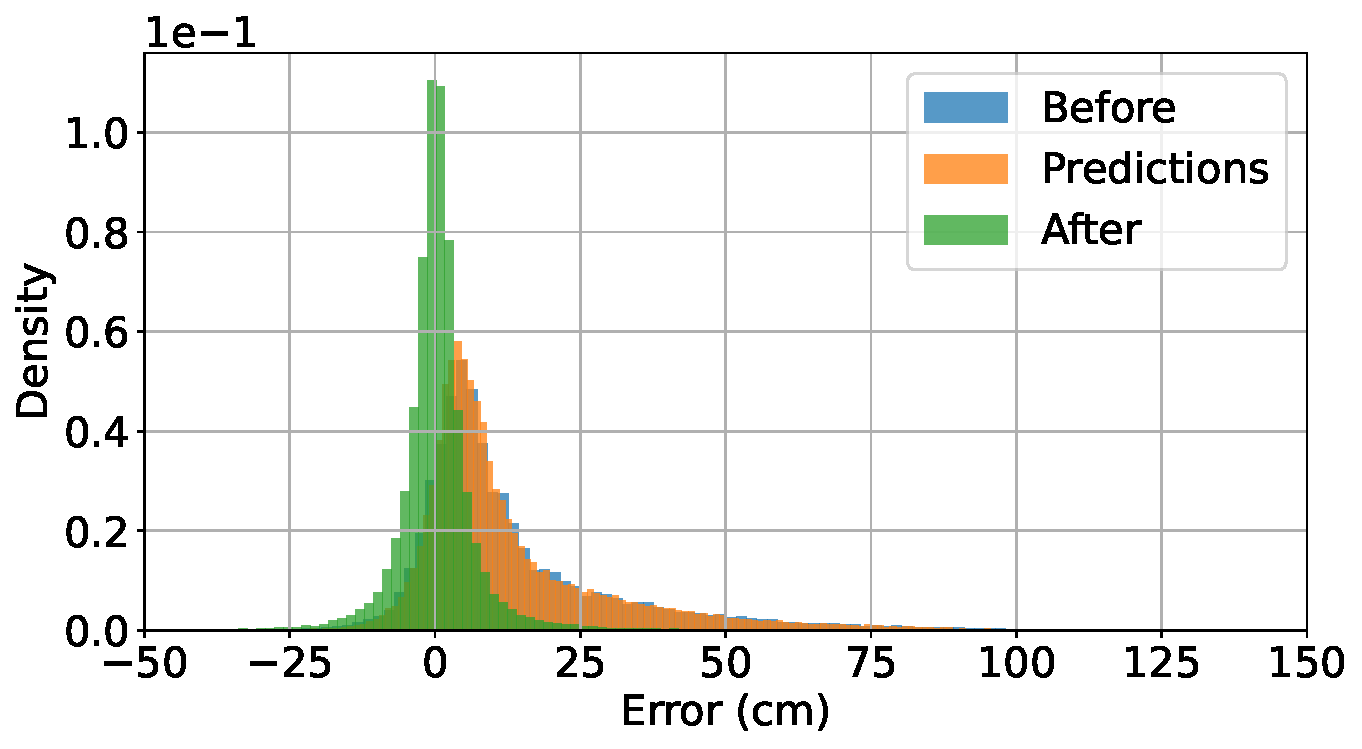
\includegraphics[width=0.7\textwidth]{Figures/experiments_and_results/model_error_distribution.pdf} 
\caption[Distributions of errors before and after mitigation.]{Distributions of errors before and after mitigation, along with model-predicted errors on the test set.} \label{fig:error_distribution} 
\end{figure}

\autoref{fig:error_distribution} shows the empirical distributions of observed, predicted, and residual errors. Notably, the residual error distribution is approximately Gaussian, centered near zero ($\mu = 0.5$). This is a desirable property in localization pipelines, where zero-mean noise aligns with common assumptions in Kalman filters (\autoref{kalman_theory}).

\subsubsection{Ablation study}
To assess the contribution of the proposed attention mechanism, we conducted an ablation study by removing the attention unit from each RRM, while preserving all other architectural components, hyperparameters, training configuration, and dataset splits. The resulting baseline model is structurally identical to A-REMNet, apart from the absence of the attention unit, and comprises 151\,337 trainable parameters (compared to 200\,425 in the full model).

\begin{table}[tbh]
\centering
\caption[Error statistics with and without the attention mechanism.]{Comparison of test set error statistics with and without the attention mechanism. All values in centimeters. Refer to \autoref{tab:error_stats} for notation definitions.}
\label{tab:ablation_results}
\begin{tabular}{lccc|ccc|c}
\toprule
\multirow{2}{*}{\textbf{Condition}} &
\multicolumn{3}{c|}{\textit{No Attention}} &
\multicolumn{3}{c|}{\textit{With Attention}} &
\textit{Improvement} \\
& $\mu$ & $\sigma$ & MAE & $\mu$ & $\sigma$ & MAE & $\Delta$MAE \\
\midrule
LoS     & -0.7 & 4.1  & 2.4 & -0.2 & 3.8 & 2.2 & \textbf{8 \%} \\
NLoS    & 1.0  & 11.0 & 6.3 & 0.8  & 9.8 & 5.5 & \textbf{13 \%} \\
Overall & 0.5  & 9.5  & 5.1 & 0.5  & 8.5 & 4.5 & \textbf{12 \%} \\
\bottomrule
\end{tabular}
\end{table}

\autoref{tab:ablation_results} summarizes the results for both variants. Removal of the attention unit results in a degradation of error mitigation performance across all conditions. The overall MAE increases from \SI{4.5}{\centi\metre} to \SI{5.1}{\centi\metre}, corresponding to a relative improvement of \SI{12}{\percent} in favor of the attention-based model. This is accompanied by a higher standard deviation of residuals (\SI{9.5}{\centi\metre} vs.\ \SI{8.5}{\centi\metre}). The effect is most pronounced under NLoS conditions, where the residual MAE increases by \SI{13}{\percent}, from \SI{5.5}{\centi\metre} to \SI{6.3}{\centi\metre}. Interestingly, however, a performance gap of \SI{8}{\percent} is also observed under LoS conditions, where MAE increases from \SI{2.2}{\centi\metre} to \SI{2.4}{\centi\metre}, indicating that the attention unit is beneficial even in lower-error conditions.

These results suggest that the self-attention mechanism contributes substantially to the model's ability to extract temporal dependencies in the CIR sequence and suppress likely complex error patterns, particularly under NLoS conditions.


\section{Experimental results}

To evaluate the end-to-end performance of the proposed IPS pipeline, which integrates A-REMNet-based error mitigation with EKF-based localization, we conducted a series of trajectory reconstruction experiments under varying conditions. Three scenarios were tested: (i) no obstacles (clear LoS), (ii) obstructed paths in a known (seen before) environment used during dataset collection (see \autoref{data_collection}), and (iii) obstructed paths in a previously unseen environment. Each scenario included two movement patterns: a rectangular loop and an hourglass-shaped trajectory.

\subsection{Experimental setup}

\begin{figure}[tbh]
    \centering
    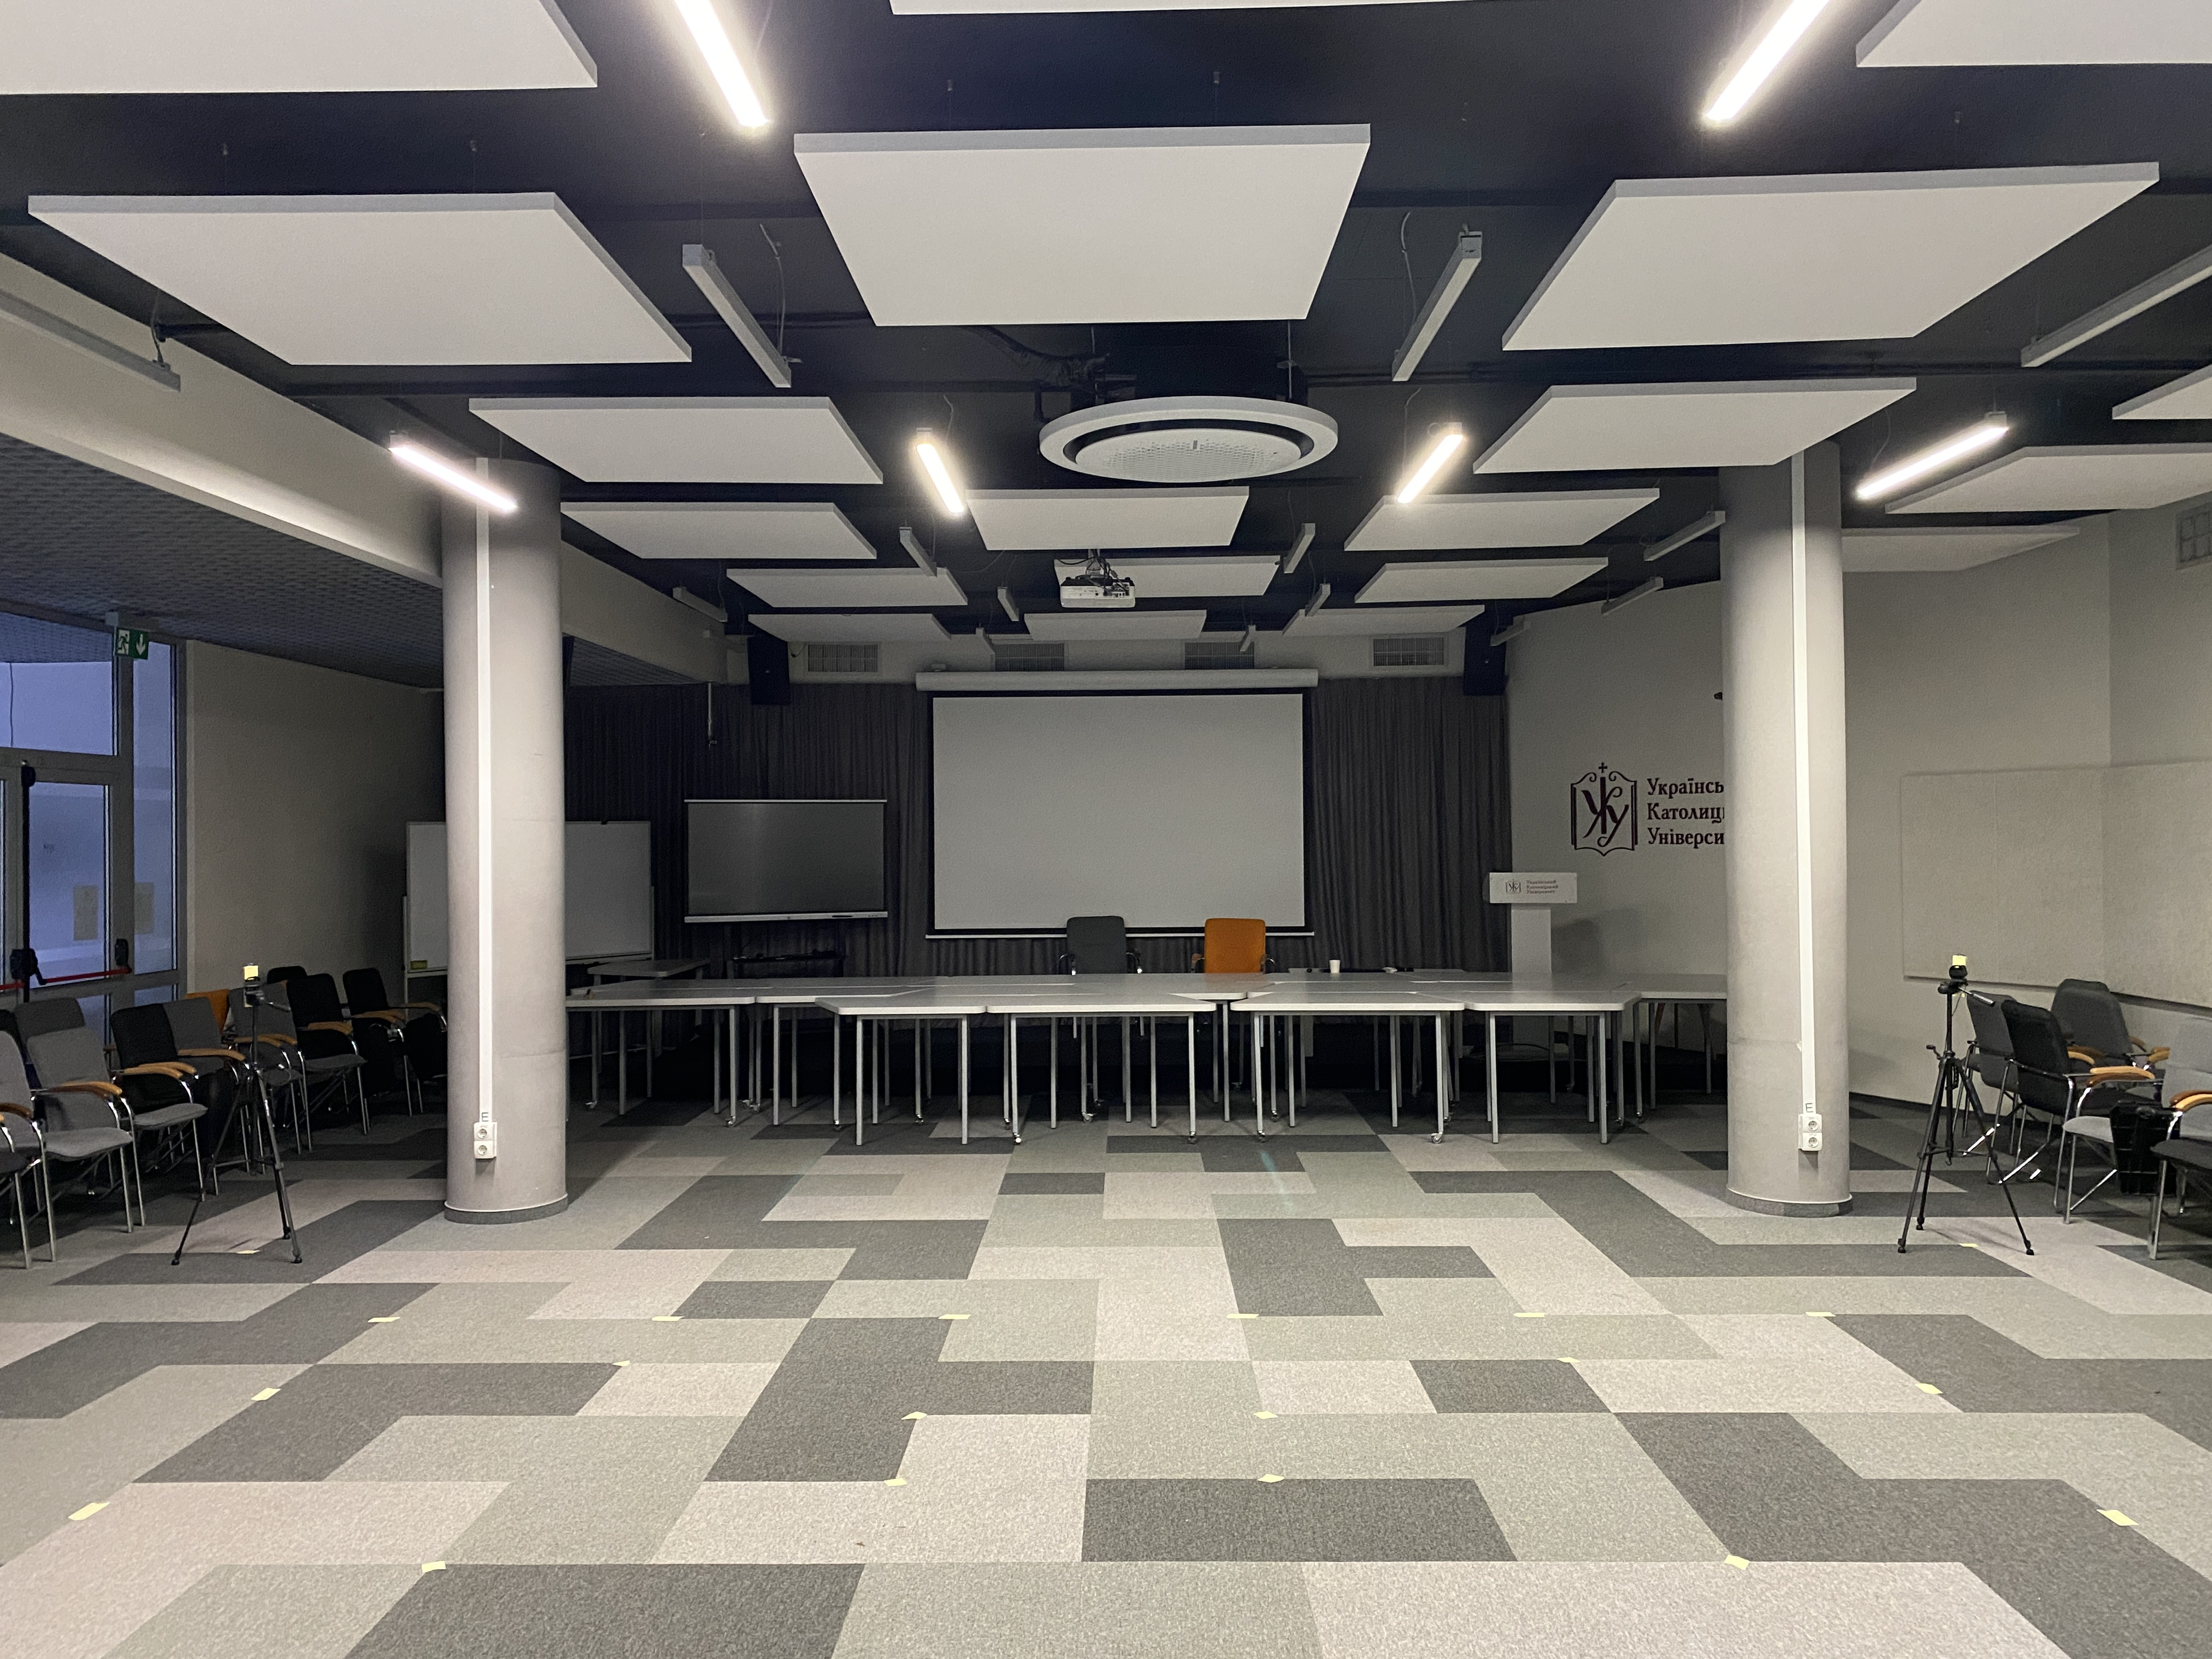
\includegraphics[width=0.7\textwidth]{Figures/experiments_and_results/evaluation_env.png}
    \caption[Unseen evaluation environment.]{Unseen evaluation environment. The space differs structurally, geometrically, and visually from the training environment.}
    \label{fig:unseen_environment}
\end{figure}

All experiments were carried out in indoor environments, with four UWB anchors mounted on tripods around the corners of the trajectory frame. The tag was handheld and moved by a human subject at a consistent walking speed (\SI[per-mode=symbol]{\approx 3}{\kilo\metre\per\hour}) along pre-marked paths. For the obstructed configurations, four individuals continuously moved along the LoS paths between the transceivers, thereby maintaining persistent blockage of the direct signal path. We want to elaborate, that the unseen environment, depicted in \autoref{fig:unseen_environment}, was not used during training, and serving as a testbed for evaluating the generalization capability of the error mitigation model.

Ground truth positions were derived from the known trajectory geometry, with synchronization timing recovered from ceiling-mounted camera video recordings. Due to inherent human movement variance, the subject's adherence to the marked trajectory was accurate to within approximately \SI{10}{\centi\meter}. Given the slight remaining mismatch in timing between the human-executed path and the inferred ground-truth position estimates, particularly around corners, the Dynamic Time Warping (DTW) algorithm~\cite{dtw}, implemented via the \texttt{fastdtw} Python library, was used to temporally align the estimated and reference trajectories by computing an optimal index-wise correspondence between them under continuity and monotonicity constraints. The resulting warping path was used to derive pointwise errors and enabled robust MAE evaluation, despite natural speed variations.

% Given the slight remaining mismatch in timing between the human-executed path and the inferred ground-truth position estimates, especially around trajectory corners, the DTW algorithm~\cite{dtw} was applied to align the estimated and ground-truth trajectories. 

% Let $\mathbf{X} = \{ \mathbf{x}_1, \dots, \mathbf{x}_N \}$ and $\mathbf{Y} = \{ \mathbf{y}_1, \dots, \mathbf{y}_M \}$ denote the estimated and ground truth trajectories, respectively. DTW computes an optimal alignment path $\mathcal{W}$ of length $K$, defined as a sequence of index pairs $(i_k, j_k) \mid i_k \in [1, N],\ j_k \in [1, M]$, by minimizing the total pointwise Euclidean distance under continuity and monotonicity constraints:
% \begin{equation}
% \mathcal{W}^* = \arg \min_{\mathcal{W}} \sum_{k=1}^{K} \| \mathbf{x}_{i_k} - \mathbf{y}_{j_k} \|_2.
% \end{equation}
% Each pair $(i_k, j_k)$ indicates that the $i_k$-th point of the estimated trajectory is matched with the $j_k$-th point of the ground truth trajectory. The resulting path was used to derive pointwise absolute errors, enabling robust computation of the MAE even in the presence of natural speed variations.


Under conditions without obstacles, we conducted only three repetitions of each experiment due to low variance in the resulting measurements. For setups with obstacles, each experiment was repeated five to seven times to ensure statistical significance of the results. For each experiment, the estimated range measurements were processed through the proposed Kalman filter, applied in two variants: with and without prior error correction using A-REMNet model. The filter parameters were tuned using the normalized innovation squared (NIS) and normalized estimation error squared (NEES) metrics to ensure the statistical consistency of the filter. Specifically, we select noise covariances $\mathbf{Q}, \mathbf{R}$ such that \SI{\approx 95}{\percent} of the NIS and NEES values remained within the theoretical confidence bounds ($\chi^2$ distribution) for their respective degrees of freedom. In our experiments, we set $\mathbf{Q} = 10^{-4} \cdot \mathbf{I}_4$, and $\mathbf{R} = 0.3$.

\subsection{Performance evaluation}
\subsubsection{Quantitative results}

\begin{figure}[tbh]
    \centering
    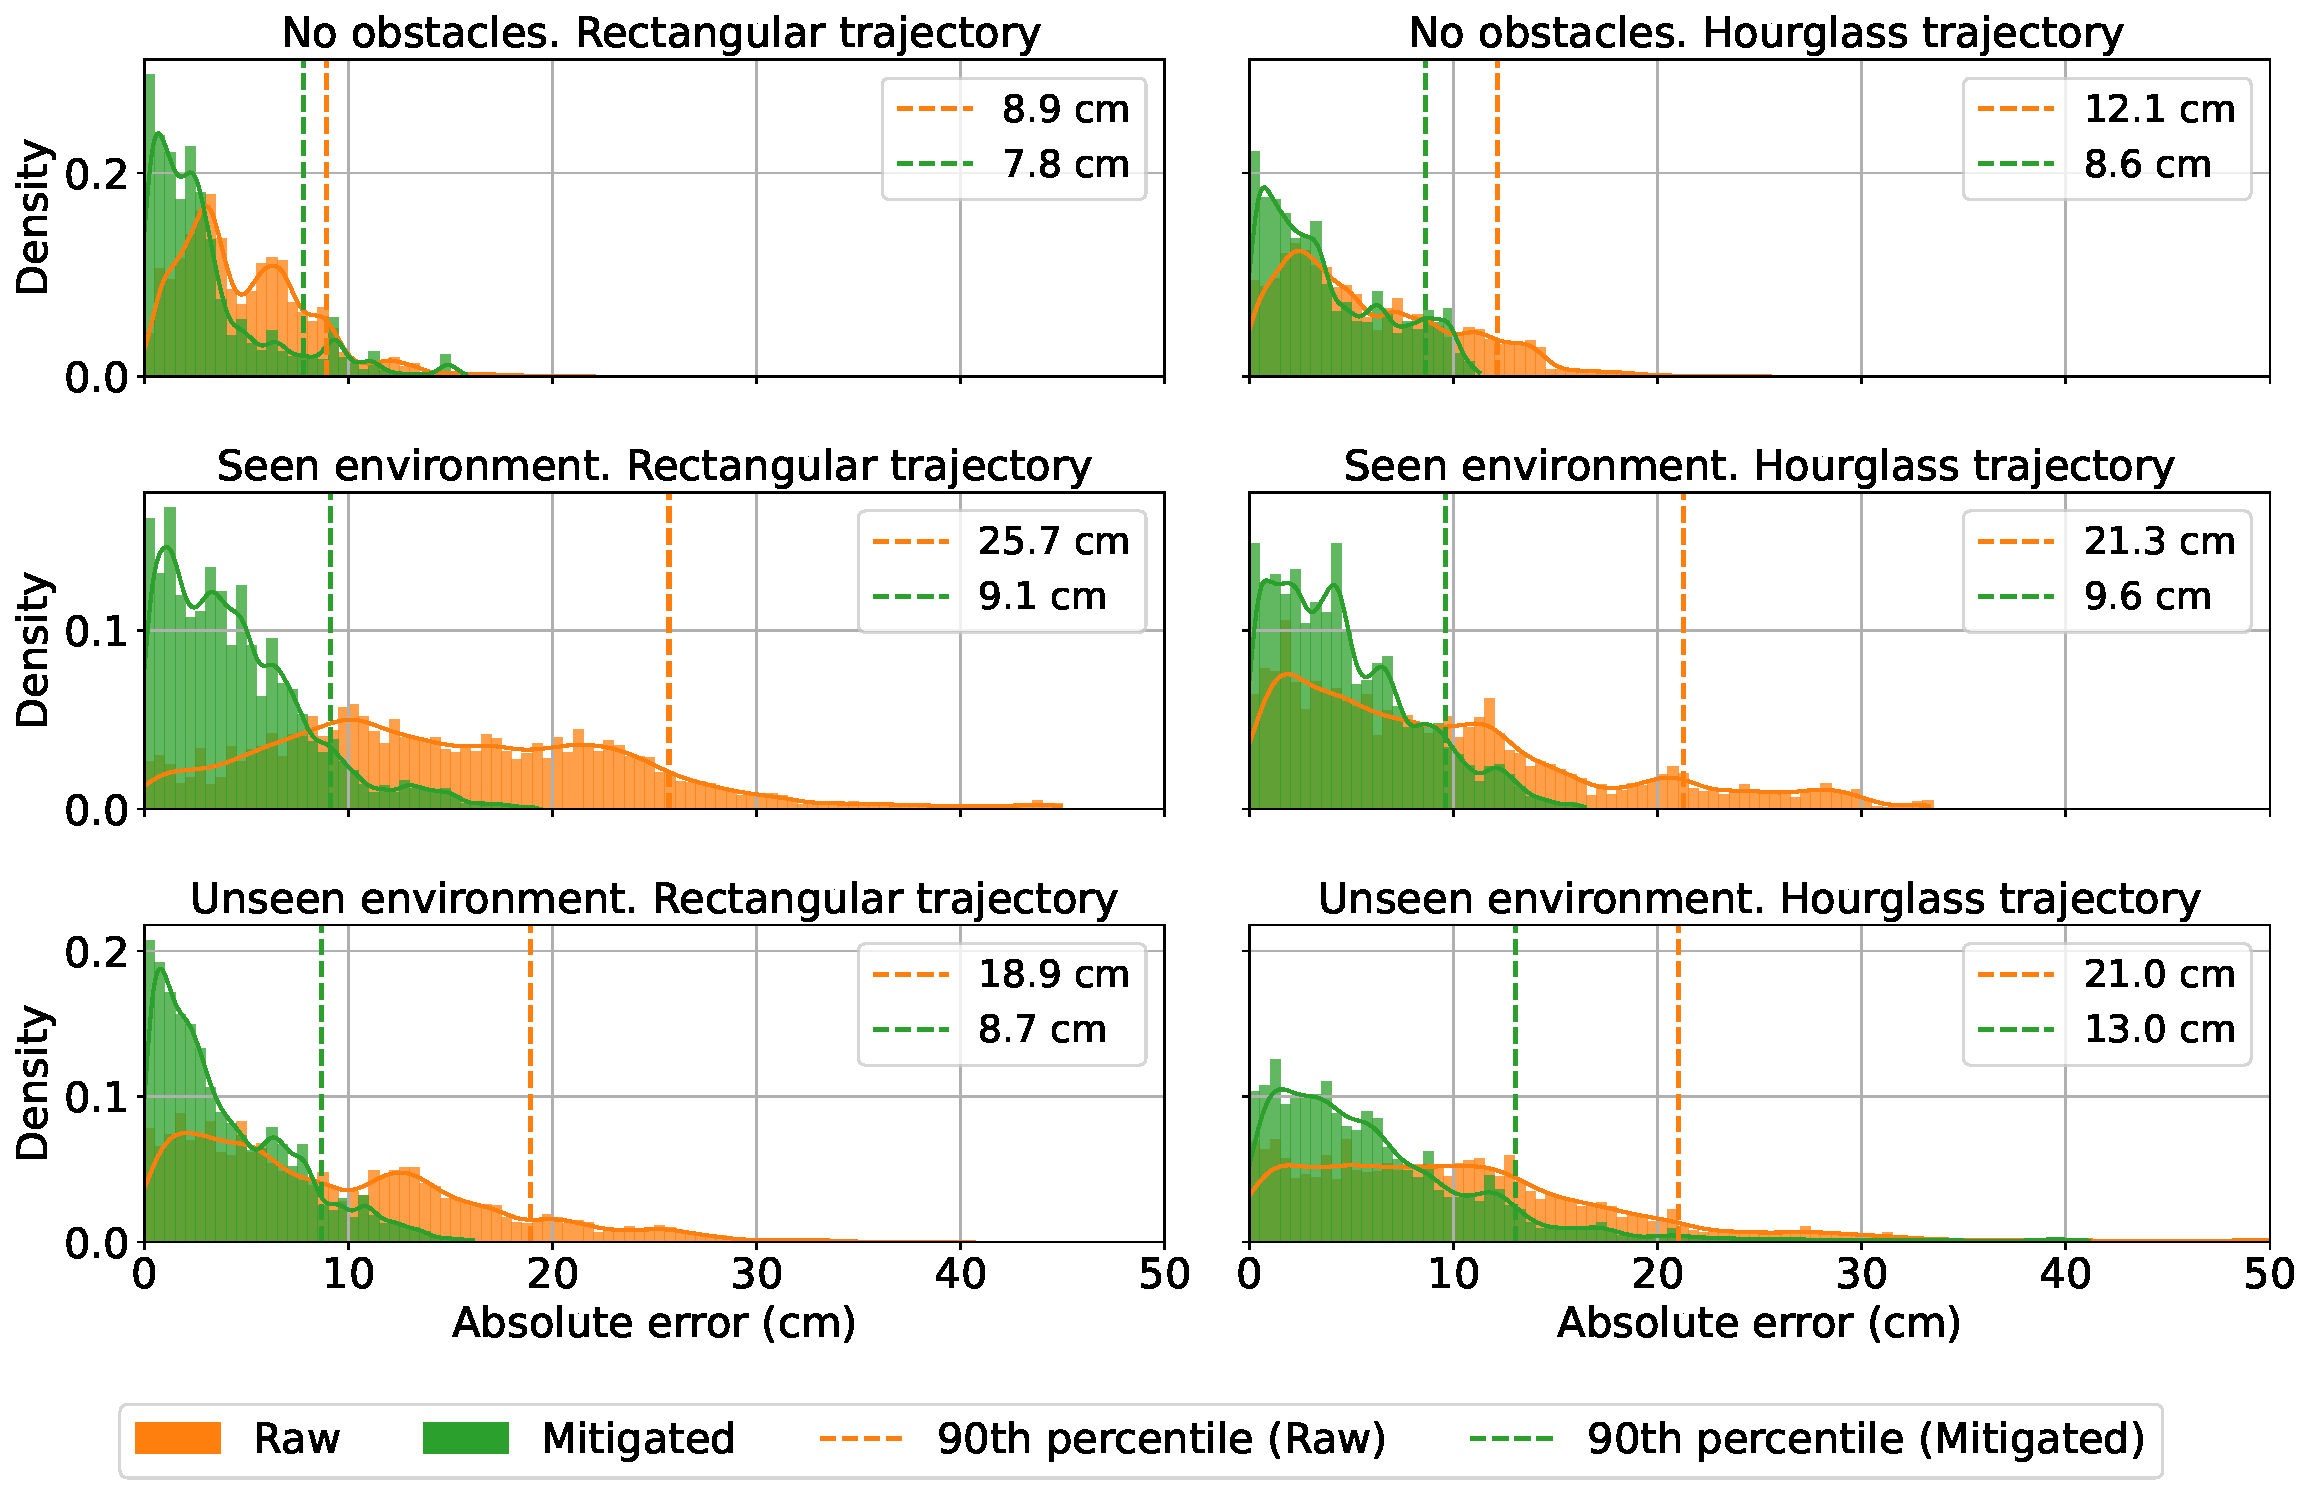
\includegraphics[width=\textwidth]{Figures/experiments_and_results/dtw_errors.pdf}
    \caption[Empirical distributions of localization errors before and after mitigation.]{Empirical distributions of pointwise localization errors before (raw) and after mitigation (mitigated), computed across all experimental repetitions.}
    \label{fig:dtw_errors}
\end{figure}

\autoref{fig:dtw_errors} presents the empirical distributions of pointwise localization errors across all experimental conditions, stratified by environment and trajectory. These are complemented by the corresponding MAE statistics shown in \autoref{fig:dtw_errors_mae_box}, and detailed in \autoref{tab:mae-improvement}, which reports the median MAE before and after error mitigation, along with relative improvements.

Across all evaluated conditions, the error mitigation module consistently yields significant performance gains. As seen in \autoref{fig:dtw_errors}, the application of the proposed model results in a pronounced leftward shift in the error density, indicating a general reduction in estimation errors. Additionally, a consistent decrease in residual error dispersion and MAE is observed, as summarized in \autoref{fig:dtw_errors_mae_box}.

\begin{table}[tbh]
\centering
\caption[Median error and relative improvement for each setup.]{Median MAE and relative improvement for each setup. All values are in centimeters. The $\pm$ denotes standard deviation.}
\label{tab:mae-improvement}
\begin{tabular}{llccc}
\toprule
\textbf{Setup} & \textbf{Trajectory} & \multicolumn{2}{c}{\textbf{MAE}} & \textbf{Improvement} \\
\cmidrule(lr){3-4}
 & & \textit{Raw} & \textit{Mitigated} & \\
\midrule
\multirow{2}{*}{No obstacles} 
  & Rectangular &  5.0 $\pm$ 0.3 & 3.1 $\pm$ 0.3 & \textbf{38} $\pm$ 1 \% \\
  & Hourglass   &  5.8 $\pm$ 0.1 & 3.8 $\pm$ 0.2 & \textbf{33} $\pm$ 3 \% \\
\midrule
\multirow{2}{*}{Seen environment} 
  & Rectangular & 15.9 $\pm$ 0.9 & 4.4 $\pm$ 0.1 & \textbf{70} $\pm$ 4 \% \\
  & Hourglass   &  8.6 $\pm$ 0.6 & 4.5 $\pm$ 0.4 & \textbf{47} $\pm$ 6 \% \\
\midrule
\multirow{2}{*}{Unseen environment} 
  & Rectangular &  9.3 $\pm$ 1.7 & 3.8 $\pm$ 0.5 & \textbf{58} $\pm$ 3 \% \\
  & Hourglass   & 11.9 $\pm$ 1.2 & 7.0 $\pm$ 1.2 & \textbf{41} $\pm$ 3 \% \\
\bottomrule
\end{tabular}
\end{table}

\begin{figure}[tbh]
    \centering
    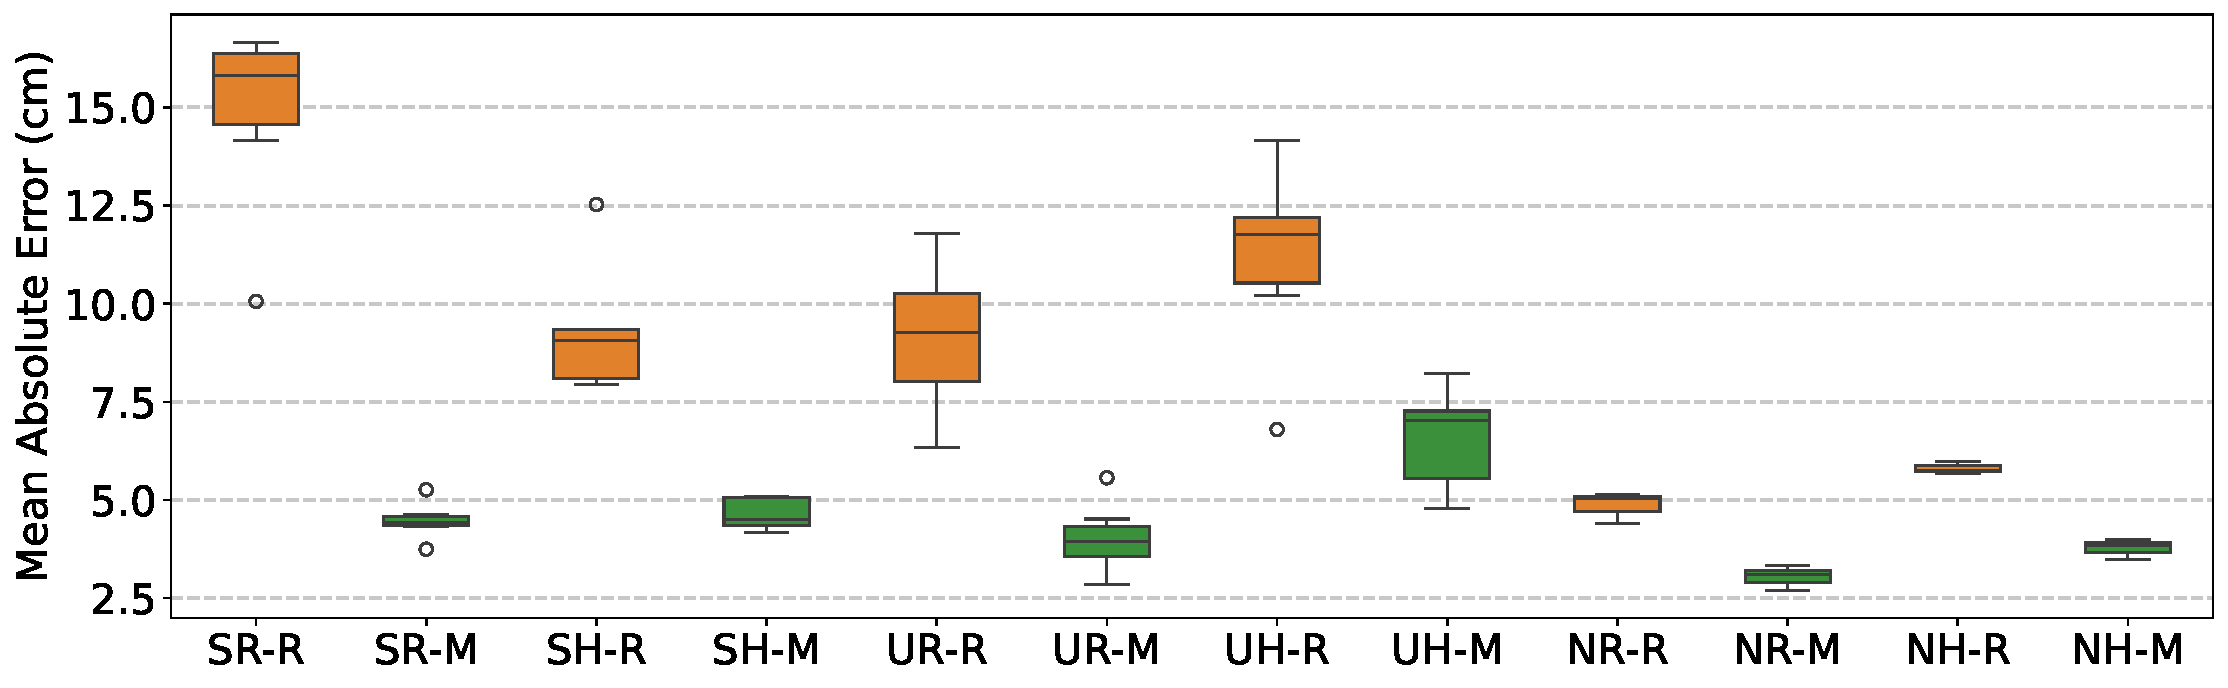
\includegraphics[width=\textwidth]{Figures/experiments_and_results/dtw_errors_mae_box.pdf}
    \caption[Statistics of mean absolute error across all evaluation setups.]{Statistics of MAE across evaluation setups. X-axis labels denote the environment (N -- no obstacles, S -- seen, U -- unseen), trajectory (R -- rectangular, H -- hourglass), and method (R -- raw (orange), M -- mitigated (green)). Individual dots indicate outliers. Refer to \autoref{fig:ranging_accuracy} for details on the interpretation of box plot elements.}
    \label{fig:dtw_errors_mae_box}
\end{figure}

In the LoS configuration, where the initial localization errors are already relatively small (median MAE ranging from 5.0 to 5.8 \si{\centi\meter}), the model achieves a relative improvement of 33-38 \si{\percent}, reducing the residual error to 3.1-3.8 \si{\centi\meter}. Notably, that these values closely approach the fundamental accuracy limits of the ranging subsystem, as established in prior evaluation. We believe, that observed correction likely reflects the model’s capacity to account for systematic errors, such as those arising from antenna radiation patterns, as earlier hypothesized.

The most substantial improvements are observed in the seen NLoS configuration. Here, the mitigation effectively suppresses heavy error tails and significantly reduces the 90th percentile error by up to \SI{16}{\centi\metre}. In particular, the rectangular trajectory exhibits a reduction in median MAE from \SI{15.9}{\centi\metre} to \SI{4.4}{\centi\metre}, corresponding to a \SI{70}{\percent} improvement. For the hourglass trajectory, the error decreases from \SI{8.6}{\centi\metre} to \SI{4.5}{\centi\metre} (\SI{47}{\percent} improvement). While the overall dispersion is also reduced, the gains are smaller than for the rectangular path. This discrepancy is likely related to the increased complexity of the hourglass-shaped trajectory, introduced by sharper turns and a higher likelihood of self-shadowing from the moving subject in this configuration.

In the unseen environment, performance degrades slightly, as expected. Nevertheless, the model continues to achieve meaningful improvements across all runs. The 90th percentile error is reduced by up to \SI{10}{\centi\metre}, and the MAE remains significantly improved. The rectangular trajectory again yields better results, with the MAE decreasing from \SI{9.3}{\centi\metre} to \SI{3.8}{\centi\metre} (\SI{58}{\percent} improvement). For the hourglass trajectory, the error is reduced from \SI{11.9}{\centi\metre} to \SI{7.0}{\centi\metre}, corresponding to a \SI{41}{\percent} improvement. Notably, for the latter configuration, we do not observe a reduction in error dispersion, suggesting that residual errors in retain greater variability. Nonetheless, the overall error remains significantly reduced, and the results indicate that the model generalizes well, achieving \SI{50}{\percent} MAE reduction on average in the unseen setting.

\subsubsection{Qualitative results}

\begin{figure}[tbh]
    \centering
    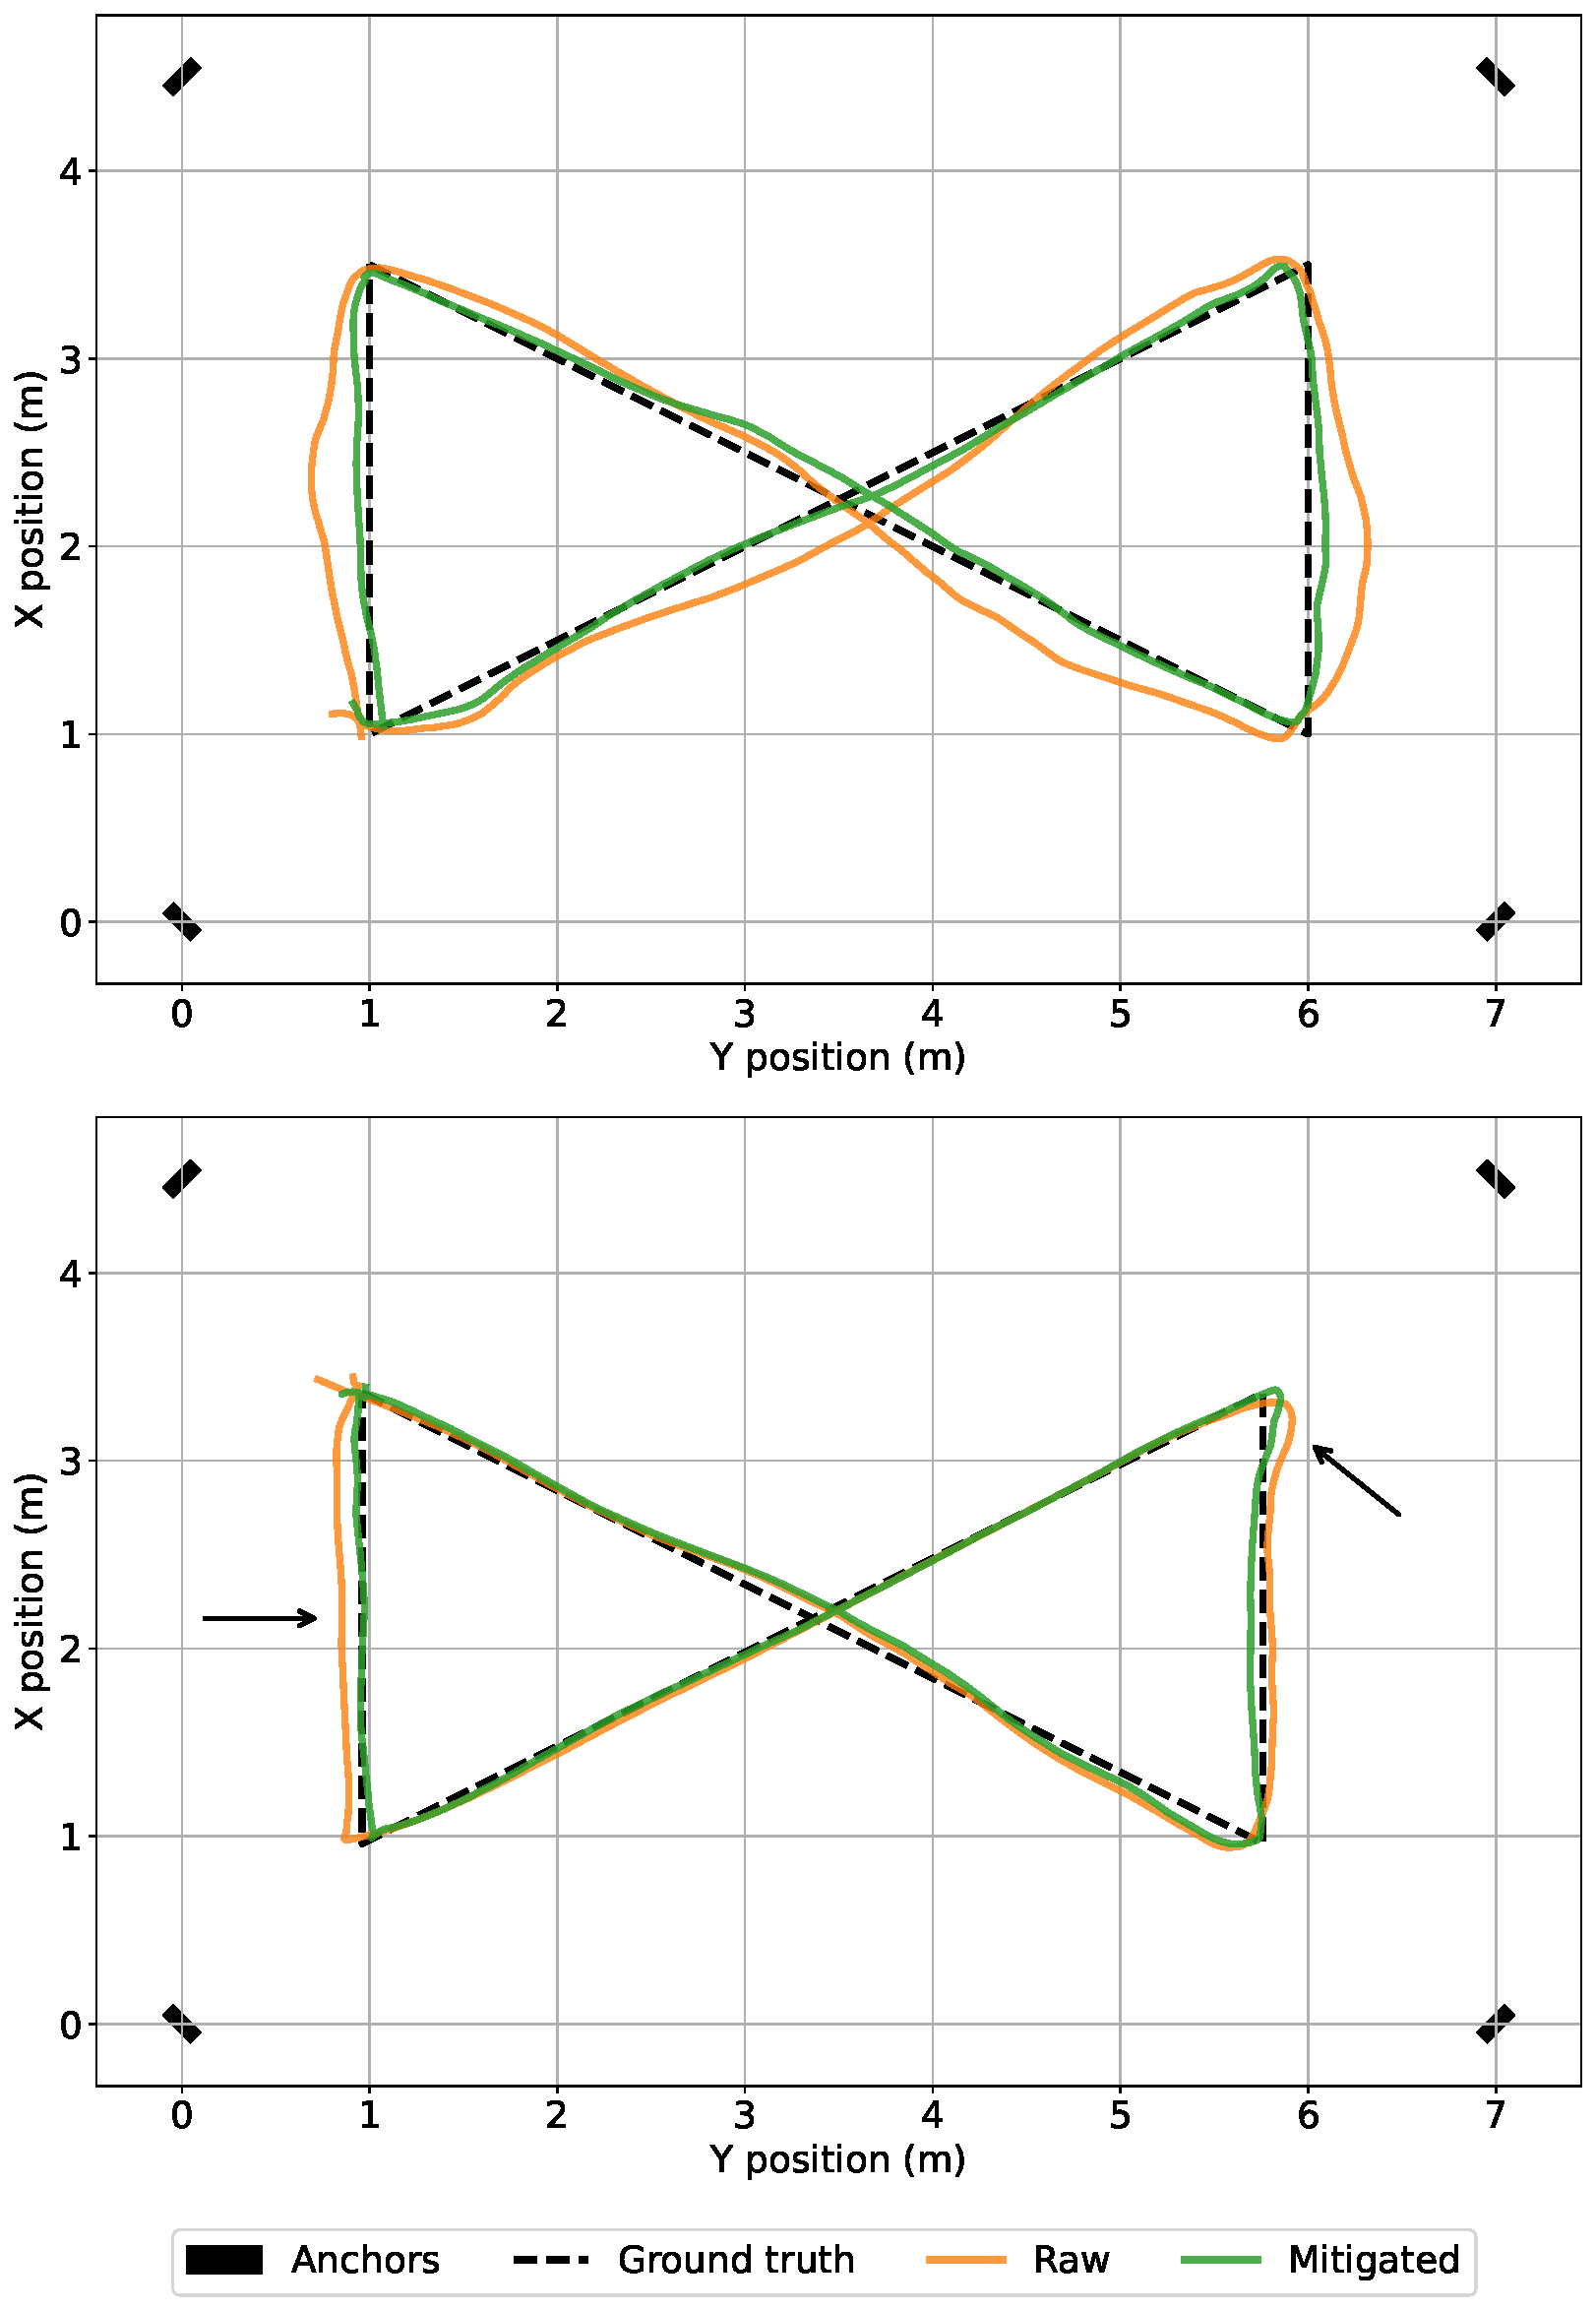
\includegraphics[width=0.85\textwidth]{Figures/experiments_and_results/hourglass_trajectory.pdf}
    \caption{Trajectory reconstruction results for the hourglass trajectory in both LoS (top) and unseen NLoS (bottom) scenarios. Arrows annotate key regions of improvement.}
    \label{fig:trajectories_hourglass}
\end{figure}

\begin{figure}[tbh]
    \centering
    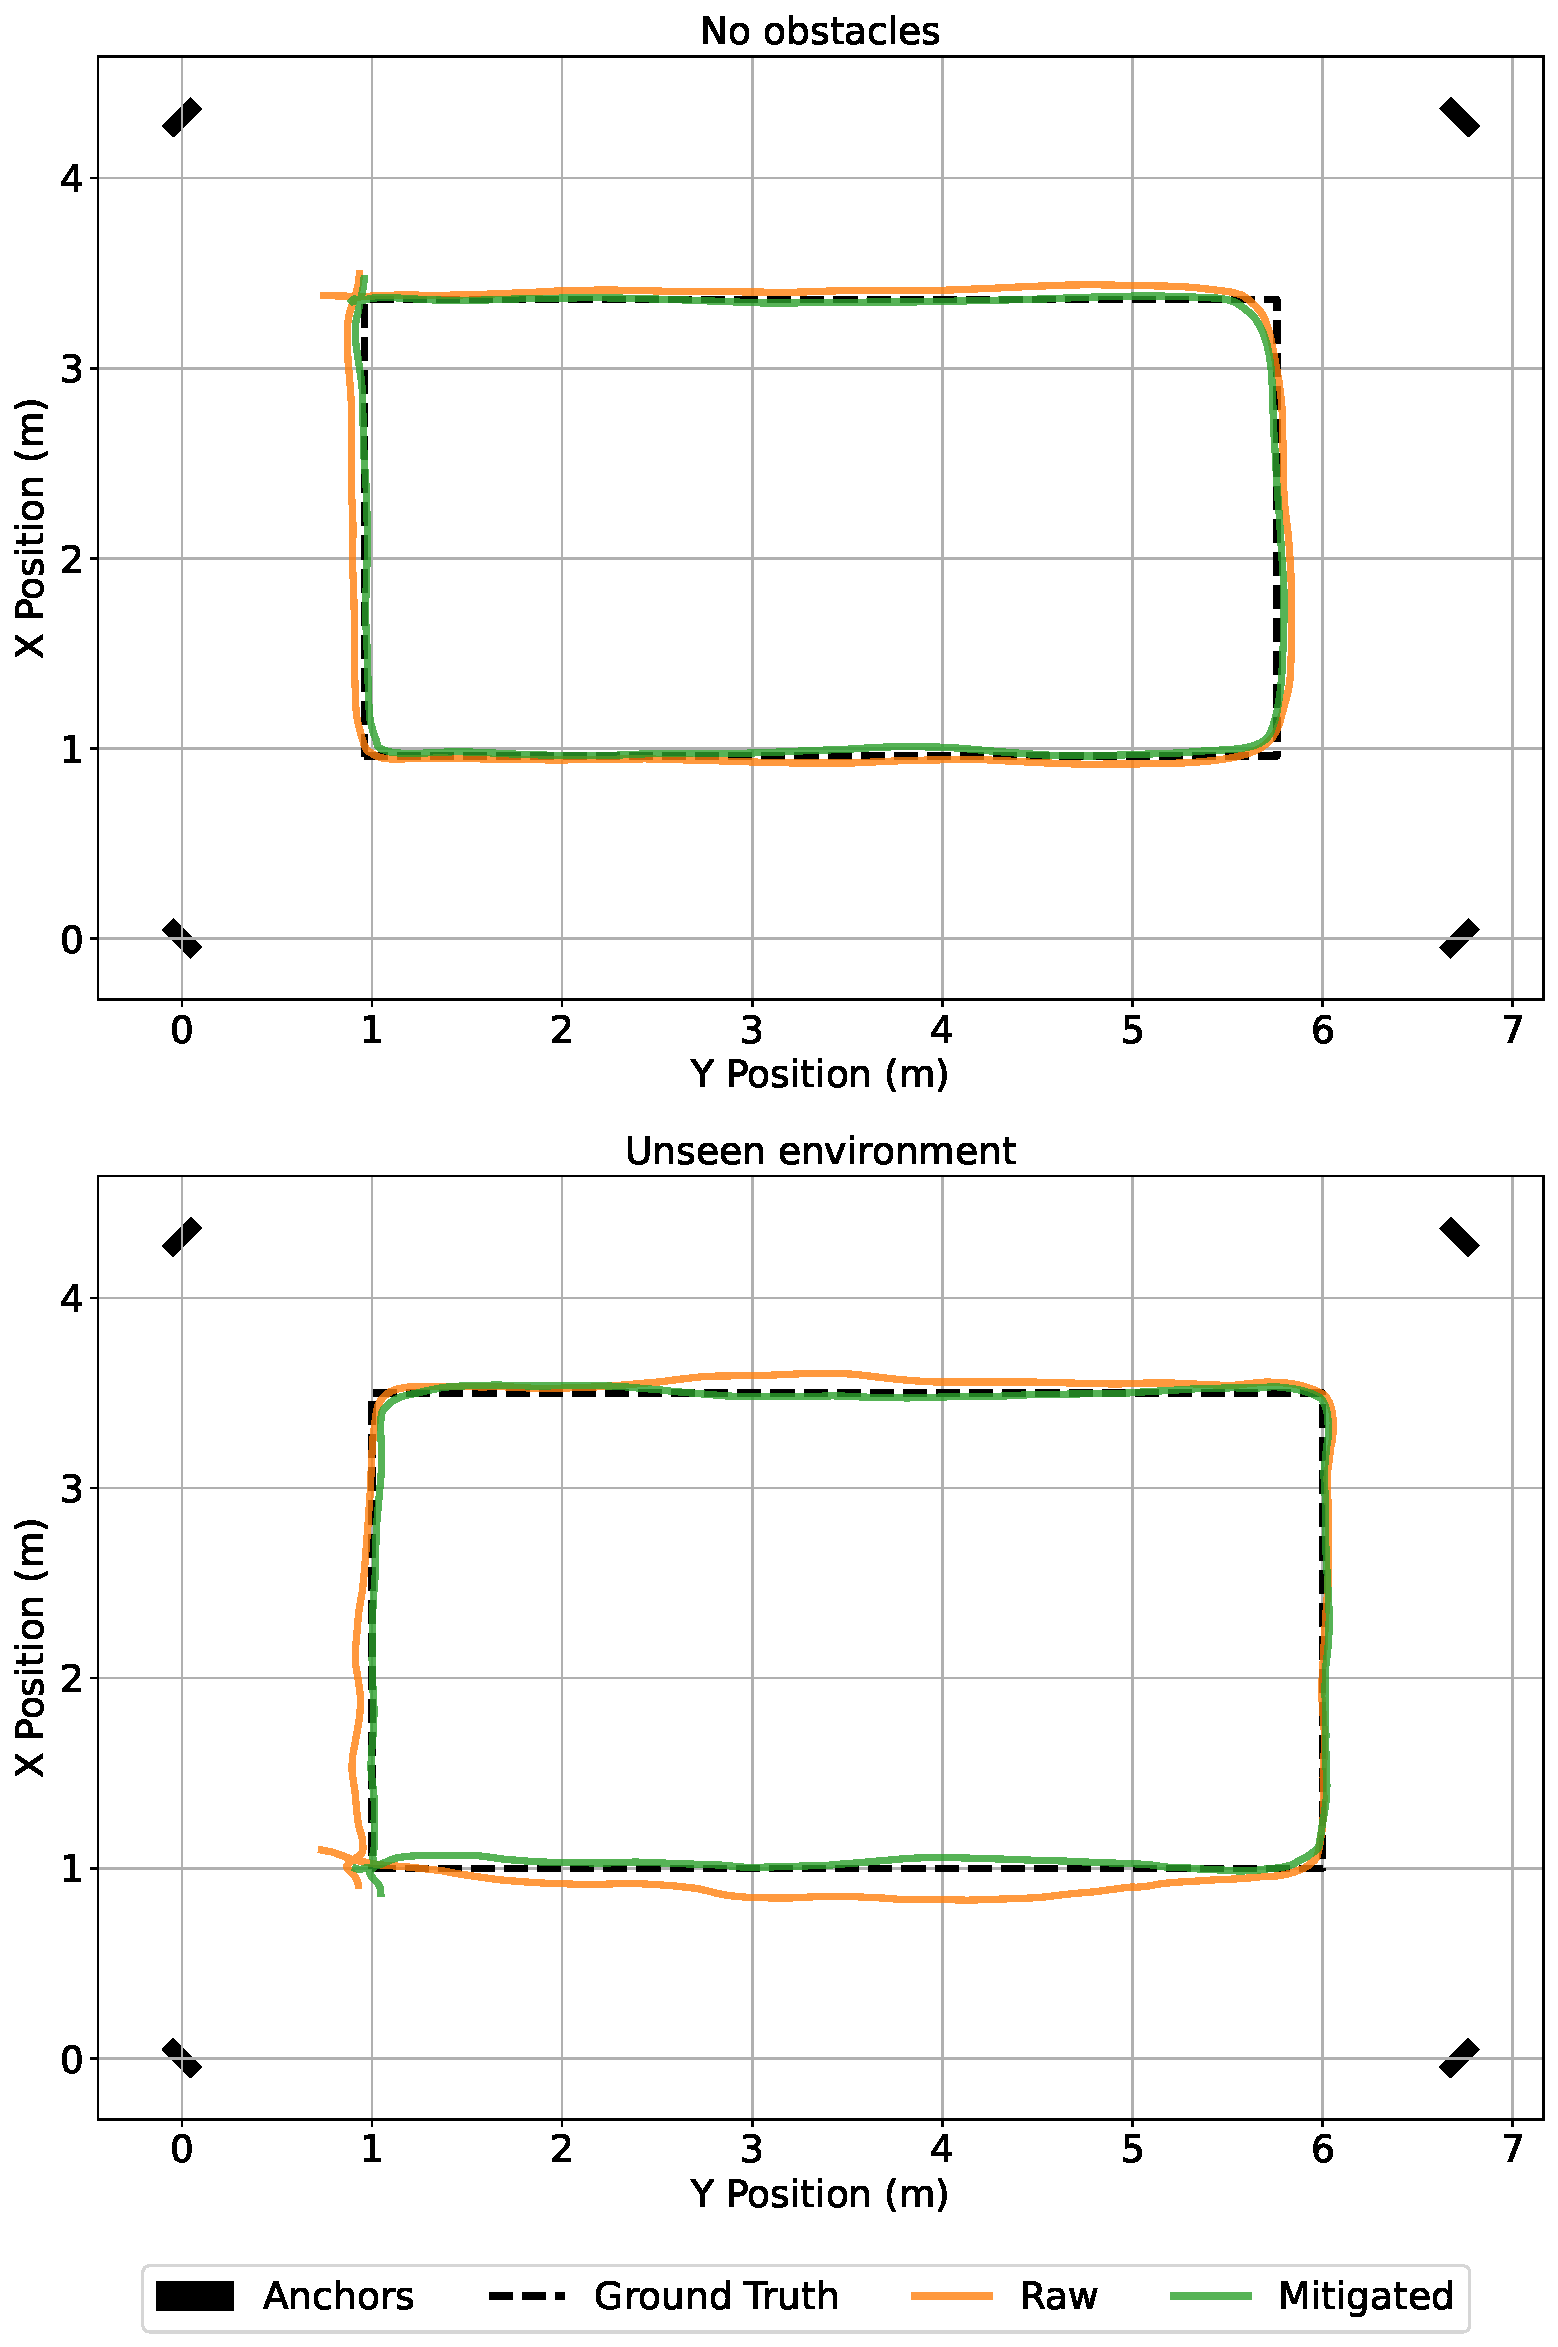
\includegraphics[width=0.85\textwidth]{Figures/experiments_and_results/rect_trajectory.pdf}
    \caption{Trajectory reconstruction results for the rectangular trajectory in both LoS (top) and unseen NLoS (bottom) scenarios.}
    \label{fig:trajectories_rectangle}
\end{figure}

% To illustrate typical performance visually, we present qualitative comparisons of raw versus mitigated estimates against ground truth, for the hourglass and rectangular trajectories in \autoref{fig:trajectories_hourglass}, and \autoref{fig:trajectories_rectangle}, respectively. 

To complement the quantitative results, we present visual examples of typical trajectory reconstruction performance for LoS and unseen NLoS conditions. \autoref{fig:trajectories_hourglass} and \autoref{fig:trajectories_rectangle} illustrate qualitative comparisons between raw and mitigated trajectories versus the ground truth, for the hourglass-shaped and rectangular paths, respectively.

In both cases, the mitigated trajectory has improved geometric alignment with the ground-truth. Even in the LoS case, where original trajectory does not exhibit significant deviations from the ground truth, the mitigated path more closely follows the true one, particularly around trajectory sides. In the unseen environment, where both the room geometry and structural properties, such as building materials and internal layout, differ from the training setup, uncorrected trajectories exhibit significant deviations along all path. The mitigated outputs, however, show considerably reduced overshoot, indicating that the proposed model effectively compensates for NLoS-induced bias despite the domain shift, demonstrating strong generalization.
 
\chapter{Conclusion}

\section{Discussion}
The primary aim of this work was to design, develop, and evaluate a robust UWB-based indoor positioning system capable of maintaining high accuracy in challenging environments. Therefore, to address the inherent limitations of UWB under obstructed conditions, we placed a particular emphasis on improving ranging accuracy through CIR-driven NLoS error mitigation. To this end, we developed a fully integrated, end-to-end localization framework comprising three principal contributions.

First, a custom UWB-based ranging system was designed and implemented on a novel hardware platform built around the SynchronicIT SFM10 module, which incorporates the NXP Trimension OL23D0 UWB chipset. Unlike prior studies relying predominantly on Qorvo (formerly Decawave) transceivers, this work pioneers the use of a new UWB platform in a research context. In controlled experiments under LoS conditions, the system demonstrated high baseline accuracy, with median ranging errors kept under \SI{\pm 5}{\centi\metre}. The proposed TDMA-based synchronization across multiple anchors achieved a per-anchor measurement rate of \SI{67}{\hertz}.

Second, a comprehensive dataset for NLoS error mitigation and channel-state identification was collected under controlled indoor conditions. Data were gathered in both clear-LoS and dynamically induced human-occlusion NLoS scenarios, with an optical tracking system automatically labeling each measurement. The resulting dataset, comprising nearly one million measurements with synchronized CIRs, was published to support further research~\cite{yaroshevych_2025_rangecir}.

Third, a learning-based error mitigation module was designed and developed to predict measurement errors based on CIR data. Extending the REMNet architecture, proposed by Simone Angarano et al.~\cite{Simone2021UWB}, the proposed A-REMNet model incorporates complex-valued CIR inputs and a temporal self-attention mechanism. The predicted range biases were used to correct raw estimates, which were subsequently fused via an EKF to produce position estimates. The performance of the proposed pipeline was assessed through experimental trajectory reconstruction trials, achieving up to \SI{70}{\percent} median reduction in mean absolute localization error under NLoS conditions -- from \SI{15.9}{\centi\metre} to \SI{4.4}{\centi\metre} in the training environment, and up to \SI{58}{\percent} improvement -- from \SI{9.3}{\centi\metre} to \SI{3.8}{\centi\metre} in the unseen one, compared with raw, non-mitigated trajectories. Notably, even in LoS conditions, the error was still reduced by up to \SI{39}{\percent}, despite relatively low initial values -- from 5.0 to 3.0 cm.

These results further support the conclusion, well-established in prior work, that CIR-based, learning-driven mitigation can effectively reduce UWB ranging errors in realistic NLoS conditions. Notably, compared to existing literature, which often assesses error mitigation methods in isolation, we present a more integrated and empirically validated approach, evaluating the proposed solution within a complete positioning system prototype, operating under dynamic conditions.

\section{Limitations and future work}

Despite the promising results, this study has several limitations. The evaluation was constrained to two indoor environments, with NLoS conditions induced only by human occlusion. While representative of many practical scenarios, these occlusions tend to introduce relatively low ranging bias. Consequently, further studies are required to assess performance in various environments and with stronger obstructions, such as structural barriers or vehicles, commonly found in industrial and automotive contexts. Moreover, only a single anchor deployment configuration was explored. Systematic studies of anchor density, geometry, and mounting strategies, such as ceiling-mounted configurations, which may exacerbate antenna polarization mismatches or increase GDOP, are needed to characterize their impact on positioning accuracy.

To improve generality, future work should also aim to expand the empirical dataset to include a wider spectrum of deployment scenarios, environments, and obstruction types. Additionally, examining the feasibility of on-device deployment of the proposed error mitigation model, particularly on embedded systems with constrained computational resources, would be beneficial for real-world scalability. The combination of CIR-driven models with unsupervised or semi-supervised learning frameworks also presents a compelling direction for reducing reliance on labeled datasets. Lastly, integrating this approach with other sensing modalities, such as inertial or visual systems, may further improve the robustness of the proposed system.

 

%----------------------------------------------------------------------------------------
%	BIBLIOGRAPHY
%----------------------------------------------------------------------------------------

\emergencystretch=1em
%% A.Y.: Allow Latex to apply emergency stretch to prevent overfull hboxes in bibliography

% \nocite{*}
\printbibliography[heading=bibintoc]

%----------------------------------------------------------------------------------------

\end{document}  
